\documentclass[12pt]{book}
\usepackage{mathptm,times,color}
\usepackage[pdftex]{graphicx}
\usepackage{hyperref}
\usepackage{multirow}
\usepackage{rotating}
\usepackage{longtable}
\usepackage{amsmath}
\usepackage{xfrac}

\usepackage{datetime}
\newdateformat{mydate}{\monthname[\THEMONTH] \THEYEAR}

\usepackage{listings}
\usepackage{textcomp}
\definecolor{lbcolor}{rgb}{0.96,0.96,0.96}
\lstset{
    %backgroundcolor=\color{lbcolor},
    tabsize=4,
    rulecolor=,
    language=Fortran,
        basicstyle=\footnotesize\ttfamily,
        upquote=true,
        aboveskip={\baselineskip},
        belowskip={\baselineskip},
        columns=fixed,
        extendedchars=true,
        breaklines=true,
        breakatwhitespace=true,
        frame=none,
        showtabs=false,
        showspaces=false,
        showstringspaces=false,
        identifierstyle=\ttfamily,
        keywordstyle=\color[rgb]{0,0,0},
        commentstyle=\color[rgb]{0,0,0},
        stringstyle=\color[rgb]{0,0,0},
}

\usepackage{wrapfig}

\renewcommand{\bibname}{References}

\setlength{\textwidth}{6.5in}
\setlength{\textheight}{9.0in}
\setlength{\topmargin}{0.in}
\setlength{\headheight}{0.in}
\setlength{\headsep}{0.in}
\setlength{\parindent}{0.25in}
\setlength{\oddsidemargin}{0.0in}
\setlength{\evensidemargin}{0.0in}

\begin{document}

\bibliographystyle{unsrt}

\newcommand{\asqh}{$A_T/A\sqrt{h}$}
\newcommand{\degc}{$^{\circ}$C }
\newcommand{\degf}{$^{\circ}$F }

\newcommand{\brackets}[1]{ { \left( {#1} \right) } }

\newcommand{\superscript}[1]{\ensuremath{^{\textnormal{#1}}}}
\newcommand{\subscript}[1]{\ensuremath{_{\textnormal{#1}}}}

\newcommand{\dx}{\delta x}
\newcommand{\dy}{\delta y}
\newcommand{\dz}{\delta z}
\newcommand{\dt}{\delta t}
\newcommand{\dQ}{\dot{Q}}
\newcommand{\dm}{\dot{m}}

\newcommand{\ha}{\frac{1}{2}}
\newcommand{\ft}{\frac{4}{3}}
\newcommand{\ot}{\frac{1}{3}}
\newcommand{\fofi}{\frac{4}{5}}
\newcommand{\of}{\frac{1}{4}}
\newcommand{\twth}{\frac{2}{3}}

\newcommand{\be}{\begin{equation}}
\newcommand{\ee}{\end{equation}}

\newcommand{\RE}{\hbox{Re}}
\newcommand{\PR}{\hbox{Pr}}
\newcommand{\NU}{\hbox{Nu}}

\newcommand{\COTWO}{{\tiny \hbox{CO}_2}}
\newcommand{\OTWO}{{\tiny \hbox{O}_2}}
\newcommand{\CO}{{\tiny \hbox{CO}}}
\newcommand{\HTWOO}{{\tiny \hbox{H}_2\hbox{O}}}
\newcommand{\NTWO}{{\tiny \hbox{N}_2}}
\newcommand{\F}{{\tiny \hbox{F}}}
\newcommand{\So}{{\tiny \hbox{S}}}
\newcommand{\M}{{\tiny \hbox{M}}}
\newcommand{\HCN}{{\tiny \hbox{HCN}}}
\newcommand{\HCl}{{\tiny \hbox{HCl}}}
\newcommand{\Hy}{{\tiny \hbox{H}}}
\newcommand{\C}{{\tiny \hbox{C}}}
\newcommand{\N}{{\tiny \hbox{N}}}
\newcommand{\Oh}{{\tiny \hbox{O}}}
\newcommand{\Cl}{{\tiny \hbox{Cl}}}
\newcommand{\rb}[1]{\raisebox{1.5ex}[0pt]{#1}}

\pagestyle{empty}

\begin{minipage}[t][9in][s]{6.5in}

\flushright{
    \fontsize{20}{24}\selectfont
    \bf{NIST Technical Note XXXX\\}
     }

\vspace{1in}

\flushright{
  \fontsize{28}{33.6}\selectfont
   \bf{CFAST -- Consolidated Model of Fire \\
   Growth and Smoke Transport \\
 \vspace{.25in}
   Volume 2: User's Guide \\}
   }
   
\vspace{.5in}

\flushright{
  \fontsize{14}{16.8}\selectfont
   Richard D. Peacock \\
   Paul A. Reneke \\
   Glenn P. Forney \\
}

\vspace{.5in}

\normalsize
\flushright{http://dx.doi.org/10.6028/NIST.TN.xxxxv2}

\vfill

\flushright{
\includegraphics[height=1.05in]{FIGURES/nistident}}

\end{minipage}

\newpage

\hspace{5in}

\newpage

\begin{minipage}[t][9in][s]{6.5in}

\flushright{
    \fontsize{20}{24}\selectfont
    \bf{NIST Technical Note XXXX\\
}
     }

\vspace{1.in}

\flushright{
  \fontsize{28}{33.6}\selectfont
   \bf{CFAST -- Consolidated Model of Fire \\
   Growth and Smoke Transport \\
\vspace{.25in}
   Volume 2: User's Guide \\}
   }

\vspace{.5in}

\normalsize
\flushright{
Richard D. Peacock \\
Paul A. Reneke \\
Glenn P. Forney \\
{\em Fire Research Division} \\
{\em Engineering Laboratory} 
 }
 
 \vspace{.5in}
 
\flushright{http://dx.doi.org/10.6028/NIST.SP.xxxxv2}

\vspace{.25in}

\flushright{\mydate\today\\
$SVN Repository$~$Revision: 831$}


\vfill

\flushright{
\includegraphics[width=1in]{FIGURES/doc} }

\small
\flushright{U.S. Department of Commerce \\
{\em Rebecca Blank, Acting Secretary} \\
\hspace{1in} \\
National Institute of Standards and Technology \\
{\em Patrick D. Gallagher, Under Secretary of Commerce for Standards and Technology and Director} }

\end{minipage}




\newpage

\frontmatter

\pagestyle{plain}
\setcounter{page}{3}

\chapter{Disclaimer}

The U. S. Department of Commerce makes no warranty, expressed or implied, to users of 
CFAST and associated computer programs, and accepts no responsibility for its use.  Users of 
CFAST assume sole responsibility under Federal law for determining the appropriateness of its 
use in any particular application; for any conclusions drawn from the results of its use; and for 
any actions taken or not taken as a result of analyses performed using these tools. 
CFAST is intended for use only by those competent in the field of fire safety and is intended 
only to supplement the informed judgment of a qualified user. The software package is a 
computer model which may or may not have predictive value when applied to a specific set of 
factual circumstances. Lack of accurate predictions by the model could lead to erroneous 
conclusions with regard to fire safety. All results should be evaluated by an informed user.

\chapter{Intent and Use}

The algorithms, procedures, and computer programs described in this report constitute a 
methodology for predicting some of the consequences resulting from a prescribed fire.  They 
have been compiled from the best knowledge and understanding currently available, but have 
important limitations that must be understood and considered by the user.  The program is 
intended for use by persons competent in the field of fire safety and with some familiarity with 
personal computers. It is intended as an aid in the fire safety decision-making process.

\chapter{Abstract}

CFAST is a two-zone fire model capable of predicting the environment in a multi-compartment structure subjected to a fire. It calculates the time evolving distribution of smoke and gaseous combustion products as well as the temperature throughout a building during a user-prescribed fire. This report describes the use of the model, including installing and running the software, the computer platforms upon which it is supported and examples to verify correct installation.

\chapter{Acknowledgments}

\label{acksection}

Continuing support for CFAST is via internal funding at NIST. In addition, support is provided by other agencies of the U.S. Federal Government, most notably the Nuclear Regulatory Commission Office of Research and the U.S. Department of Energy. The U.S. NRC Office of Research has funded key validation experiments, the preparation of the CFAST manuals, and the continuing development of sub-models that are of importance in the area of nuclear power plant safety. Special thanks to Mark Salley and David Stroup for their efforts and support. 

Support to refine the software development and quality assurance process for CFAST has been provided by the U.S. Department of Energy (DOE). The assistance of Subir Sen and Debra Sparkman in understanding DOE software quality assurance programs and the application of the process to CFAST is gratefully acknowledged. Thanks are also due to Allan Coutts, Washington Safety Management Solutions for his insight into the application of fire models to nuclear safety applications and detailed review of the CFAST document updates for DOE.

\tableofcontents

\listoffigures

\listoftables

\mainmatter


\chapter{Background}

CFAST is a two-zone fire model that predicts the thermal environment caused by a fire within a compartmented structure. Each compartment is divided into an upper and lower gas layer. The fire drives combustion products from the lower to the upper layer via the plume. The temperature within each layer is uniform, and its evolution in time is described by a set of ordinary differential equations derived from the fundamental laws of mass and energy conservation. The transport of smoke and heat from zone to zone is dictated by empirical correlations. Because the governing equations are relatively simple, CFAST simulations typically require a few tens of seconds of CPU time on typical personal computers.  The formulation of the equations, their solution, and discussion of validation and verification of the code are presented in companion documents \cite{CFAST_Tech_Guide_7, CFAST_Valid_Guide_7}.


\section{Input Data Required to Run the Model}

All of the data required to run the CFAST model reside in a single input file that the user generates. The file consists of the following information:
\begin{itemize}
\item compartment dimensions (height, width, length)
\item lining materials of the floor, walls, and ceiling of each compartment
\item material properties (e.g., thermal conductivity, specific heat, density, thickness, heat of combustion)
\item dimensions and positions of horizontal and vertical flow openings such as doors, windows, and vents
\item mechanical ventilation specifications
\item fire properties (e.g., heat release rate, lower oxygen limit, and species production rates as a function of time)
\item sprinkler and detector specifications
\item positions, sizes, and characteristics of targets
\end{itemize}
The input files are provided for the validation exercises described in the Validation Guide~\cite{CFAST_Valid_Guide_7}. A complete description of the theoretical and empirical formulation of the model can be found in the CFAST Technical Reference Guide~\cite{CFAST_Tech_Guide_7}.

A comprehensive assessment of the numerical parameters (such as default time step or solution convergence criteria) and physical parameters (such as empirical constants for convective heat transfer or plume entrainment) used in CFAST is not available in one document. Instead, specific parameters have been tested in various verification and validation studies performed at NIST and elsewhere. Numerical parameters are described in this Technical Reference Guide and are subject to the internal review process at NIST, but many physical parameters are extracted from the literature and do not undergo a formal review. The model user is expected to assess the appropriateness of default values provided by CFAST and make changes to the default values if need be.



\section{Model Results}

The output of CFAST are the sensible variables that are needed for assessing the environment in a building subjected to a fire. Once the simulation is complete, CFAST produces an output file containing all of the solution variables.  Typical outputs include (but are not limited to) the following:
\begin{itemize}
\item environmental conditions in the room (such as hot gas layer temperature; plume centerline temperature; oxygen and smoke concentration; and ceiling, wall, and floor temperatures)
\item heat transfer-related outputs to walls and targets (such as incident convective, radiated, and total heat fluxes)
\item fire intensity and flame height
\item flow velocities through vents and openings
\item detector and sprinkler activation times
\end{itemize}

Many of the outputs from the CFAST model are relatively insensitive to uncertainty in the inputs for a broad range of scenarios. However, the more precisely the scenario is defined, the more accurate the results will be. Not surprisingly, the heat release rate is the most important variable, because it provides the driving force for fire-driven flows. Other variables related to compartment geometry such as compartment height or vent sizes, while important for the model results, are typically more easily defined for specific design scenarios than fire related inputs.

\section{Model Version}

The first public release of CFAST was version 1.0 in June, 1990. This version was restructured from FAST~\cite{Models:FAST} to incorporate the ``lessons learned'' from the zone model CCFM developed by Cooper and Forney~\cite{Models:CCFM}. Version~2 was released as a component of Hazard~1.2 in 1994~\cite{Models:HAZARDI, Models:HAZARDI_12}. The first of the 3.x series was released in 1995 and included a vertical flame spread algorithm, ceiling jets and non-uniform heat loss to the ceiling, spot targets, and heating and burning of multiple objects (ignition by flux, temperature or time) in addition to multiple prescribed fires. As it evolved over the next five years, version~3 included smoke and heat detectors, suppression through heat release reduction, better characterization of flow through doors and windows, vertical heat conduction through ceiling/floor boundaries, and non-rectangular compartments. In 2000, version~4 was released and included horizontal heat conduction through walls, and horizontal smoke flow in corridors. Version~5 improved the combustion chemistry. Version 6, released in July, 2005, incorporates a more consistent implementation of vents, fire objects and event processing and includes a graphical user interface which substantially improves its usability.

The current version of CFAST, version 7, was released in 2015.


\chapter{Getting Started}

CFAST is documented by three publications, this user's guide, a technical reference guide~\cite{CFAST_Tech_Guide_7} and a model evaluation guide \cite{CFAST_Valid_Guide_7}. The technical reference guide describes the underlying physical principles, provides a comparison with other models, and includes an evaluation of the model following the guidelines of ASTM~E1355~\cite{ASTM:E1355}. The model evaluation guide documents verification and validation efforts for the model. This user's guide describes how to use the model.

\section{Installation}

CFAST was designed primarily for a personal computer running Microsoft Windows. However, the source code is written in Fortran and can be run as a stand alone command line application that reads input data from a text file. Details of how one runs CFAST without the Windows-based graphical user interface are found in Appendix~\ref{sec:CFAST_Keywords}. All of the files associated with CFAST can be obtained at:
\begin{lstlisting}
http://cfast.nist.gov
\end{lstlisting}
The CFAST distribution consists of a self-extracting set-up program for Windows-based personal computers. After downloading the set-up program, double-clicking on the file's icon walks the user through a series of steps for installation of the program.  The most important part of the installation is the creation of a folder (typically {\ct c:$\backslash$Program Files$\backslash$CFAST} by default) in which the CFAST executable files and supplemental data files are installed.  Sample input files are found in the {\ct Examples} folder. 

CFAST input files are best created and run using a Windows-based input editor called CEdit. Sample input files are provided with the program for new users who are encouraged to first run the sample calculations before attempting to create an input file. To run the model, browse to the location of the CFAST sample input file (default location is in a folder called {\ct Examples} in the installation folder, copy the file named {\ct standard.in} to a location of your choice and then double click on the copied file. This should open the file in the CFAST input editor, CEdit, as shown in Fig.~\ref{primary_screen}.
\begin{figure}[h!]
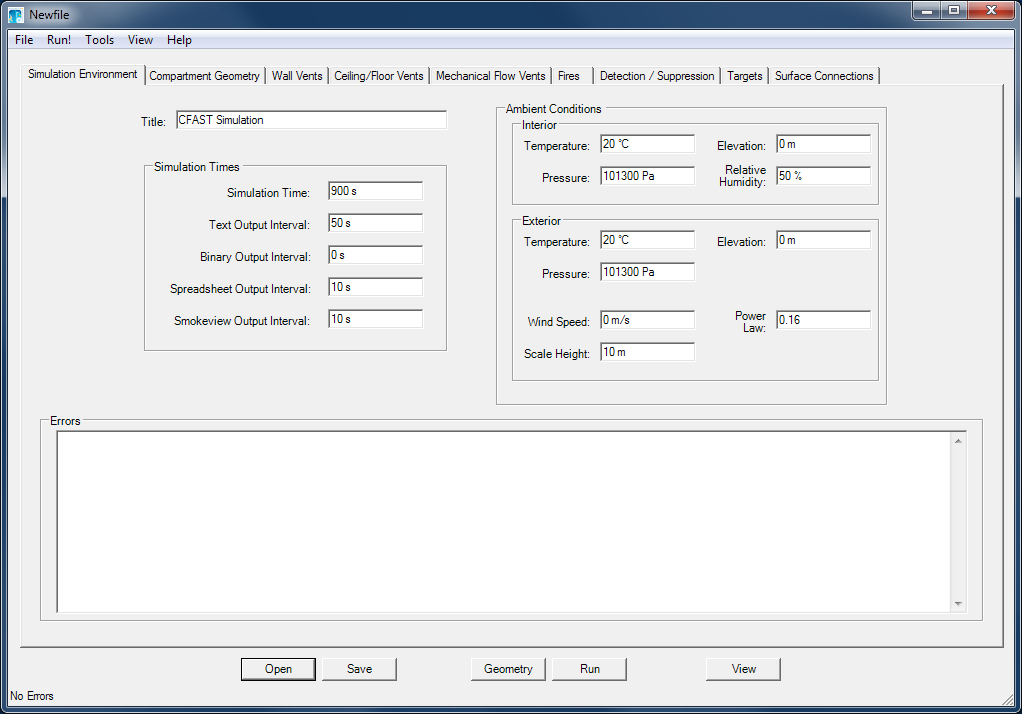
\includegraphics[width=6.5in]{FIGURES/Running_CFAST/Environment_Tab}
\caption[The primary CFAST input page]{The primary CFAST input page.}
\label{primary_screen}
\end{figure}
The simple test case can be run from the program menu by clicking on the ``Run'' icon. The case should finish in a few seconds. To verify that the installation has been done correctly, the output of the model should appear as shown in Fig.~\ref{Run_Model}.
\begin{figure}[h!]
\includegraphics[width=6.5in]{FIGURES/Getting_Started/Standard_Output}
\caption[The standard output screen]{The standard output screen.}
\label{Run_Model}
\end{figure}


\section{Basic Features}

The input parameters are organized via tabs near the top of the CEdit screen, as shown in Fig.~\ref{primary_screen}.
\begin{description}
\item[Simulation Environment] includes simulation time, specification of model outputs, and ambient conditions. Also included on the page are a constantly updated list of errors, warnings, and messages about the input file specification or model simulation.
\item[Compartments] defines the size, construction characteristics, and position of the compartments in a simulation.
\item[Wall Vents, Ceiling/Floor Vents, and Mechanical Ventilation] allows the user to connect compartments with doors and windows, ceiling and floor vents, or forced air ventilation systems.
\item[Fires] include user specification of the initial fire source and any additional burning objects in one or more of the compartments of the simulation.
\item[Detection / Suppression] defines any heat alarms and sprinklers in the compartments of the simulation.
\item[Targets] provide the ability calculate the temperature and net heat flux to objects placed and oriented arbitrarily in the structure.
\item[Surface Connections] allows for more detailed description of the connections between compartments in the simulation to better simulate the transfer of heat from compartment to compartment in the simulation.
\item[Visualizations] allows specification of one or more 2-D and 3-D visualizations to be added to the simulation for viewing with Smokeview. Note that these can require significant additional computational time than a basic CFAST simulation without visualizations.
\end{description}


\section{The Run! Menu}

The program includes a number of menu items for ancillary functions.  In addition to the normal file menu items to open and save input data files or to exit the program, a `Run!' menu is included to execute or view the current simulation. Menu items include the following:
\begin{description}
\item[Create Geometry File] for visualization with the program Smokeview.  The input data file is saved, if necessary, and CFAST is run with an option to only run through initialization. This is particularly useful to review placement of compartments, vents, and fires in a CFAST scenario. The resulting geometry can be viewed with the `Simulation Visualization, Smokeview' menu item, below.
\item[Model Simulation, CFAST] runs the case. The input file is saved, if necessary, and CFAST is run to completion.
\item[Simulation Visualization, Smokeview] runs the program Smokeview with the currently defined geometry.
\item[Output Options] include:
\begin{description}
\item[Detailed Output File] If checked, this menu item directs the CFAST model to produce a detailed text output file.  Details of the output files are included in Chapter~\ref{Output_Chapter}.
\item[Total Mass Output File] If checked, this menu item directs the CFAST model to replace the flow output with total mass flow through (mechanical) vents rather than the default flow rate values.
\item[Net Heat Flux]  If checked, this menu item directs the CFAST model to calculate heat flux to targets as a net heat flux to the target with the target at ambient temperature rather than at the calculated temperature.  This output is particularly useful to compare predictions to heat flux measurement using water cooled heat flux gauges.
\item[Show CFAST Window] If checked, this menu item allows the user to see the windows command prompt that is used to execute the CFAST model when the Model Simulation, CFAST menu item is used.  By default, this is not checked.  Normally, this can be left unchecked.  For troubleshooting, this can be selected to see additional details of the calculation as it progresses.
\item[CFAST Validation Output] If checked, this menu item directs the CFAST model to output an abbreviated heading for spreadsheet columns that are better for automated processing of the data. Heat fluxes are output as net heat flux to and ambient temperature target consistent with measurement with temperature-controlled heat fluxes gauges.
\end{description}
\end{description}


\section{The Edit Menu}


The `Edit' menu allows the user to view or change the material thermophysical properties and fire definitions used by the model and to select desired engineering units used in the input editor CEdit. Menu items include the following:
\begin{description}
\item[Edit Thermal Properties] allows you to define and manage property data used to describe compartment walls and targets.
\item[Edit Fires] allows you to define the heat release rate, pyrolysis rate, and species yields as a function of time for each fire.
\item[Select Engineering Units] allows you to select the units for input and output. By default, most outputs are in S.I. units, with temperature in Celsius.
\end{description}

\section{The View Menu}

The View menu allows you to view or print the input data file, output file (if the simulation has been run and a text output file generated) and the log file of the simulation. If one of the items does not exist on the user's hard disk, the selection is grayed out.

\section{The Help Menu}

The Help menu accesses this user's guide, the CFAST web site, or an about dialog box that displays the user license and version of the program.









\chapter{Running CFAST}

Running CFAST is relatively simple. All of the parameters that describe a given fire scenario are entered into a text file that is referred to as the "data" or "input" file. In this document, the data file is designated as filename.in, where "filename" stands for any character string that helps to identify the simulation. All of the output files associated with the calculation would typically have this common prefix. In addition to the input file, there are often several external files containing input parameters for the simulation. These files are referred to as "database" files, which contain parameters describing common materials and fuels.

The CFAST distribution includes a Windows-based input editor called CEdit that allows the user to enter details of a simulation in a standard Windows format, save the data file to disk, and run the simulation with CFAST from within the program.  Typically, all simulations would be developed and run from within CEdit.  For numerous, similar or lengthy simulations, the fire model CFAST can be run from a command prompt window.

It is suggested that a new user start with an existing data file, run it as is, and then make the appropriate changes to the input file for the desired scenario. By running a sample case, the user becomes familiar with the procedure and ensures that his/her computer is up to the task before embarking on learning how to create new input files.

\section{Creating a CFAST Input Data File}

All of the data to run the model is contained in an input data file. This file contains information about the building geometry (compartment sizes, materials of construction, and material properties), connections between compartments (horizontal flow openings such as doors, windows), vertical flow openings in floors and ceilings, and mechanical ventilation connections), fire properties (fire size and species production rates as a function of time), and specifications for detectors, sprinklers, and targets (position, size, heat transfer characteristics, and flow characteristics for sprinklers). Materials are defined by their thermal conductivity, specific heat, density, thickness, and burning behavior (heat release rate, ignition properties, and species yields).

The input data file provides the program with parameters to describe the scenario under consideration. The parameters are organized into groups of related variables. Each line of the input data file contains inputs related to a single group and begins with a keyword that identifies the input.  For example, compartment geometry is described by a set of lines (keyword COMPA) that define the width, depth, and height of each compartment.  A description of the input parameters can be found in Chapter 4.

Typically, the input data file will be created with the input editor, CEdit, included with the CFAST distribution. A shortcut to the input editor is placed on the start menu during installation.  To run, select Start, Program Files, and CFAST. Details of the program and its inputs are described in chapter 4.

\begin{figure}[h!]
\begin{center}
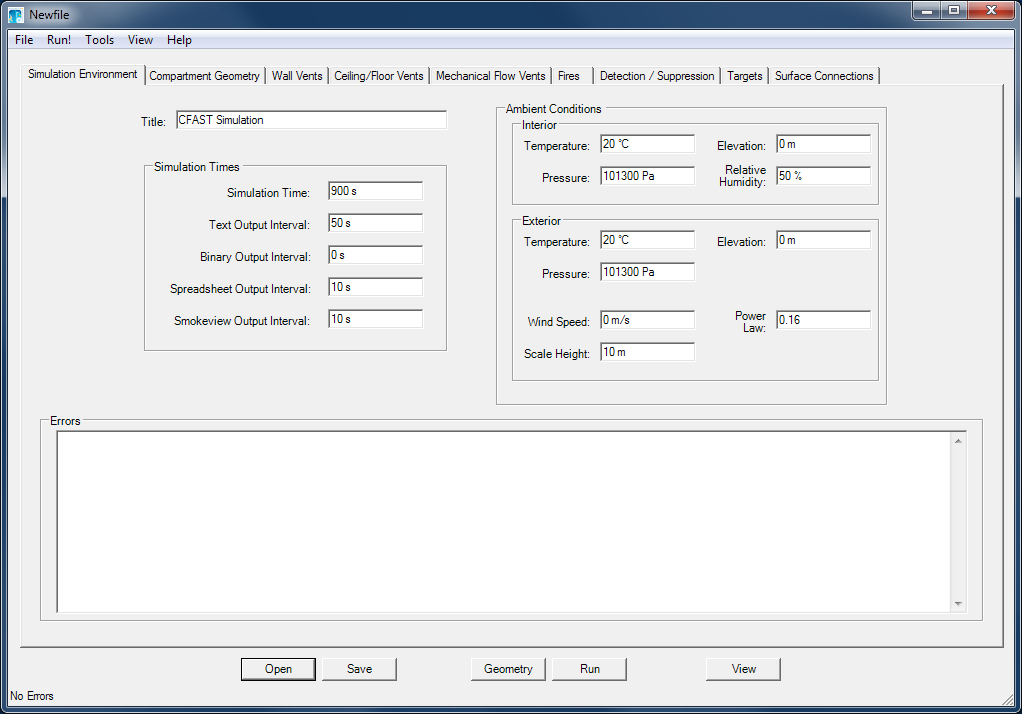
\includegraphics[width=6.5in]{FIGURES/Running_CFAST/Environment_Tab}
\end{center}
\end{figure}

\begin{wrapfigure}{l}{3in}
  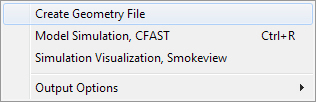
\includegraphics[width=3in]{FIGURES/Running_CFAST/Run_Menu}
\end{wrapfigure}

The program includes a number of menu items for ancillary functions.  In addition to the normal file menu items to open and save input data files or to exit the program, a 'Run!' menu is included to execute or view the current simulation. Menu items include the following:

\textbf{Create Geometry File:} used to create a geometry file for visualization with the program smokeview.  The input data file is saved, if necessary, and CFAST is run with an option to only run through initialization. This is particularly useful to review placement of compartments, vents, and fires in a CFAST scenario. The resulting geometry can be viewed with the 'Simulation Visualization, Smokeview' menu item, below.

\textbf{Model Simulation, CFAST:} runs the current input data file specification with the fire model CFAST.  The input data file is saved, if necessary, and CFAST is run to completion.  Additional details are described below in the section on starting a CFAST calculation. In order to visualize the results of the simulation with the program smokeview, the Smokeview Output Interval must be set to a non-zero value on the simulation Environment page.  This is described in more detail in chapter 4.

\textbf{Simulation Visualization, Smokeview:} runs the program smokeview with the previously defined smokeview geometry file. This allows the user to see the compartment geometry and connections or view the results of the simulation visually.  Additional details on the use of smokeview are included in the user's guide for Smokeview \cite{Smokeview_Users_Guide_6}.

\begin{figure}[h!]
\begin{center}
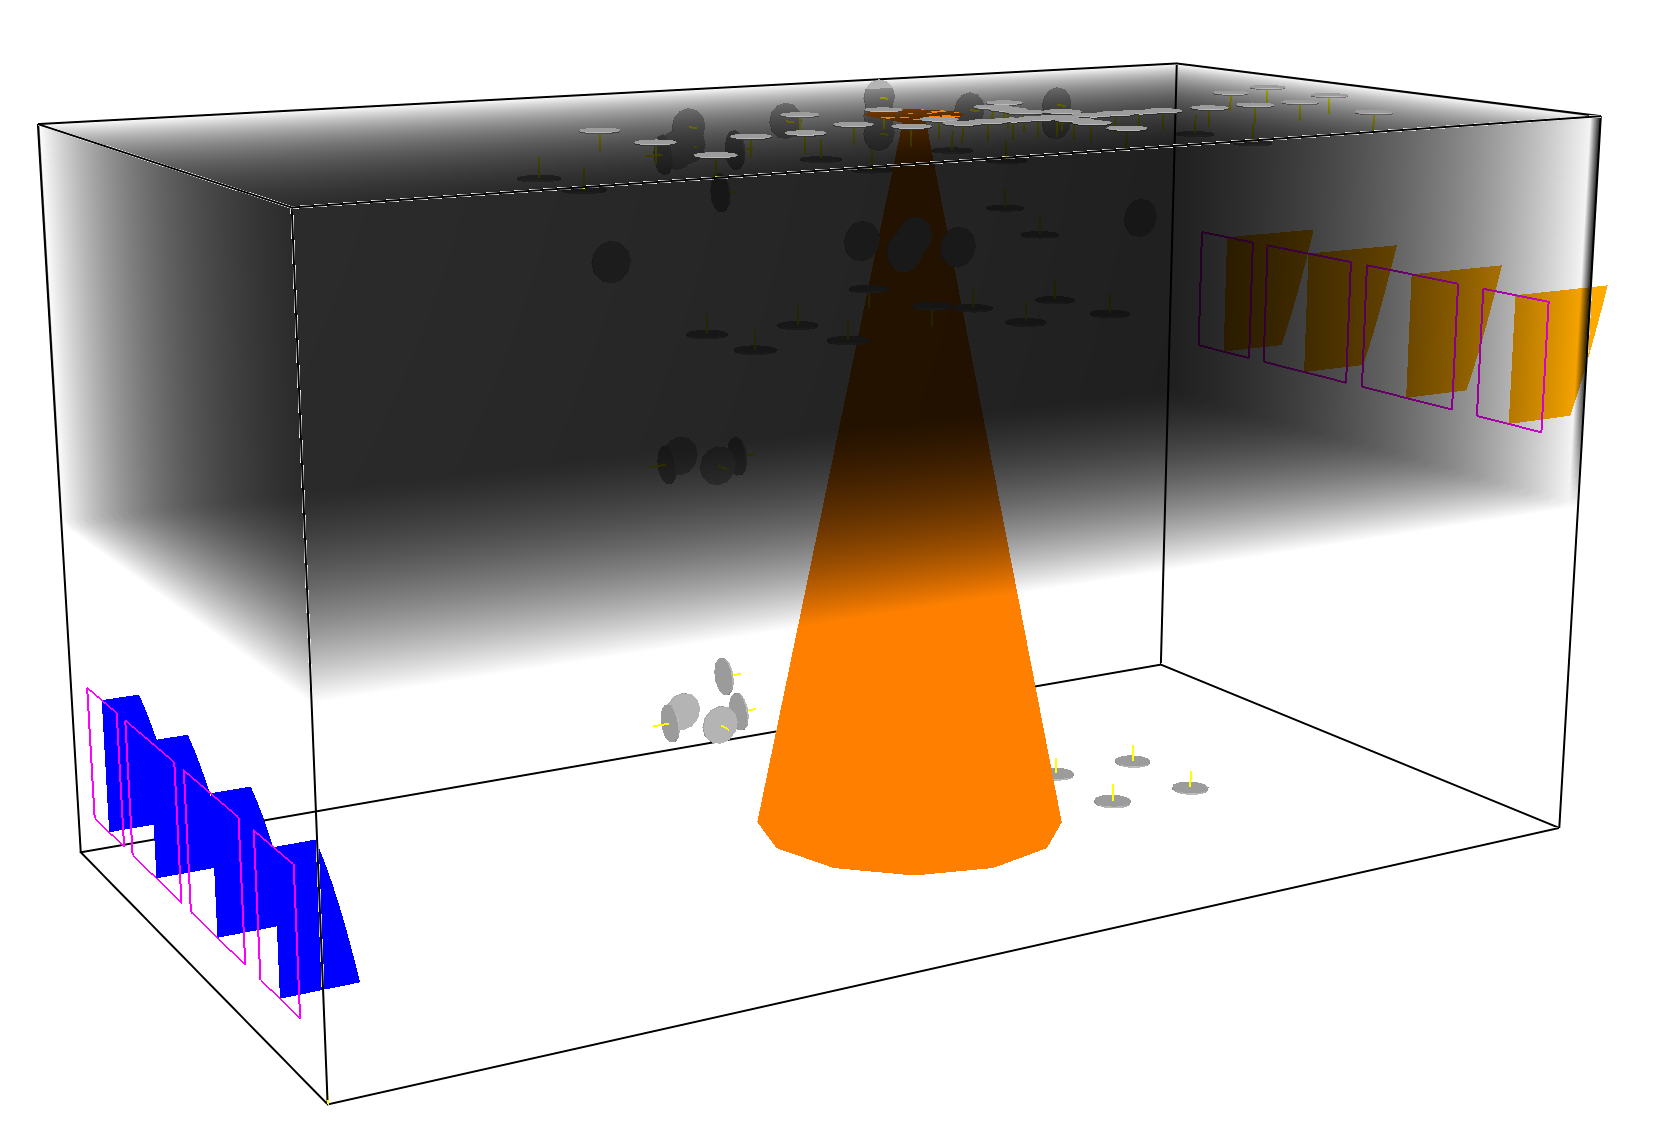
\includegraphics[width=6.5in]{FIGURES/Running_CFAST/Smokeview_Sample}
\end{center}
\end{figure}

\begin{wrapfigure}{l}{2.6in}
  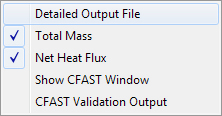
\includegraphics[width=2.6in]{FIGURES/Running_CFAST/Output_Options_Menu}
\end{wrapfigure}

Additional menu items can be selected to control details of the model simulation output using CFAST by selecting the Output Options submenu.

\textbf{Detailed Output File:} If checked, this menu item directs the CFAST model to produce a detailed text output file.  Details of the output are included in chapter 5.

\textbf{Total Mass Output File:} If checked, this menu item directs the CFAST model to replace the flow output with total mass flow through (mechanical) vents rather than the default flow rate values.

\textbf{Net Heat Flux:}  If checked, this menu item directs the CFAST model to calculate heat flux to targets as a net heat flux to the target with the target at ambient temperature rather than at the calculated temperature.  This output is particularly useful to compare predictions to heat flux measurement using water cooled heat flux gauges.

\textbf{Show CFAST Window:} If checked, this menu item allows the user to see the windows command prompt that is used to execute the CFAST model when the Model Simulation, CFAST menu item is used.  By default, this is not checked.  Normally, this can be left unchecked.  For troubleshooting, this can be selected to see additional details of the calculation as it progresses.

\textbf{CFAST Validation Output:} If checked, this menu item directs the CFAST model to output target fluxes at net heat flux and to output an abbreviated heading for spreadsheet columns that are better for automated processing of the data.


\begin{wrapfigure}{l}{2in}
  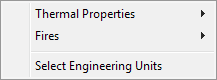
\includegraphics[width=2in]{FIGURES/Running_CFAST/Tools_Menu}
\end{wrapfigure}

The 'Edit' menu allows the user to view or change the material thermophysical properties and fire definitions used by the model and to select desired engineering units used in the input editor CEdit. Menu items include the following.

\textbf{Thermal Properties:} Heat transfer through compartment surfaces, to secondary fire objects, or other targets that may be specified depends on user-specified thermal properties for the materials.  These may be viewed, changed, or added to by the user as desired with the \textbf{Edit Thermal Properties} menu item. Materials properties include thermal conductivity, specific heat, density, thickness, and emissivity. Materials included in the database provided with the program are textbook values of common building and furnishing materials.

\begin{figure}[h!]
\begin{center}
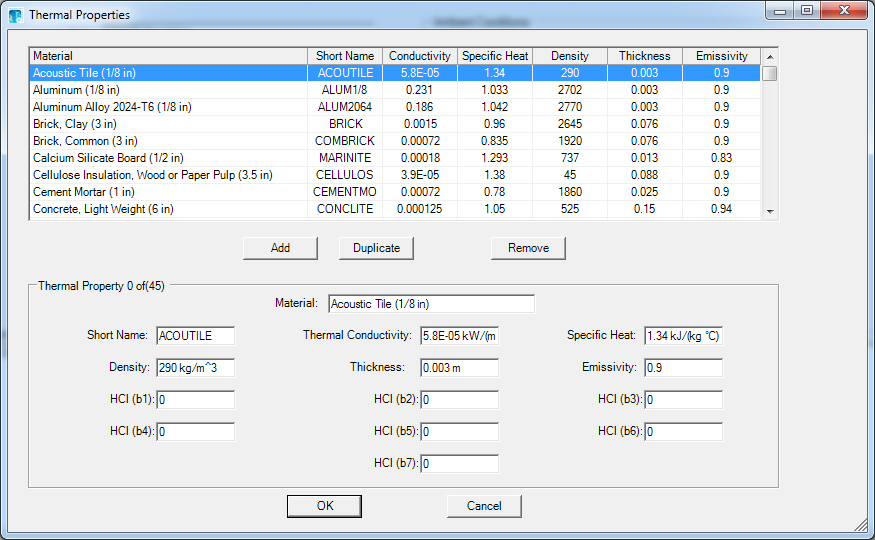
\includegraphics[width=6.5in]{FIGURES/Running_CFAST/Thermal_Properties_Edit}
Editing Thermal Properties in Cedit
\end{center}
\end{figure}

When CEdit is started, no thermal properties or fires are defined \label{Thermal_Properties_Menu}.  The \textbf{Insert Thermal Properties} menu item allows thermal properties used in a different simulation to be inserted into the data for the current simulation by choosing an existing CFAST input file and selecting one or more of the thermal properties to be included in the current simulation.

\begin{figure}[h!]
\begin{center}
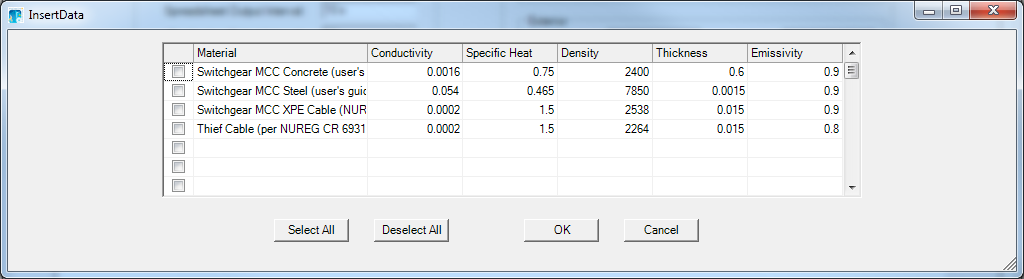
\includegraphics[width=6.5in]{FIGURES/Running_CFAST/Thermal_Properties_Insert}
Inserting Thermal Properties in Cedit
\end{center}
\end{figure}

\newpage

\textbf{Fires:} Fires in CFAST are defined with one or more selected fire objects that define the heat release rate, pyrolysis rate, and species yields as a function of time for each fire.  These may include the default set of fire objects included with the software or additional or modified objects created by the model user. They may be viewed or changed by the user as desired with the \textbf{Edit Fires} menu item \label{Fires_Menu}.

\begin{figure}[h!]
\begin{center}
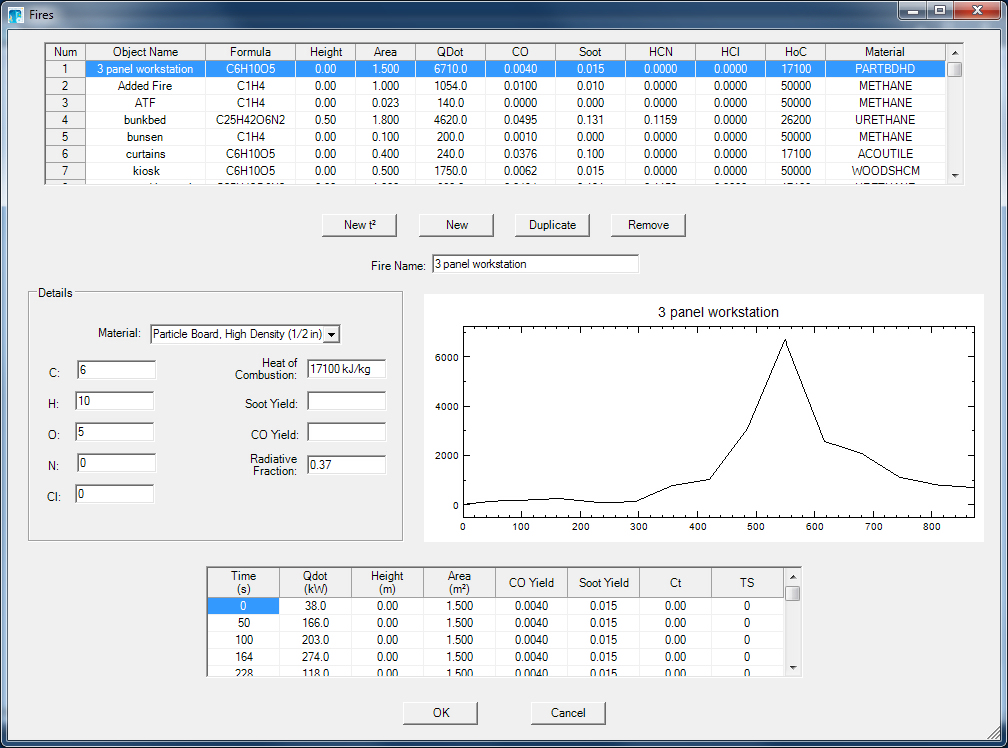
\includegraphics[width=6.5in]{FIGURES/Running_CFAST/Fire_Objects_Edit}
Editing Fires in CFAST
\end{center}
\end{figure}
\newpage

When CEdit is started, no thermal properties or fires are defined.  The \textbf{Insert Fires} menu item allows fire definitions used in a different simulation to be inserted into the data for the current simulation by choosing an existing CFAST input file and selecting one or more of the fires to be included in the current simulation.

\begin{figure}[h!]
\begin{center}
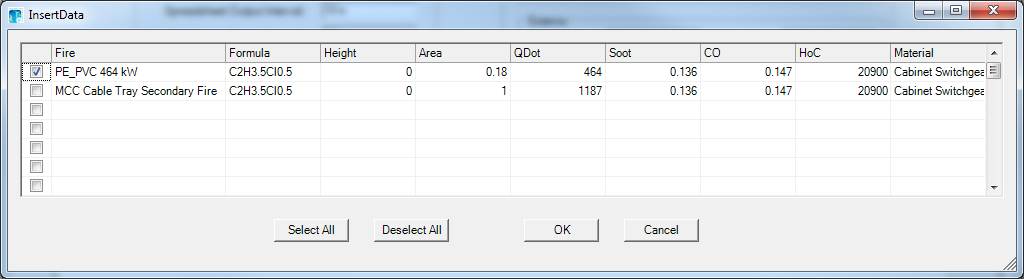
\includegraphics[width=6.5in]{FIGURES/Running_CFAST/Fire_Objects_Insert}
Inserting Fires in Cedit
\end{center}
\end{figure}

Details of fire objects and parameters included on the fire objects window are included in the section on object fires in the next chapter.

\textbf{Select Engineering Units:} The CFAST model uses input values and provides output in S.I. units. Within the input editor, CEdit, the user may select engineering units of choice for input and output.  These values are saved in the windows registry and may be changed at any time. By default, most outputs are in S.I. units, with temperature in Celsius.

\begin{figure}[h!]
\begin{center}
  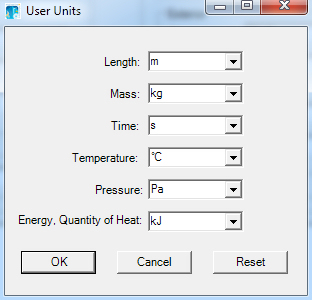
\includegraphics[width=3in]{FIGURES/Running_CFAST/Select_Engineering_Units}
\end{center}
\end{figure}

\clearpage

\begin{wrapfigure}{r}{1.95in}
  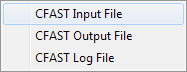
\includegraphics[width=1.95in]{FIGURES/Running_CFAST/View_Menu}
\end{wrapfigure}

The View menu allows the user to view and / or print the input data file, output file (if the simulation has been run and a text output file generated) and the log file of the simulation. If one of the items does not exist on the user's hard disk, the selection is grayed out. \\~ \\

\begin{wrapfigure}{r}{1.88in}
  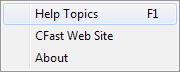
\includegraphics[width=1.88in]{FIGURES/Running_CFAST/Help_Menu}
\end{wrapfigure}
 The Help menu accesses this user's guide, the CFAST web site, or an about dialog box that displays the user license and version of the program. \\~ \\

\section{File Naming and Location}

By default, the CFAST installation places all program files in the directory 'c:$\backslash$Program Files$\backslash$CFAST6' (or directory 'c:$\backslash$Program Files (x86)$\backslash$CFAST6'  on Windows 7 machines) and sample input data files in the 'Examples' folder included in the installation directory, While these locations can be changed during installation, the documentation in this user's guide assumes these locations.

In addition, there are several files that CFAST uses to communicate with its environment.  They include 1) an input data file, required for every simulation, 2) a series of spreadsheet files of important output variables, and binary data files containing calculated values for visualization the simulation.  Documentation of the input data file is included as chapter 4 of this user's guide.

In CFAST, simulations are arranged as projects with all the files associated with a single simulation sharing a common base file name.  For a simulation with a base file name of 'project', the built-in naming conventions would identify the files of the simulation as follows:

\begin{itemize}
\item input: project.in
\item text output file: project.out
\item spreadsheet output files: (Normal output) project\_n.csv, (Species output) project\_s.csv, (Flow output) project\_f.csv, (Wall surface temperatures, targets and sprinklers) project\_w.csv
\item smokeview geometry file: project.smv
\item smokeview plot file: project.zone
\item smokeview slice file(s): project\_\#\#\#\#.sf (where \#\#\#\# is a four digit number automatically assigned by the software)
\item smokeview iso-surface file(s): project\_\#\#\#\#.iso (where \#\#\#\# is a four digit number automatically assigned by the software).
\end{itemize}

There may be additional files associated with a specific simulation.  Any fires defined for the simulation (fire object files are defined with a .o extension) and customized thermal properties may be included in a revised thermal.csv file.  These must be in the same directory as the input file for the model to run.

\section{Starting a CFAST Calculation}

\subsection{Running CFAST from CEdit}

Typically, model simulations are run directly from the input editor, CEdit.  To run the model, either open an existing input data file from the program menus with 'File', 'Open,' or create a new input data file within CEdit.  The model is run by selecting 'Run!' and then 'Model Simulation, CFAST.'

This opens a window that shows the progress of the simulation, with information on the environment in each compartment of the simulation.

\begin{figure}[h!]
\begin{center}
\includegraphics[width=6.5in]{FIGURES/Running_CFAST/Standard_Output}
\end{center}
\end{figure}

Several buttons are also available as follows:

\begin{wrapfigure}{l}{0pt}
  
\includegraphics[width=0.79in]{FIGURES/Running_CFAST/Close_Button}
\end{wrapfigure}

The close button is disabled while the model is running.  Once the simulation is complete (stopped by the user with the stop button), the close button closes the window and returns to the main input editor. \\

\begin{wrapfigure}{l}{0pt}
  
\includegraphics[width=0.79in]{FIGURES/Running_CFAST/Stop_Button}
\end{wrapfigure}

 The stop button halts execution of the simulation, but leaves the simulation window on the screen.  The stop button is available only when the simulation is in progress. \\

Normally, model outputs are displayed and updated only at any of the time intervals specified on the environment page. For complex calculations, there may be a significant time period between display updates. The update button allows the user to see the current state of the calculation at any time. The update button is only available when the simulation is in progress.

\subsection{Running CFAST from a Command Prompt}

The model CFAST can also be run from a Windows command prompt.  CFAST can be run from any folder, and refer to a data file in any other folder. The fires and thermophysical properties have to be in either the data folder, or the executable folder. The data folder is checked first and then the executable folder.

\begin{lstlisting}
[drive1:\][folder1\]cfast [drive2:\][folder2\]project
\end{lstlisting}

The project name will have extensions appended as needed (see below). For example, to run a test case when the CFAST executable is located in c:$\backslash$nist$\backslash$cfast6 and the input data file is located in c:$\backslash$data, the following command could be used:

\begin{lstlisting}
c:\nist\cfast6\cfast c:\data\testfire0   <<< note there is no extension.
\end{lstlisting}

If the command is entered as $\backslash$bin$\backslash$cfast $\backslash$bin$\backslash$data$\backslash$testfire0.in, then CFAST will try to open testfire0.in.in

The database files for thermal properties and fire objects may be located either in the folder with the input data file or in the folder with the CFAST executable. The model checks first in the data file folder and then in the CFAST executable folder.  If the files do not exist in either location, the simulation is not run. By default, names for these files are thermal.csv for the thermal properties file and *.o for the fire object files.

Command line options

\begin{itemize}
\item k - no keyboard access
\item i - initialization only
\item h - output header
\item c - compact output
\item f - full output (c and f are exclusive). Note the interaction of the f and c option. The default for the console output is /c. The default for the file output is /f. This default action can be overwritten by explicitly including the /f or /c option. Output goes to the screen if the print interval (second entry on the TIMES line) is positive and to the output file if the interval is negative.
\item t - replace the flow output with total flow through (mechanical) vents.
\item n - net heat flux option
\item v - validation output (outputs a modified set of spreadsheet files with different column headers designed to facilitate automated analysis of the output)
\end{itemize}

\chapter{Simulation Environment}

The Environment page defines the initial conditions and simulation time for the CFAST input file.

\begin{figure}[ht]
\centering
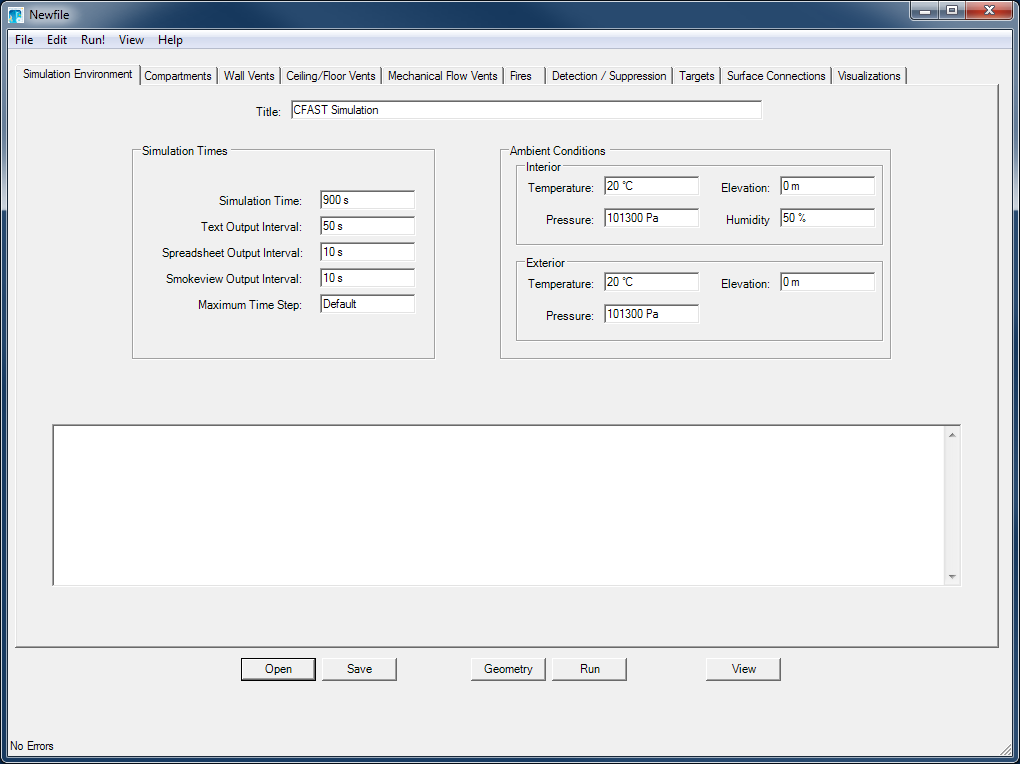
\includegraphics[width=6.5in]{FIGURES/Input_File/Environment_Tab}
\end{figure}

\section{Title}

The first thing to do when setting up an input file is to give the simulation a title. The title is optional and may consist of letters, numbers, and/or symbols and may be up to 50 characters. All output files will be tagged with this character string.


\section{Simulation Times}

\begin{description}
\item[Simulation Time] (default units: s, default value, 900 s): The length of time over which the simulation takes place. The maximum value for this input is 86400 s (1 day).

\item[Text Output Interval] (default units: s, default value, 50 s): The time interval between each printing of the output data.  If omitted or less than or equal to zero, no output values will appear.

\item[Spreadsheet Output Interval] (default units: s, default value, 10 s): CFAST can output the results of the simulation in a comma-delimited spreadsheet file. This parameter defines the time interval between these outputs. A value greater than zero must be used if the spreadsheet file is desired.

\item[Smokeview Output Interval] (default units: s, default value: 10 s): CFAST can output a subset of the results in a format compatible with the visualization program Smokeview. This input defines the time interval between outputs of the model results in a Smokeview-compatible format.  A value greater than zero must be used if the spreadsheet output is desired.

\item[Maximum Time Step] (default units: s, default value: 2 s): CFAST will automatically adjust the time interval for the solution of the differential equation set up or down so that the simulation is as efficient as possible within the pre-defined error tolerances. This parameter places a maximum value for the equation solver and can normally be left at the default value. In cases (which are hopefully rare) where the model fails to converge on a solution, this value can be reduced which often will allow the simulation to successfully complete.
\end{description}

\section{Ambient Conditions}

Ambient conditions define the environment at which the scenario begins. Initial pressures in a structure are calculated simply as a lapse rate (related to the height above sea level) based on the NOAA/NASA tables \cite{GPO:Atmosphere}. It is convenient to choose the base of a structure to be at zero height and then reference the height of the structure with respect to that height.  The temperature and pressure must then be measured at that position.  Another possible choice would be the pressure and temperature at sea level, with the structure elevations then given with respect to mean sea level.  This is also acceptable, but somewhat more tedious in specifying the construction of a structure.  Either of these choices works though, so long as they are consistent. Usually, the station elevation is set to zero and the pressure to ambient. The effect of changing these values is minor. Note that the equations implemented in the model are not designed to handle negative elevations and altitudes.

\begin{description}
\item[Temperature] (default units: \degc, default value: 20 \degc): Initial ambient temperature inside or outside the structure at the station elevation.

\item[Pressure] (default units: Pa, default value: 101300 Pa): Initial values for ambient atmospheric pressure inside and outside the structure at the station elevation. The default value is standard atmospheric pressure at sea level.

\item[Elevation] (defaults units: m, default value: 0 m): The height where the ambient pressure and temperature are specified.  This is the reference height for calculating the density of the atmosphere as well as the temperature and pressure inside and outside of the structure as a function of height.

\item[Humidity] (default units \% RH, default value: 50 \%): The initial relative humidity in the system, only specified for the interior.  This is converted to kilograms of water per cubic meter as an initial condition for both the interior and exterior of the structure.
\end{description}






\chapter{Compartments}

\begin{figure}[h!]
\begin{center}
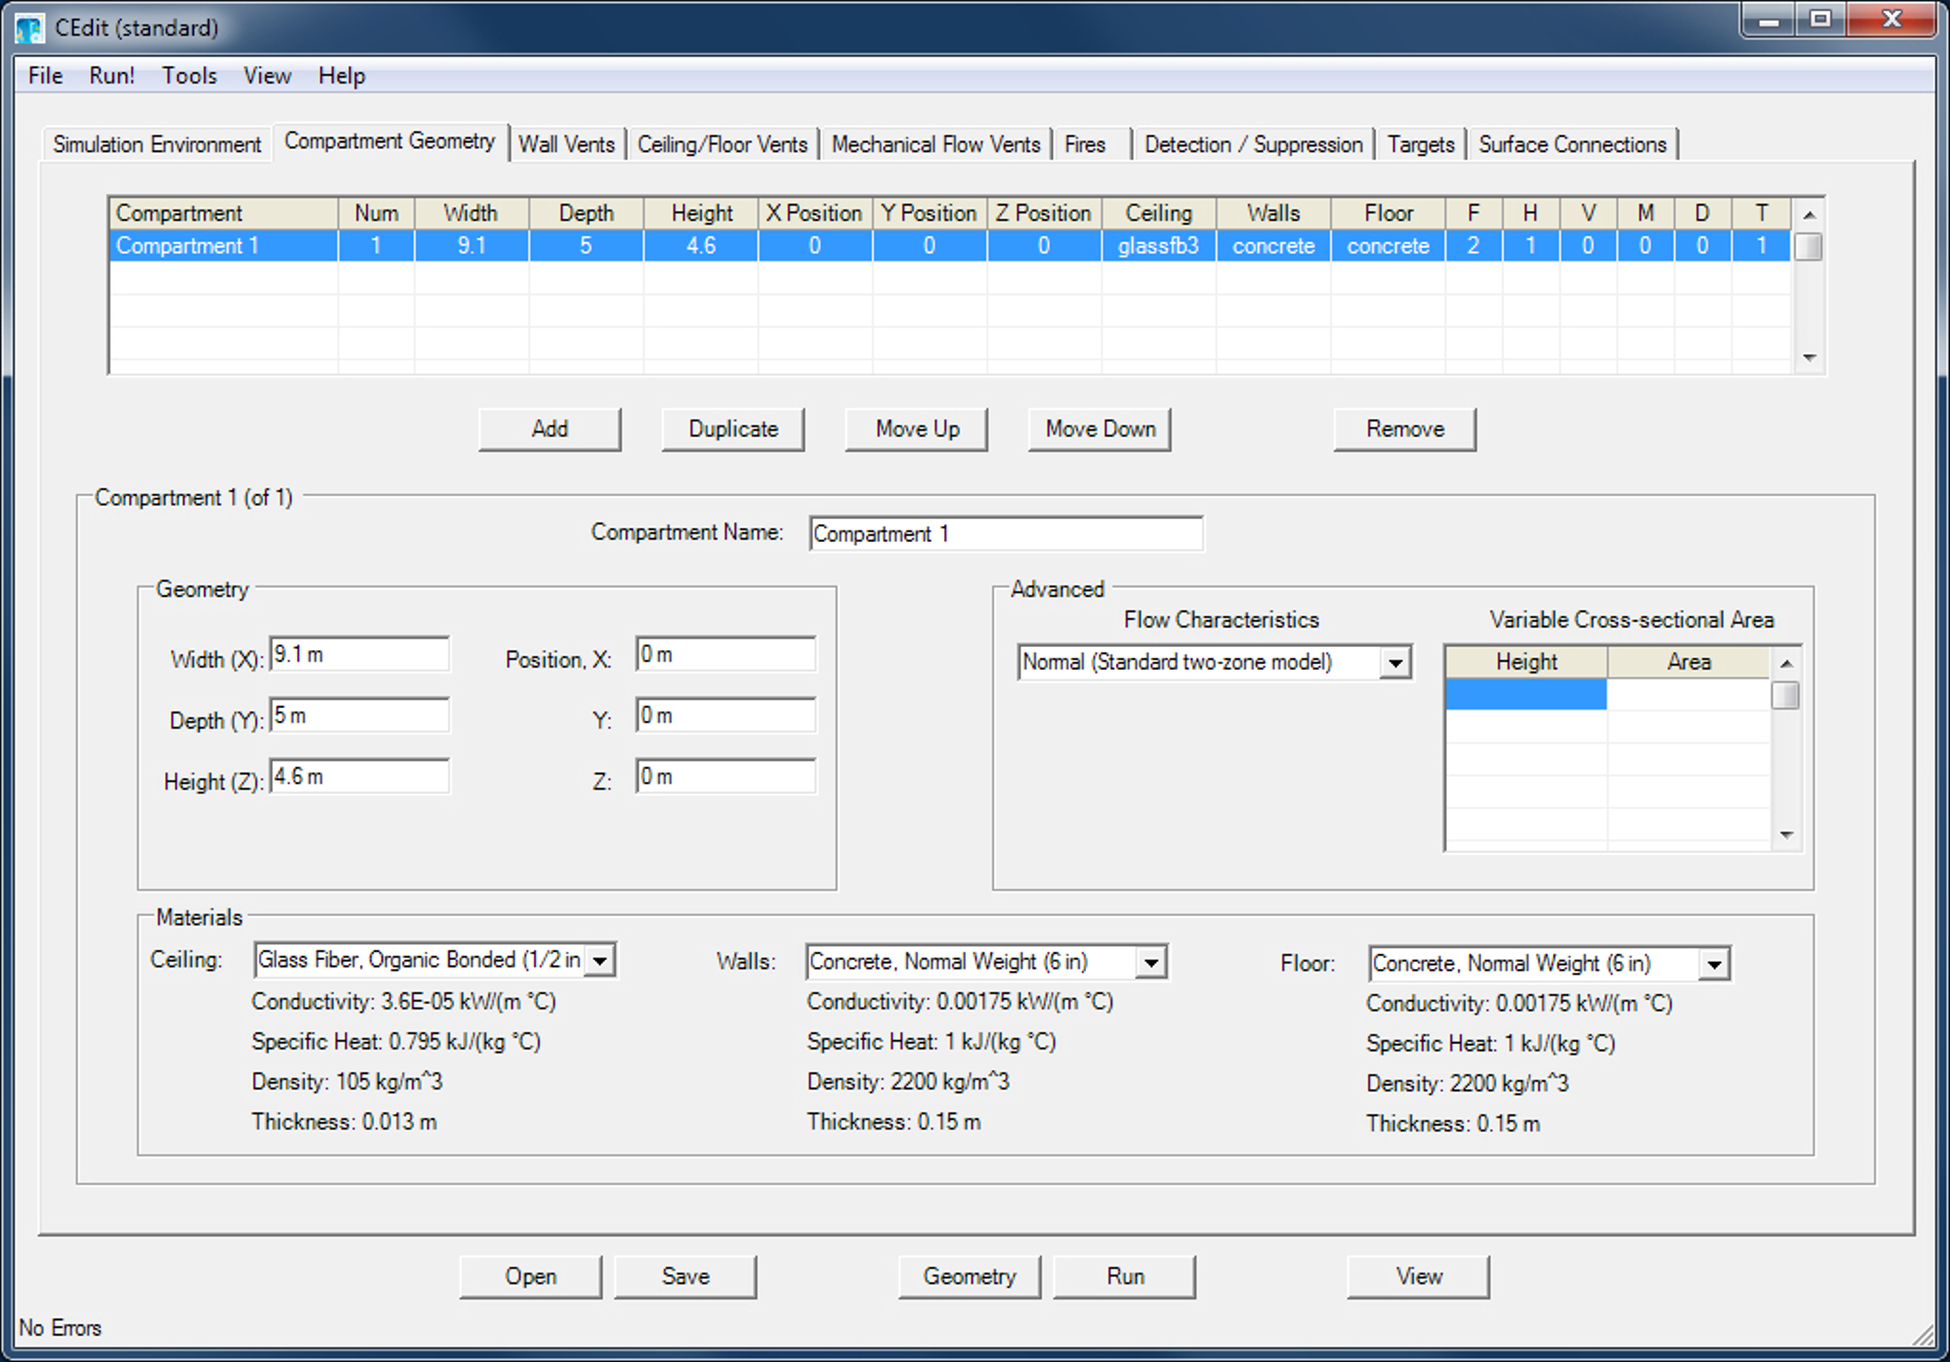
\includegraphics[width=6.5in]{FIGURES/Input_File/Compartment_Geometry_Tab}
\end{center}
\end{figure}

The Compartments page defines the size, position, materials of construction, and flow characteristics for the compartments in the simulation. Initially, only the simulation environment page and the 'Add' button on the compartment geometry page is enabled; all other pages are not available to the user for detailed inputs until a compartment has been added to the simulation.

In order to model a fire scenario, the size and position of each compartment in the structure must be specified. For a compartment, the width, depth, compartment height and height of the floor of the compartment provide this specification. The maximum number of compartments for version 6 is thirty. The usual assumption is that compartments are rectangular parallelepipeds. However, the CFAST model can accommodate odd shapes as equivalent floor area parallelepipeds or with a cross-sectional area that varies with height.

\begin{figure}[h!]
\begin{tabular*}{\textwidth}{c@{\extracolsep{\fill}}c}
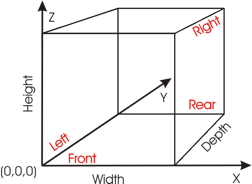
\includegraphics[width=2.5in]{FIGURES/Input_File/CFAST_Coordinates} &
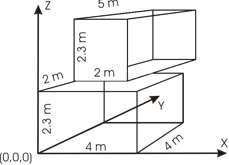
\includegraphics[width=2.6in]{FIGURES/Input_File/CFAST_Absolute_Positioning} \\
Compartment Size & Compartment Position
\end{tabular*}
\end{figure}

At least one compartment must be specified in the input file.  There are no defaults for compartment size. There are defaults for absolute positioning (0,0,0). The fully mixed (single zone) and corridor models are turned off by default.

\label{Compartment_Geometry}Compartments in CFAST are most typically defined by a width, depth, and height.  If desired, compartments can be prescribed by the cross-sectional area of the compartment as a function of height from floor to ceiling for other shapes. The absolute position of the compartment with respect to a single structure reference point can be defined to ease visualization or to allow exact placement of vents and surfaces relative to other compartments in a detailed calculation. This specification is important for positioning the compartments for visualization in Smokeview.

\begin{description}
\item[Compartment Name:] Compartments are identified by a unique alphanumeric name.  This may be a simple as a single character or number, or a description of the compartment.
\end{description}

\section{Geometry}

\label{Compartment_Inputs}
\begin{description}
\item[Width] specifies the width of the compartment as measured on the X axis from the origin (0,0,0) of the compartment.

\item[Depth] specifies the depth of the compartment as measured on the Y axis from the origin (0,0,0) of the compartment.

\item[Height] specifies the height of the compartment as measured on the Z axis from the origin (0,0,0) of the compartment.

\item[Absolute Width Position (Position X)] specifies the absolute x coordinate of the lower, left, front corner of the room.

\item[Absolute Depth Position (Position Y)] specifies the absolute y coordinate of the lower, left, front corner of the room.

\item[Absolute Floor Height (Position Z)] specifies the height of the floor of each compartment with respect to station elevation specified by the internal ambient conditions reference height parameter.  The reference point must be the same for all elevations in the input data.  For example, the two rooms in the sample to the right would be located at (0,0,0) and (0,2,2.3).
\end{description}

\section{Materials}

To calculate heat loss through the ceiling, walls, and floor of a compartment, the properties of the bounding surfaces must be known. This includes the thermophysical properties of the surfaces and the arrangement of adjacent compartments if inter-compartment heat transfer is to be calculated.

The bounding surfaces are the ceilings, walls and floors that define a compartment. These are referred to as thermophysical boundaries, since each participates in conduction and radiation as well as defining the compartments, unless these phenomena are explicitly turned off.

The thermophysical properties of the surfaces which define compartments are described by specifying the thermal conductivity, specific heat, emissivity, density, and thickness of the enclosing surfaces for each material and then assigning the material to the ceiling, walls, and floor of a compartment.  Thermal properties for materials are read from the CFAST input file.  The thermophysical properties are specified at one condition of temperature, humidity, etc.  In CFAST version 6, there can only a single layer per boundary (previous versions allowed up to three).

\begin{description}
\item[Ceiling Material] (default value: Gypsum Board): material name from the thermal properties data file used for the ceiling surface of the compartment.

\item[Wall Material] (default value: Gypsum Board): material name from the thermal properties data file used for the wall surfaces of the compartment.

\item[Floor Material] (default value: Off): material name from the thermal properties data file used for the floor surface of the compartment.
    \end{description}

\graybox{
If the thermophysical properties of the enclosing surfaces are not included, CFAST will treat them as adiabatic (no heat transfer). \\

If a name is used which is not in the input file, the model should stop with an error message. \\

The back surfaces of compartments are assumed to be exposed to ambient conditions unless specifically specified (see the section on Surface Connections) to specify heat transfer connections between compartments).
}

\section{Adding and Editing Thermal Properties}

By default, CEdit does not include predefined thermal properties for compartment materials. Thus, the user needs to define materials for use with a specific simulation.  These may be from other simulations or input directly from reference sources or test results. The \textbf{Insert Thermal Properties} Menu item (see page \pageref{Thermal_Properties_Menu}) allows you to add thermal properties from an existing data file to the current simulation.

\begin{figure}[h!]
\begin{center}
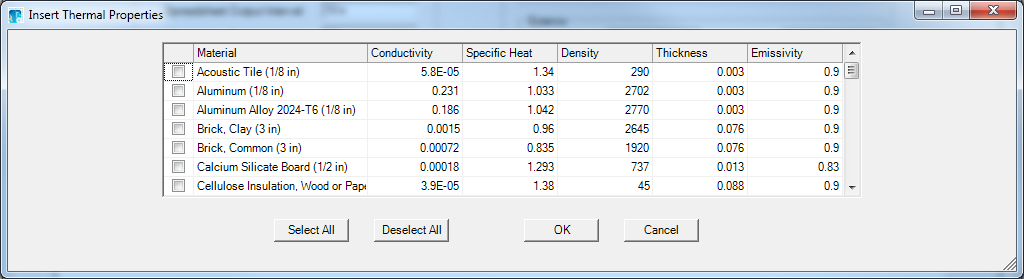
\includegraphics[width=6.5in]{FIGURES/Input_File/Insert_Thermal_Properties}
\end{center}
\end{figure}

To add additional thermal properties to a simulation or to edit existing ones, the \textbf{Edit Thermal Properties} menu item (see page \pageref{Thermal_Properties_Menu}) allows you to edit any of the existing thermal properties. \\~ \\

\begin{figure}[h!]
\begin{center}
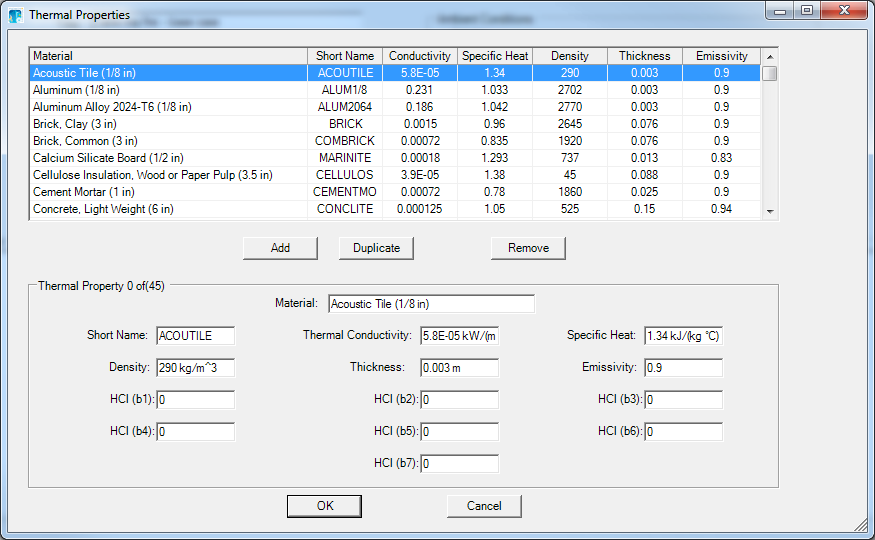
\includegraphics[width=6.5in]{FIGURES/Input_File/Edit_Thermal_Properties}
\end{center}
\end{figure}

\begin{description}
\item[Material] A descriptive name for the material.

\item[Short Name] A one-word (no more than 8 characters) \textbf{unique} identifier for the material.  This identifier should not contain any spaces and is used in other CFAST inputs to identify the particular material referenced.

\item[Thermal Conductivity] (default value: none, default units: kW/m \degc): Thermal conductivity for the material.

\item[Specific Heat] (default value: none, default units: kJ/kg \degc): Specific heat for the material.

\item[Density] (default value: none, default units: kg/m$^3$): Density for the material.

\item[Thickness] (default value: none, default units: m): Thickness of the material.  Note that if two materials with identical thermal properties but with different thicknesses aer desired, two separate materials must be defined.

\item[Emissivity] (default value: 0.9, default units: none): Emissivity of the material surface.  This is the fraction of radiation that is absorbed by the material.
\end{description}


\section{Modeling a Compartment as a Tall Shaft or Long Corridor}

For tall compartments or those removed from the room of fire origin, the compartment may be modeled as a single, well-mixed zone rather than the default two-zone assumption. A single zone approximation is appropriate for smoke flow far from a fire source, where the two-zone layer stratification is less pronounced than in compartments near the fire or in situations where the stratification does not occur. Examples are elevators, shafts, complex stairwells, or compartments far from the fire.

By specifying the compartment as a corridor, the ceiling jet temperature is calculated with a different empirical correlation that results in a somewhat higher temperature near the ceiling.  This will impact, for example, detectors, sprinkler, and targets near the ceiling in corridors.

\begin{description}
\item[Normal (Two-zone model)] Conditions in the compartment are calculated with the normal two-zone approach.

\item[Shaft (Single-zone model] Conditions in the compartment are calculated as single well-mixed zone.

\item[Corridor (Revised ceiling jet] Conditions in the compartment are calculated with the normal two-zone approach. Ceiling jet temperatures in the compartment are calculated with a revised empirical correlation specific to corridors.
\end{description}


\section{Defining Variable Compartment Area}

The Compartment Geometry page includes two additional entries that may be used for defining compartment properties for spaces which are not rectangular in area.  Values for a chosen compartment are entered in a spreadsheet.

\begin{description}
\item[Height Value(s)] (default units: m, default values: none): Values of height for the corresponding cross-sectional area values measured from the floor of the compartment. The values for the compartment correspond to cross-sectional area values included for the same compartment on the ROOMA command.

\item[Area Value(s)] (default units m$^2$, default values: none): Values of cross-sectional area of the compartment as a function of height measured from the floor of the compartment. The values for the compartment correspond to height values included for the same compartment on the ROOMH command.
\end{description}

\graybox{
Cross-sectional area values may vary larger or smaller with height as appropriate. \\

Overall compartment size (input with the COMPA command (see page \pageref{Compartment_Inputs}) must define a volume at least as large as the total volume of the compartment. Typically, the COMPA input can correspond to the largest area in the list of cross-sectional area values. \\

Once the total compartment volume is determined from the set of cross-sectional area and height inputs, an effective width and depth are calculated (maintaining the original user input for compartment height) so the compartment volume matches to actual total volume of the compartment. The aspect ratio (width/depth)is maintained. \\

Cross-sectional area values should be input in order by ascending height. If the first height value is not zero (i.e., at floor level), the cross-sectional area is assumed constant from the floor to the height specified in the first cross-sectional area value. \\

Similarly, if the last height value is not at the ceiling height, the cross-sectional area is assumed constant from the height specified in the last cross-sectional area value to the ceiling.
Between any two adjacent cross-sectional area data values in the input list, the area is assumed to be a pyramidal section (which by definition maintains the same width to depth aspect ratio for the compartment from floor to ceiling). \\

CFAST uses the variable cross-sectional area inputs to determine the layer height. The equations solved by CFAST determine the volume of the upper layer. For a normal rectangular room, this corresponds directly to a layer height. For a variable cross-sectional area compartment, a  numerical integration of the area inputs beginning at the ceiling is used to determine the height at which the upper layer occupies the calculated volume of the upper layer.
}



\chapter{Natural Ventilation}

Natural ventilation can occur when two compartments are connected via open doorways or windows (\textbf{Wall Vents}); or when two compartments are connected via \textbf{Floor/Ceiling Vents}. If no vents are specified between two compartments, they are assumed to be isolated.

\section{Wall Vents}

\begin{figure}[h!]
\begin{center}
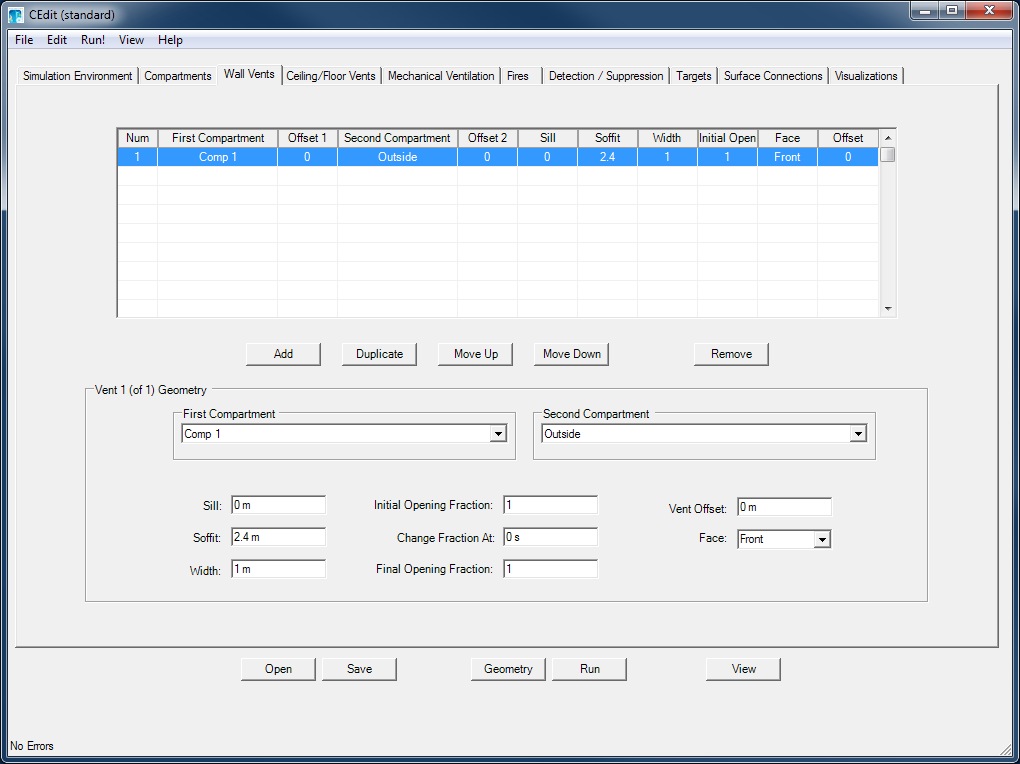
\includegraphics[width=6.5in]{FIGURES/Input_File/Natural_Flow_Tab}
\end{center}
\end{figure}

Wall vents can only be created between compartments that physically overlap in elevation at some point. These may include doors between compartments or windows in the compartments (between compartments or to the outdoors).  Openings to the outside are included as openings to a compartment with a number one greater than the number of compartments described in the geometry section. It is possible to define a total of 25 horizontal flow connections between any pair of compartments. Horizontal flow connections may also be used to account for leakage between compartments or to the outdoors.

\begin{description}
\item[First Compartment] First of the two compartments to be connected by a horizontal flow vent.  Compartments are numbered automatically by the input editor and by the model in the order they are read from the input data file and/or the order they appear in the summary table on the compartment geometry page. Compartment numbers begin with 1, so the first compartment is number 1, the second 2, and so forth.

\item[Second Compartment] Second of the two compartments to be connected by a horizontal flow vent.  Compartments are numbered automatically by the input editor and by the model in the order they are read from the input data file and/or the order they appear in the summary table on the compartment geometry page. Compartment numbers begin with 1, so the first compartment is number 1, the second 2, and so forth.

\item[Sill] (default units: m, default value: none): Sill height is the height of the bottom of the opening relative to the floor of the compartment selected as the first compartment.

\item[Soffit] (default units: m, default value: none): Position of the top of the opening relative to the floor of the compartment selected as the first compartment.

\item[Width] (default units: m, default value: none): The width of the opening.

\item[Initial Opening Fraction] (default value: 1): Flow through horizontal vents is calculated based on the area of the vent.  Normally, the vent is fully open.  If desired, the user may specify a fraction between 0 and 1 that allows the vent to be partially or fully closed at the beginning of the simulation.  In the model calculation, the vent width is multiplied by this fraction.  The opening fraction may be changed at any time in the simulation through the use of the EVENT command.

\item[Change Opening Fraction At Time]  (default units: s, default value: 0 s)  Time during the simulation at which to change the opening fraction.

\item[Final Opening Fraction] (default value: 1): for horizontal flow vents, the fraction specifies the fractional width opening of the vent. Fractional values must be between 0 and 1.

\item[Vent Offset] (default units: m, Default value: 0 m): For visualization, the vent offset is the horizontal distance between the near edge of this vent and the origin of the axis defined by the selected face(below) in the first compartment (Front and Rear are along the X-axis; left and right are along the Y-axis). For example, to place the vent at the center of the front wall, specify the front face at an offset of `compartment width/2 - vent width/2'.

\item[Face] For visualization, FACE specifies which wall the vent will be displayed on in Smokeview.  Choices are Front, Rear, Right, Left and are relative to the X-Z plane.
\end{description}

\graybox{
The soffit and sill specifications are with respect to the first compartment specified and are not necessarily symmetric since the elevation of the second compartment may be different than the first.  Reversing the order of the compartment designations can make a difference.
}

\section{Ceiling/Floor Vents}

\begin{figure}[h!]
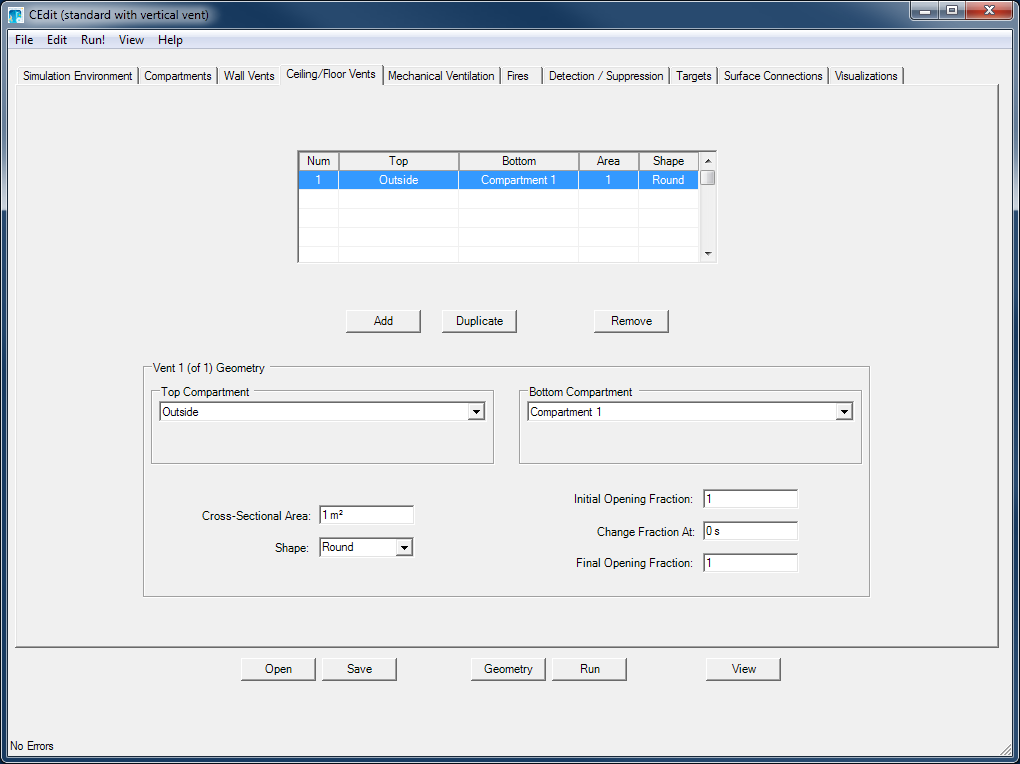
\includegraphics[width=6.5in]{FIGURES/Input_File/Vertical_Flow_Tab}
\end{figure}

This section of the input data file describes the inputs for natural flow vents in ceilings and floors. Examples of these openings are scuddles in a ship, or a hole in the roof of a residence. Combined buoyancy- and pressure-driven flow through a vertical flow vent is possible when the connected spaces adjacent to the vent are filled with gases of different density in an unstable configuration, with the density of the top space larger than that of the bottom space. With a moderate cross-vent pressure difference, the instability leads to a bi-directional flow between the two spaces. For relatively large cross-vent pressure difference the flow through the vent is unidirectional, from the high- to the low-pressure space.

Connections can exist between compartments or between a compartment and the outdoors. Openings to the outside are included as openings to a compartment with a number one greater than the number of compartments defined in the scenario. There are four parameters which include each of the connected compartments, the shape of the opening, and the effective area of the vent.

\begin{description}
\item[Top Compartment] The top or first of the two compartments to be connected by a vertical flow vent. The vent is through the floor of this compartment.  Compartments are numbered automatically by the input editor and by the model in the order that they are read from the input data file and/or the order they appear in the summary table on the compartment geometry page. Compartment numbers begin with 1, so the first compartment is number 1, the second 2, and so forth.

\item[Bottom Compartment] The bottom or second of the two compartments to be connected by a horizontal flow vent. The vent is through the ceiling of this compartment. Compartments are numbered automatically by the input editor and by the model in the order they are read from the input data file and/or the order they appear in the summary table on the compartment geometry page. Compartment numbers begin with 1, so the first compartment is number 1, the second 2, and so forth.

\item[Cross-sectional Area] (default units: m$^2$, default value: none): specifies the cross-sectional area of the vent connecting the two compartments.

\item[Shape] The shape factor is 1 for circular openings and 2 for square openings.

\item[Initial Opening Fraction] Flow through vertical vents is calculated based on the area of the vent.  Normally, the vent is fully open.  If desired, the user may specify a fraction between 0 and 1 that allows the vent to be partially or fully closed at the beginning of the simulation.  In the model calculation, the vent area is multiplied by this fraction.  The opening fraction may be changed at any time in the simulation through the use of the EVENT command.

\item[Change Opening Fraction At Time] (default units: s, default value: 0 s): Time during the simulation at which to change the opening fraction.

\item[Final Opening Fraction] for vertical flow vents, the fraction specifies the fractional cross-sectional area of the vent. Fractional values must be between 0 and 1.
\end{description}

\graybox{
Although obvious, note that the top or first compartment must be the compartment on top of the bottom or second compartment. \\

CFAST allows only a single connection between any pair of compartments included in a simulation. This limitation is based on the implementation of the vertical flow algorithm in CFAST and on the validation efforts for the original algorithm development  which only studied a single opening between connected compartments. \\

Vertical connections can only be created between compartments that could be physically stacked based on specified floor and ceiling elevations for the compartments.  Some overlap between the absolute floor height of one compartment and the absolute ceiling height of another compartment is allowed.  However, whether the compartments are stacked or overlap somewhat, the ceiling/floor absolute elevations must be within 0.01 m of each other. The check is not done when the connection is to the outside.
}


\chapter{Mechanical Ventilation}

\begin{figure}[h!]
\begin{center}
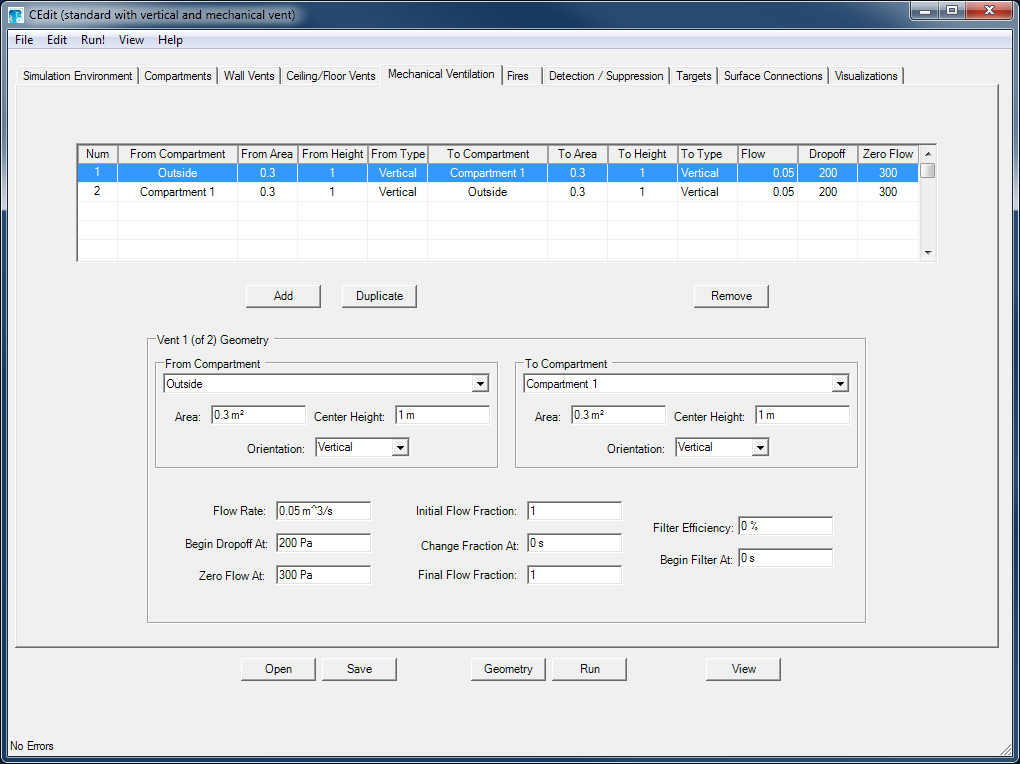
\includegraphics[width=6.5in]{FIGURES/Input_File/Mechanical_Vent_Tab}
\end{center}
\end{figure}

Fan-duct systems are commonly used in buildings for heating, ventilation, air conditioning, pressurization, and exhaust. Generally, systems that maintain comfortable conditions have either one or two fans.  Residences often have a systems with a single fan. Further information about these systems is presented in  Klote and Milke \cite{Klote:2002} and the American Society of Heating, Refrigerating and Air Conditioning Engineers \cite{ASHRAE:2001}.

The model for mechanical ventilation used in CFAST is based on the theory of networks and is based on the model developed by Klote \cite{Klote:1988a}.  This is a simplified form of Kirchoff's law which says that flow into a node must be balanced by flow out of the node. The equations used describe the relationship between the pressure drop across a duct, the resistance of a duct, and the mass flow.  The pressure can be changed by conditions in a compartment, or a fan in line in the duct system.  Resistance arises from the finite size of ducts, roughness on duct surfaces, bends and joints. In CFAST, default values are used for the duct properties, and thus mechanical ventilation connections are simply described by the connections to the two compartments and a fan whose throughput is a constant volumetric flow up to a user-specified pressure drop across the fan, dropping to zero at high backwards pressure on the fan.

\section{Connections to Compartments}

\begin{description}
\item[From Compartment] The first compartment to which the mechanical ventilation system diffuser is connected. Fan flow is from this compartment.  Compartments are numbered automatically by the input editor and by the model in the order they are read from the input data file and/or the order they appear in the summary table on the compartment geometry page. Compartment numbers begin with 1, so the first compartment is number 1, the second 2, and so forth.

\item[From Compartment Area] (default units: m$^2$, default value: none): Cross-sectional area of the opening into the compartment. The area will be truncated if the midpoint (height) is set such that the height plus or minus the effective length is above the compartment ceiling or below the floor.

\item[From Compartment Height] (default units: m, default value: none): Height of the duct opening above the floor of the compartment measured from the midpoint of the register.

\item[From Compartment Orientation] The orientation of the diffuser relative to the floor of the compartment.  A horizontal diffuser implies vertical flow through the ceiling or floor of the compartment.  A vertical diffuser implies horizontal flow through a wall of the compartment.

\item[To Compartment] The bottom or second of the two compartments to be connected by a horizontal flow vent. The vent is through the ceiling of this compartment. Compartments are numbered automatically by the input editor and by the model in the order they are read from the input data file and/or the order they appear in the summary table on the compartment geometry page. Compartment numbers begin with 1, so the first compartment is number 1, the second 2, and so forth.

\item[To Compartment Area] (default units: m$^2$, default value: none): Cross-sectional area of the opening into the compartment. The area will be truncated if the midpoint (height) is set such that the height plus or minus the effective length is above the compartment ceiling or below the floor.

\item[To Compartment Height] (default units: m, default value: none): Height of the duct opening above the floor of the compartment measured from the midpoint of the register.

\item[To Compartment Orientation] The orientation of the diffuser relative to the floor of the compartment.  A horizontal diffuser implies vertical flow through the ceiling or floor of the compartment.  A vertical diffuser implies horizontal flow through a wall of the compartment.
\end{description}

\section{Fans}

\begin{description}
\item[Flow Rate] (default units: m$^3$/s, default value: none): Constant flow rate of the forced-air flow from the first compartment to the second compartment.

\item[Begin Drop Off Pressure] (default units: Pa, default value: 200 Pa): The description of the fan includes a drop off in flow beginning at a pressure specified by the user.  Above this pressure drop, the flow gradually drops to zero flow.

\item[Zero Flow Pressure] (default units: Pa, default value: 300 Pa): Specifies the pressure above which the flow through the mechanical ventilation connection is zero.

\item[Initial Opening Fraction] Flow through mechanical vents is calculated based on the area of the vent.  Normally, the vent is fully open.  If desired, the user may specify a fraction between 0 and 1 that allows the vent to be partially or fully closed at the beginning of the simulation.  In the model calculation, the fan flow rate is multiplied by this fraction.  The opening fraction may be changed at any time in the simulation through the use of the EVENT command.

\item[Change Opening Fraction At Time] (default units: s, default value: none): Time during the simulation at which to change the opening fraction.

\item[Final Opening Fraction] for mechanical flow vents, the fraction specifies the fractional fan flow rate for the vent. Fractional values must be between 0 and 1.
\end{description}

\graybox{
CFAST does not include provisions for reverse flow through a fan. Calibration for backward flow is not provided by fan manufacturers, so the equations incorporated in CFAST do not allow for such flow. The problem is simply that in this flow regime, the fan has stalled, and likely will soon fail. \\

If the simulation includes mechanical ventilation filtering, care should be taken in choosing trace species production rates to insure the production rate is small compared to the total pyrolysis rate.  This will allow appropriate conservation of mass in the solution of the system of differential equation.  For large production rates of trace species, scaling factors can be used (e.g., divide by 1000) for the trace species production rate to reduce the relative magnitude compared to the pyrolysis rate.  For analysis, the resulting trace species in compartments and filters can be converted back to original units multiplying by the scaling factor used.
}

\section{Filtering}

For mechanical vents, there are two species that can be filtered out of the gas flow: soot and the user-defined trace species. Filters are applied only to fan openings. The fan must have been defined before the filter can be applied. Initially filtering is off. It is turned on with the EVENT key word, defined in the input editor with a Filter Efficiency and Begin Filter At time.

\begin{description}
\item[Filter Efficiency] (default units:~\%, default value: none): Flow through mechanical vents may include filtering that removes a user-specified portion of soot and trace species mass from the flow through the vent.  By default, there is no filtering applied, that is all of the soot and trace species mass in the vent flow is passed through the vent. Within the user interface, this is specified as a filter efficiency of 0~\%.  If desired, the user may specify the fraction of the soot and trace species mass to be removed as a percentage.

\item[Begin Filtering At Time] (default units: s, default value: none): Time during the simulation at which the mechanical vent filtering begins.
\end{description}

\graybox{
If the simulation includes mechanical ventilation filtering, care should be taken in choosing trace species production rates to insure the production rate is small compared to the total pyrolysis rate.  This will allow appropriate conservation of mass in the solution of the system of differential equation.  For large production rates of trace species, scaling factors can be used (e.g., divide by 1000) for the trace species production rate to reduce the relative magnitude compared to the pyrolysis rate.  For analysis, the resulting trace species in compartments and filters can be converted back to original units multiplying by the scaling factor used.
}



\chapter{Fires}

A simulated fire in CFAST is implemented as a source of fuel mass which is released at a prescribed rate (the pyrolysis rate). Energy is released by the fuel and combustion products are created as it burns. In the fire, species production is calculated based on production yields prescribed by the user. In addition, the pyrolysis rate and resulting energy and species generation may be limited by the oxygen available for combustion. When sufficient oxygen is available for combustion, the heat release rate for the constrained fire is the same as for the unconstrained fire.

The model can simulate multiple fires in one or more compartments of the building.  These fires are treated as totally separate entities, with no interaction of the plumes. These fires are generally referred to as “objects” and can be ignited at a prescribed time, temperature or heat flux.

CFAST does not include a pyrolysis model to predict fire growth. Rather, pyrolysis rates for each fire are prescribed by the user.  While this approach does not directly account for increased pyrolysis due to radiative feedback from the flame or compartment, in theory these effects could be prescribed by the user as described in this section.  In an actual fire, this is an important consideration, and the specification used should consider the experimental conditions as closely as possible.

A fire releases energy based on the pyrolysis of fuel, but may be constrained by the oxygen available for combustion depending on the compartment conditions. Complete burning will take place only where there is sufficient oxygen.  When insufficient oxygen is entrained into the fire plume, unburned fuel will be transported from zone to zone until there is sufficient oxygen and a high enough temperature to support combustion.  In general, CFAST uses a simple definition of a combustion reaction that includes major products of combustion for hydrocarbon fuels:

\begin{eqnarray}
   \mathrm{C_{n_\C}H_{n_H}O_{n_O}N_{n_N}Cl_{n_{Cl}}} &+&  \nu_\OTWO \, \mathrm{O_2}  \rightarrow  \nonumber \\[.1in]
   \nu_\COTWO \, \mathrm{CO_2} &+& \nu_\HTWOO \, \mathrm{H_2O} \; + \; \nu_\CO \, \mathrm{CO} \; + \; \nu_\So \, \mathrm{Soot} \; + \; \nu_\HCl \mathrm{HCl} \; + \; \nu_\HCN \mathrm{HCN} \label{stoich}
\end{eqnarray} \\
assuming that all the nitrogen and chlorine in the fuel are converted to HCN and HCl. The stoichiometric coefficients $\nu_\So$, $\nu_\CO$, etc. represent appropriate molar ratios for a stoichiometric balance of the equation. For complete combustion of the simplest hydrocarbon fuel, methane reacts with oxygen to form carbon dioxide and water. The only inputs required are the fuel composition, heat release rate, and heat of combustion. For fuels that contain oxygen, nitrogen, or chlorine, the reaction becomes more complex. Stoichiometry is used to insure conservation of mass and elements in the reaction. The species which are calculated are oxygen, carbon dioxide, carbon monoxide, water, total unburned fuel (tuhc), and soot. Gaseous nitrogen is included, but only acts as a diluent.

\begin{figure}[h!]
\begin{center}
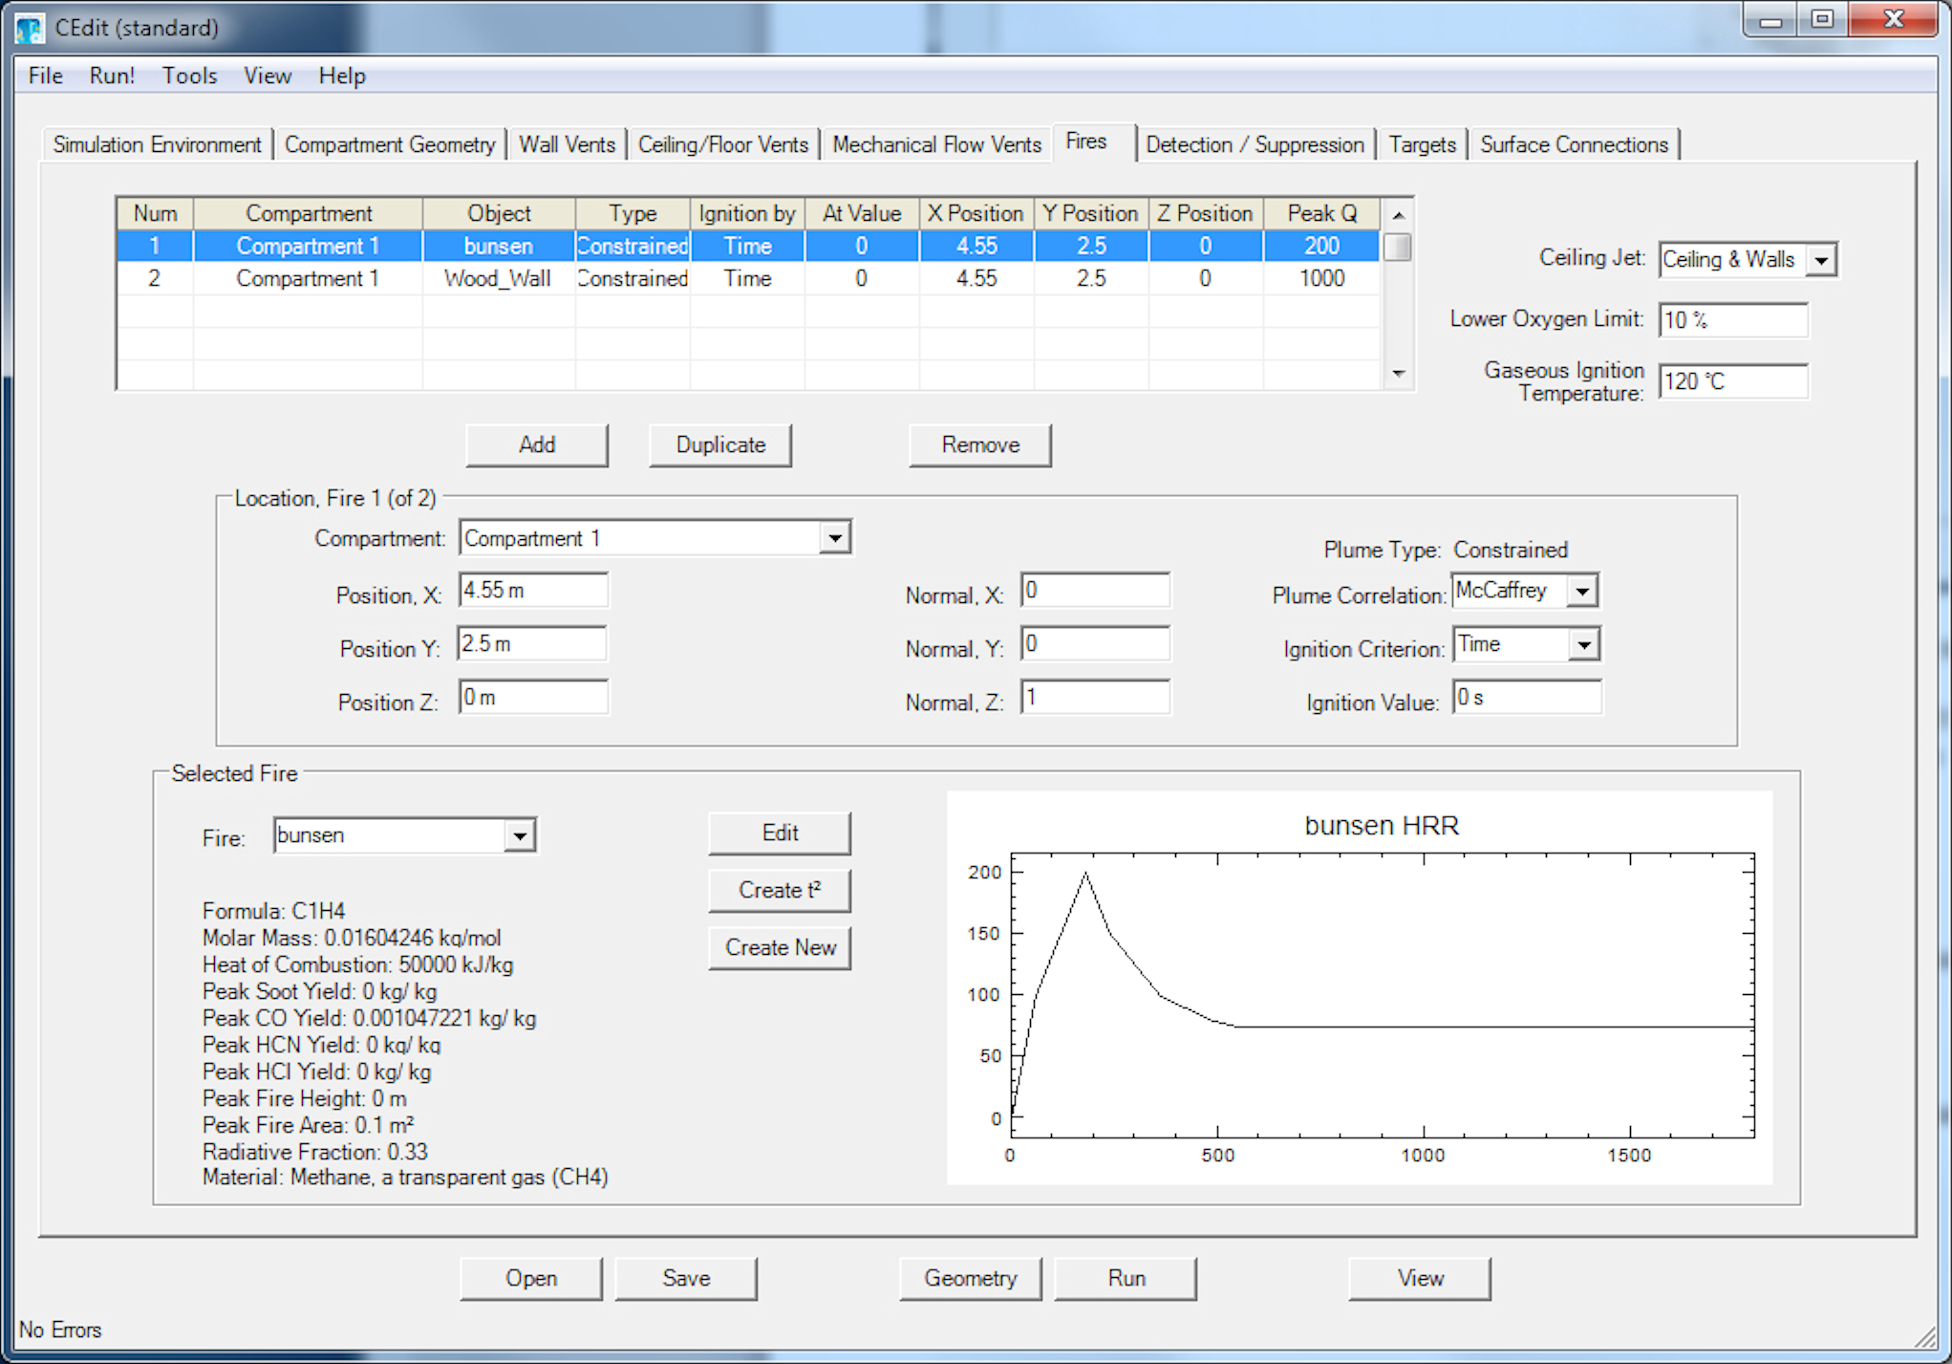
\includegraphics[width=6.5in]{FIGURES/Input_File/Fire_Tab}
\end{center}
\end{figure}

Two inputs on the Fire Tab are global, that is, they apply to all fires included in a simulation.
\begin{description}
\item[Lower Oxygen Limit] (default units: \%, default value: 10~\%):  In the CFAST model, a limit is incorporated by limiting the burning rate as the oxygen level decreases until a ``lower oxygen limit'' (LOL) is reached. The lower oxygen limit is incorporated through a smooth decrease in the burning rate near the limit. Normally, this value would not be changed by the user.

\item[Gaseous Ignition Temperature] (default units: \degc, default value: ambient temperature plus 100 K): The lower temperature limit on the burning of fuel in a gas layer. Since CFAST does not support a combustion kinetics model, this is the algorithm used for fires out of vents.  Normally, this value would not be changed by the user.
\end{description}

\section{Defining Individual Fires}

Fires in CFAST are defined as a series of individual fire objects which are then placed as desired in compartments in a simulation.

Each fire object defines the time dependent variables of the fire described by the mass loss rate, rate of heat release, fuel height, and fuel area.  Species production rates are specified in a manner similar to the fire, entering the rates as a series of points with respect to time.  The species which are followed by CFAST are: carbon dioxide, carbon monoxide, hydrogen cyanide, hydrogen chloride, nitrogen, oxygen, soot, total unburned hydrocarbons and water. There is a separate calculation of the concentration-time product Ct. Finally, a user-specified trace species can be specified to follow the transport that results from fire-induced flow for an arbitrary species. This may be of particular interest for radiological releases \cite{Jones:2008}, but may be useful for any trace amounts released by a fire.

Each fire object is defined in a separate comma-separated spreadsheet file with an extension of ``.o'' and is also saved in the CFAST input file for the current simulation. A pull-down allows the user to select one of the predefined fire objects to place in the chosen compartment. As many fire objects as desired may be defined by the user.  At least one fire in the simulation should ignite at a user-specified time.  Other fire objects can ignite based on time, temperature or heat flux conditions.

\begin{figure}[h!]
\begin{center}
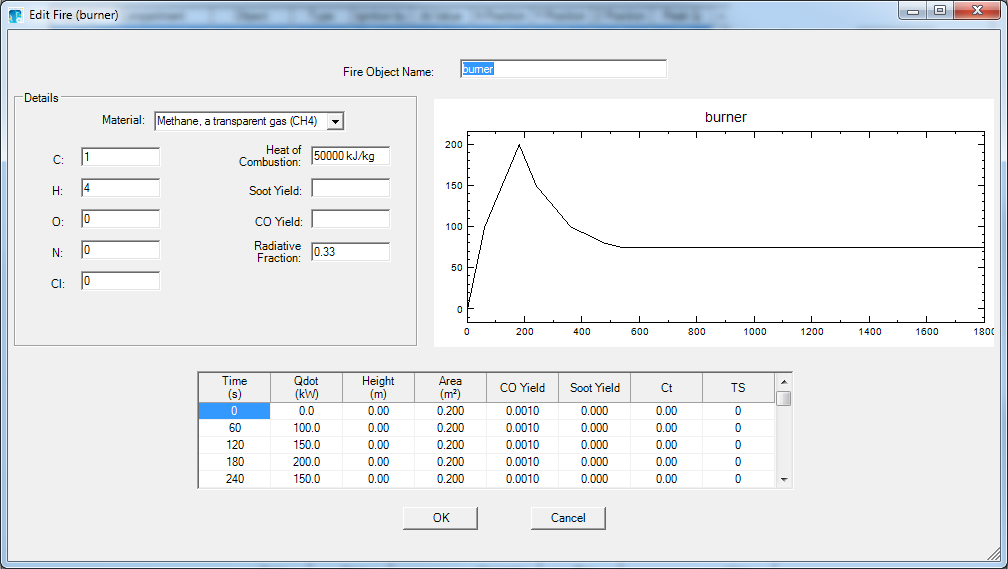
\includegraphics[width=6.5in]{FIGURES/Input_File/Fire_Object_Edit}
\end{center}
\end{figure}

\begin{description}
\item[Fire Object Name] The name for the desired object.  This also corresponds to the name of the fire object file, without the extension. The selected name must be unique (i.e., not the same as another fire object in the same simulation).

\item[Material] (default value: none): material name from the list of thermal properties used for the object. The material properties are used to calculate heat transfer into the object from its surroundings.

\item[C, H, O, N, Cl] Molecular formula of the burning fuel. Burning fuels in CFAST are assumed to be hydrocarbon fuels that contain at least Carbon and Hydrogen and optionally Oxygen, Nitrogen, and Chlorine. These five inputs define the stoichiometry of the fuel as it is burned.  Thus, for example, all of the specified Nitrogen and Chlorine is assumed to completely react to form HCN and HCl.  If only partial conversion is desired, a smaller ratio for Nitrogen and/or Chlorine can be specified.

\item[Heat of Combustion] (default units: J/kg, default value: 50 000 000 J/kg): The energy released per kilogram of mass burned.

\item[Soot Yield] (default units: kg/kg, default value: 0 kg/kg): Constant species yields of soot expressed as ratios of carbon to fuel produced by the pyrolysis of the fuel. This input allows the user to specify a single value for soot yield for all time points in the fire time line. Individual time points can be changed as desired in the spreadsheet input described below.

\item[CO Yield] (default units: kg/kg, default value: determined by correlation): Constant species yield of carbon monoxide expressed as a fraction of the fuel mass converted into carbon monoxide.  By default, the CO yield is related to the soot yield via the correlation developed by K\"oyl\"u and Faeth

\be
y_{CO} = \frac{12n_C}{M_fv_f}0.0014 + 0.37y_s \label{eq:Koylu}
\ee
where $n_C$ is the number of carbon atoms in a fuel molecule, $M_f$ is the molecular weight of the fuel, and $v_f$ is the stoichiometric coefficient of the fuel, assumed to be 1 here \cite{Koylu:1991}. Note that this correlation refers to well-ventilated fires. Yields of CO and soot in under-ventilated fires is still a subject of active research.

\item[Radiative Fraction] The fraction of the energy produced in combustion that is radiated from the fire and plume. Within CFAST, the radiative fraction defaults to 0.35 ; i.e., 35 \% of the fire’s energy is released via radiation.  For other fuels, the work of Tewarson \cite{Tewarson:2003}, McCaffrey \cite{McCaffrey:1982}, or Koseki \cite{Koseki:1989} is available for reference.  The typical range for the radiative fraction is from about 0.05 to 0.4.
\end{description}

For all fires, including t-squared fires, values are calculated for time dependent variables, including default values for species generation. For all inputs, these values can be changed. All of the time dependent variables depend on a predefined time line. The time input specifies a sequence of time points that define the timing of the fire.  An entry indicates a point on the time-line when the mass loss rate, fuel height and other time dependent values are specified for the fire.  This time is independent of the simulation time which is specified by the TIMES line. If the simulation time is longer than the total duration of the fire, the final values specified for the fire (mass loss rate, fuel height, fuel area, and species) are continued until the end of the simulation.

\begin{description}
\item[Time] (default units: s, default values: none): specify a sequence of time points that define the timing of the main fire.  An entry indicates a point on the time-line when the heat release loss rate, fuel height and other time dependent values are specified for the fire.

\item[Heat Release Rate (Qdot)] (default units: kW, default values: none): Heat release rate of the fire as a series of time points consistent with the time specification.

\item[Fire Height] (default units: m, default values: 0 m): Time-based values for height of the base of the fire.  Actual height of the base of the fire is the sum of the constant value specified for the fire and this height specification for a particular time in the fire development.

\item[Area] of the Base of the Fire (default units: m$^2$, default values: 0.3 m$^2$): Cross-sectional area of the base of the fire.

\item[CO Yield] (default units: kg/kg, default values: constant value from correlation, in eq. \ref{eq:Koylu}): yield of carbon monoxide expressed as a fraction of the fuel mass converted into carbon monoxide.

\item[Soot Yield] (default units kg/kg, default values: none): yield of soot expressed as a fraction of fuel mass converted into smoke particulate..

\item[Ct] (default units: kg/kg, default values: none): Yield of a fictitious toxic species per mass of fuel produced in the pyrolysis of the fuel.

\item[TS] (default units: kg/kg, default values: none): Yield of user-defined trace species per mass of fuel produced in the pyrolysis of the fuel.
\end{description}

\graybox{

Production of hydrogen cyanide and hydrogen chloride are tracked solely based on user prescribed yields. \\

The heat release rate for a constrained fire may be reduced below its prescribed value based upon the oxygen available for combustion. For the constrained fire, the burning rate may be less than the pyrolysis rate and cannot be simplified as in the case of the unconstrained fire. As fuel and oxygen are consumed, heat is released and various products of combustion are formed. \\

For a constrained fire, the heat release rate is limited by available oxygen. This limit is applied in three places: The first is burning in the portion of the plume which is in the lower layer of the room of fire origin; the second is the portion of the plume in the upper layer, also in the room of origin; the third is in the vent flow which entrains air from a lower layer into an upper layer in an adjacent compartment. The unburned fuel is tracked in this model. Combustion of CO to CO$_2$ is not included in the model. Detailed combustion chemistry is not considered in CFAST due to the complexities associated with detailed kinetics and transport. \\

There are two calculations involving radiation in this model. One is for the overall energy balance and is based on broadband radiation absorption. The amount of radiation absorbed is sensitive to the species present, specifically water vapor, soot and carbon dioxide. The other is for visibility of egress signs. This calculation is based solely on the soot volume fraction and is reported as optical depth (per meter). The conversion factor is based on the recent work by Mulholland and Croarkin \cite{Mullholland:2000}. The value for converting mass density in kg/m3 to optical depth is 3817 m$^2$/kg. The value reported is intended specifically for assessing the visibility of egress signs, based on the work of Jin \cite{Jin:1979}.  It is not applicable to the far blue or red regions of the spectrum and so should not be used for assessing optical detection of fires through smoke. \\

With the two parameters, heat of combustion ($H_C$) and heat release rate $\dQ$, the pyrolysis rate of the fuel is determined by $\dm=\frac{\dQ}{H_C}$. \\

By default, the fire is placed in the center of the compartment on the floor.  If values for any of the three variables are invalid (i.e., less than zero or greater than the compartment dimension in the appropriate direction), the location for that direction defaults to the center of the appropriate direction in the width or depth direction and at the floor for the vertical direction. \\

The area of the base of the fire should not be left at a value of zero. Radiation from the fire is determined by a point source calculation from the vertical center of the flame which is in turned determined by Heskestad's flame height correlation \cite{Heskestad:2002}, a function of heat release rate and fire area. \\

For “normally toxic” materials, Ct takes a value of 1 and is typically changed by an order of magnitude for particularly toxic or non-toxic materials.  It is not part of the mass balance for the fuel and system, but it just carried along as a transported species in flow through the structure. Ct is used as a measure of toxicity of a material.  Typically the integrated Ct versus time product is calculated. For normal materials, a concentration-time product of 900 mg min/m$^3$ is an indication of incapacitation. \\

The trace species is transported along with fire gases, but is assumed not to take part in the combustion reaction and is assumed not to be a significant source of overall mass for the system mass balance calculated by the model. This implies that the production rate of trace species specified should be much smaller than the total specified pyrolysis rate. If necessary, the trace species can be scaled to a smaller value (e.g., divided by 1000) for the simulation and converted back for analysis (e.g., multiplied by 1000). \\

In the input editor, time-dependent data are entered in a simple spreadsheet. Normal windows copy (Ctrl-C), cut (Ctrl-X), and paste (Ctrl-V) keyboard shortcuts are available for data editing. In addition, Alt-Ins will insert a complete row above the currently-selected row in the spreadsheet and Alt-Del will delete the current row in the spreadsheet.
}

\subsection{Adding and Editing Fires}

By default, CEdit does not include predefined fires. Thus, the user needs to define fire objects for use with a specific simulation.  These may be from other simulations or input directly from reference sources or test results. The \textbf{Insert Fires} Menu item (see page \pageref{Fires_Menu}) allows you to add fires from an existing data file to the current simulation.

\begin{figure}[h!]
\begin{center}
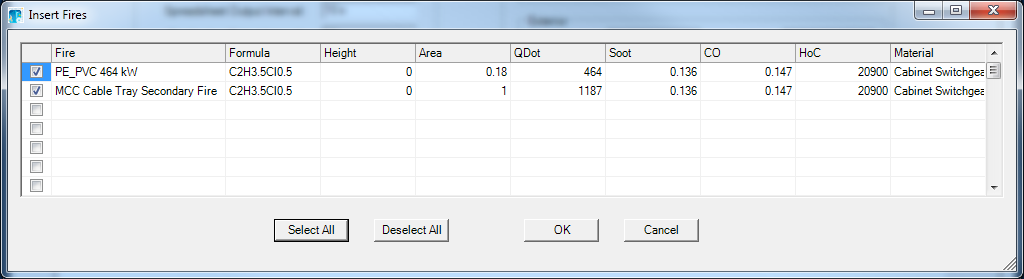
\includegraphics[width=6.5in]{FIGURES/Input_File/Insert_Fire_Objects}
\end{center}
\end{figure}

\subsection{T-squared Fires}

Use the Create t$^2$ button to create a new fire object with a heat release rate specified by the user in the form of a t-squared fire.  For a wide range of fires, the fire growth can be accurately represented with a power law relation of the form $\dQ=\alpha t^2$  where $\dQ$  is the heat release rate of the fire, $\alpha$ is the fire intensity coefficient, and $t$ is time \cite{Schifiliti:2002}. A set of specific t-squared fires labeled slow, medium, and fast, with fire intensity coefficients ($\alpha$) such that the fires reached 1054 kW (1000~BTU/s) in 600~s, 300~s, and 150~s, respectively were proposed for design of fire detection systems .  Later, these specific growth curves and a fourth called "Ultra-fast" which reaches 1054~kW in 75~s, gained favor in general fire protection applications. A separate window allows the user to define the t-squared fire. Details of the inputs for a t-squared fire is included below.

\begin{figure}[h!]
\begin{center}
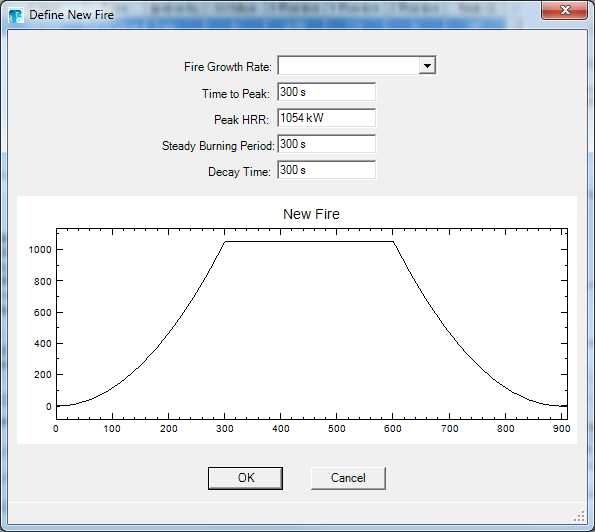
\includegraphics[width=5in]{FIGURES/Input_File/Create_t2}
\end{center}
\end{figure}

\begin{description}
\item[Fire Growth Rate] A set of specific t-squared fires labeled slow, medium, fast, or ultra-fast with fire intensity coefficients ($\alpha$) such that the fires reached 1054~kW (1000~BTU/s) in 600~s, 300~s, 150~s, and 75~s are available.  Each of these growth rates (with corresponding decay rates) can be selected. A fifth, custom, selection allows the user to define any growth or decay rate desired.

\item[Time to Peak] (default units: s, default value: 300 s): The time for the fire to reach the peak fire size.

\item[Peak HRR] (default units: kW, default value: 1054 kW): The peak heat release rate of the t-squared fire.  Fire size is constant beginning at a time consistent with the time to reach the peak value,   and continues at that value for the time specified in the steady burning period, below.

\item[Steady Burning Period] (default units: s, default value: 300 s): Duration of time that the fire continues burning at the rate specified by the maximum HRR input, above.

\item[Decay Period] (default units: s, default value, 300 s): Duration of time for the fire to decay back to a zero value.  Decay follows the inverse of the t-squared growth rate.
\end{description}

\section{Fire Location}

Fires  are placed in defined positions within a compartment of a simulation and oriented with a normal vector to the surface of the object.  Ignition of an object may be at a specified time, a specified net incident heat flux on the surface of the object, or at a specified surface temperature of the object.

\begin{description}
\item[Compartment] of Fire Origin: specifies the compartment that contains the main fire for the simulation.  Any compartment defined is valid.

\item[Position X] (default units: m, default value: compartment width / 2): Position of the center of the base of the fire measured in the x direction from the front lower left corner of the compartment origin (0,0,0) in the compartment of fire origin.

\item[Position Y] (default units: m, default value: compartment depth / 2): Position of the center of the base of the fire measured in the y direction from the front lower left corner of the compartment origin (0,0,0) in the compartment of fire origin.

\item[Position Z] (default units: m, default value: 0 m): Position of the center of the base of the fire measured in the z direction from the front lower left corner of the compartment origin (0,0,0) in the compartment of fire origin. Actual height of the base of the fire is the sum of the value specified by FPOS and by FHIGH for a particular time in the fire development.

\item[Normal  X] Component: specifies a vector of unit length perpendicular to the exposed surface of the object. (Depth) component is in the direction from the rear wall of the object compartment. Default value is a horizontal, upward facing object, unit vector = (0,0,1)

\item[Normal  Y] Component: specifies a vector of unit length perpendicular to the exposed surface of the object. (Breadth) component is in the direction from the left wall of the object compartment. Default value is a horizontal, upward facing object, unit vector = (0,0,1)

\item[Normal  Z] Component: specifies a vector of unit length perpendicular to the exposed surface of the object. (Breadth) component is in the direction from the floor of the object compartment. Default value is a horizontal, upward facing object, unit vector = (0,0,1)

\item[Ignition Criterion] The type of ignition condition specified by the Ignition Criterion Value. Acceptable values are 1 for time, 2 for object surface temperature, and 3 for incident flux to object surface.

\item[Ignition Value] The numerical value at which ignition will occur. If it is less than or equal to zero, the default value of zero is taken.
\end{description}

\section{Calculating Normal Vectors}

The general equations for determining the normal vectors in the x, y, and z directions are \\~

Normal vector in the x direction, $x = \sfrac{x}{\sqrt{x^2 + y^2 + z^2}}$ \\

Normal vector in the y direction, $y = \sfrac{y}{\sqrt{x^2 + y^2 + z^2}}$ \\

Normal vector in the z direction, $z = \sfrac{z}{\sqrt{x^2 + y^2 + z^2}}$ \\

The simplest way to calculate the unit vector is to draw an imaginary line at right angles (i.e., 90$^\circ$ angle) from the exposed surface of the target and to extend this imaginary line until it hits the walls, floor or ceiling of the compartment in which it is located.  This imaginary line is actually a vector that starts at the surface of the exposed target and terminates on a wall, floor, or ceiling.  Once the start point and the end point of a vector are known, the unit vector for this imaginary line may be calculated as follows:

\begin{equation}
  \begin{aligned}
 x &= \sfrac{x_{end} - x_{start}}{\sqrt{\brackets{x_{end} - x_{start}}^2 + \brackets{y_{end} - y_{start}}^2 + {z_{end} - z_{start}}^2}} \\
 y &= \sfrac{y_{end} - y_{start}}{\sqrt{\brackets{x_{end} - x_{start}}^2 + \brackets{y_{end} - y_{start}}^2 + {z_{end} - z_{start}}^2}} \\
 z &= \sfrac{z_{end} - z_{start}}{\sqrt{\brackets{x_{end} - x_{start}}^2 + \brackets{y_{end} - y_{start}}^2 + {z_{end} - z_{start}}^2}}
  \end{aligned}
\end{equation}

As an example, assume the following scenario:

\begin{itemize}
\item A square shaped target object is located in the middle of the floor of a compartment.
\item The target is constructed from non-combustible materials except the top.
\item The square shaped material is 1 m in depth, 1 m in breadth, and 1 m high.
\item The reference point (0,0,0) in the compartment is the lower left hand side of the rear wall.
\item The compartment is 3 meters in the x direction (i.e., the distance from the rear wall to the front wall of the compartment), 4 meters in the y direction (i.e., the distance from the left wall to the right wall of the compartment), and 5 meters in the z direction (i.e., the distance from the floor to the ceiling of the compartment).
\end{itemize}

Since the only side of the target that is combustible is the top surface of the target object, an imaginary line is draw perpendicular (i.e., at a 90$^\circ$ angle) from the top surface of the target object and extended until it reaches the outer boundary of the compartment.  In this case, since the top of the target object is facing the ceiling, the imaginary line would run straight up to the ceiling, running parallel to the four walls of the compartment, and terminating at the ceiling at the point (1.5 m, 2 m, 5 m).  Since the vector starts at point (1.5-m, 2-m, 1-m) and terminates at (1.5-m, 2-m, 5-m), the unit vectors can be calculated as follows:


\begin{equation}
  \begin{aligned}
 x &= \sfrac{x_{end} - x_{start}}{\sqrt{\brackets{x_{end} - x_{start}}^2 + \brackets{y_{end} - y_{start}}^2 + {z_{end} - z_{start}}^2}} &= \sfrac{1.5 - 1.5}{\sqrt{\brackets{1.5 - 1.5}^2 + \brackets{2 - 2}^2 + {5 - 1}^2}} \\
 y &= \sfrac{y_{end} - y_{start}}{\sqrt{\brackets{x_{end} - x_{start}}^2 + \brackets{y_{end} - y_{start}}^2 + {z_{end} - z_{start}}^2}} &= \sfrac{2 - 2}{\sqrt{\brackets{1.5 - 1.5}^2 + \brackets{2 - 2}^2 + {5 - 1}^2}} \\
 z &= \sfrac{z_{end} - z_{start}}{\sqrt{\brackets{x_{end} - x_{start}}^2 + \brackets{y_{end} - y_{start}}^2 + {z_{end} - z_{start}}^2}}  &= \sfrac{5 - 1}{\sqrt{\brackets{1.5 - 1.5}^2 + \brackets{2 - 2}^2 + {5 - 1}^2}} \\
  \end{aligned}
\end{equation}

In this case, the unit vector in the +Z direction.



\chapter{Sprinklers and Detectors}

Sprinklers and detectors are both considered detection devices by the CFAST model and are handled using the same inputs.  Detection is based upon heat transfer to the detector. Fire suppression by a user-specified water spray begins once the associated detection device is activated.

\begin{figure}[h!]
\begin{center}
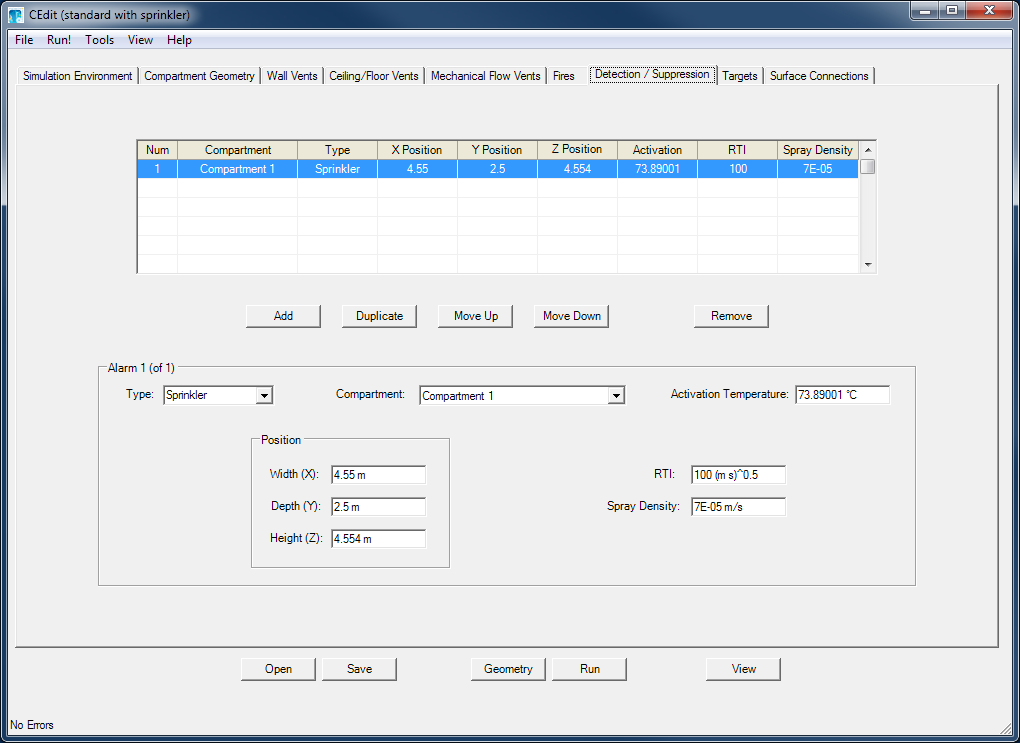
\includegraphics[width=6.5in]{FIGURES/Input_File/Detector_Tab}
\end{center}
\end{figure}

\begin{description}
\item[Type] type of detector, select smoke detector, heat detector, or sprinkler.

\item[Compartment] the compartment in which the detector or sprinkler is located.

\item[Activation Temperature] (default units: \degc, default value: dependent on type): the temperature at or above which the detector link activates.

\item[Width (X)] Position (default units: m, default value: none): position of the object as a distance from the left wall of the compartment (X direction).

\item[Depth (Y)] Position (default units: m, default value: none): position of the detector or sprinkler as a distance from the front wall of the compartment (Y direction).

\item[Height (Z)] Position (default units: m, default value: none): position of the object as a distance from the floor of the compartment (Z direction).

\item[RTI] (default units: (m$\cdot$s)$^{1/2}$, default value: none): the Response Time Index (RTI) for the sprinkler or detection device.

\item[Spray Density] (default units: m/s, default value: none): the amount of water dispersed by a sprinkler.  The units for spray density are length/time, derived by dividing the volumetric flow rate by the spray area. The suppression calculation is based upon an experimental correlation by Evans~\cite{Evans:1993}.
\end{description}

\graybox{
Often, the activation of smoke alarms is simulated with a temperature-based criterion, typically in the range of 5~\degc to 10~\degc above ambient. Davis and Notarianni  studied the activation of heat and smoke alarms in small and large compartments \cite{Davis:1996}. They conclude that a temperature rise of approximately 5~\degc corresponded to activation of ionization alarms for a range of fire sources and ceiling heights. The Nuclear Regulatory Commission includes a default value of 10~\degc in NUREG-1805 \cite{NRCNUREG1805}. \\

Several cautions should be observed when using estimates of sprinkler suppression within the model: 1) the first sprinkler activated controls the effect of the sprinkler on the heat release rate of the fire.  Subsequent sprinklers which may activate have no additional effect on the fire simulation. 2) The fire suppression algorithm assumes the effect of the sprinkler is solely to reduce the heat release rate of the fire. Any effects of the sprinkler spray on gas temperatures or mixing within the compartment are ignored. 3) The sprinkler always reduces the heat release rate of the fire. The ability of a fire to overwhelm an under-designed sprinkler is not modeled. 4) Since the dynamics of the sprinkler and direct effects of the spray on gas temperatures and velocities are not modeled, calculated times of activation of secondary sprinklers and / or detectors after the first sprinkler is activated should be not be modeled since the impact of the first sprinkler on the activation of additional sprinklers is not included in the CFAST model.
}



\chapter{Defining Targets}

CFAST can track and report calculations of the net heat flux striking arbitrarily positioned and oriented targets and the temperature of these targets.

\begin{figure}[h!]
\begin{center}
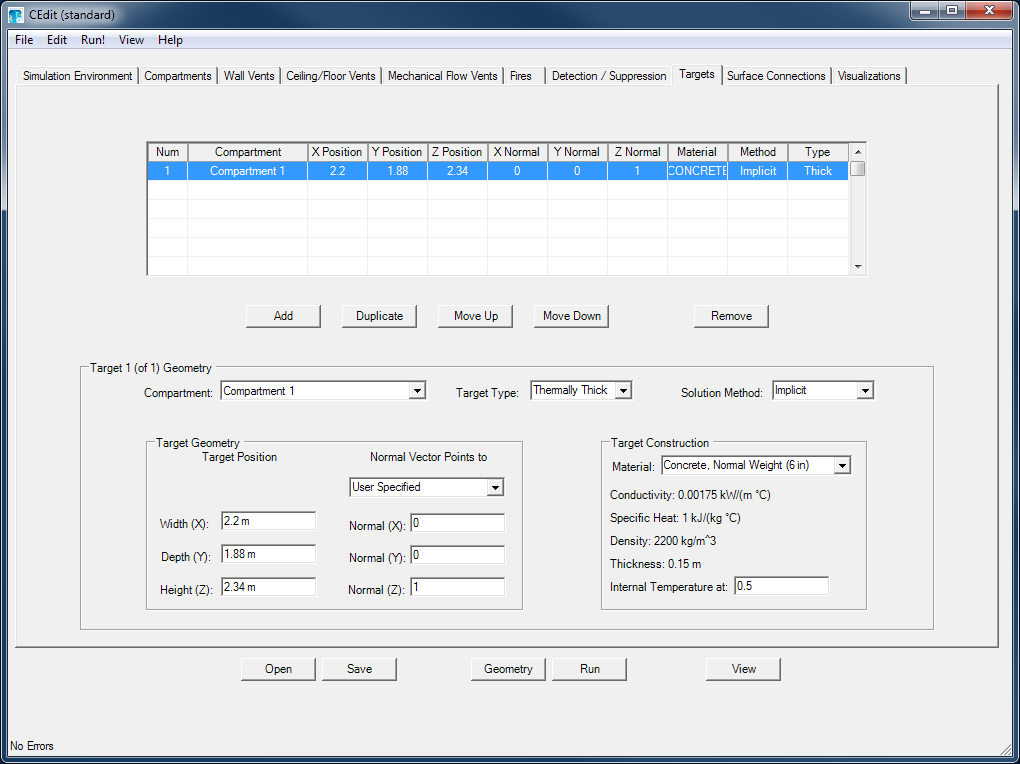
\includegraphics[width=6.5in]{FIGURES/Input_File/Target_Tab}
\end{center}
\end{figure}

In addition to any user-defined targets, there are always two targets that are automatically placed in any compartment containing a fire. Both are included for reporting purposes. The first is an “ambient target” and is intended to represent the net flux to a human body. This is used for the flux in the hazard calculation for tenability. The assumption is that the target will remain at ambient temperature, which is a surrogate for body temperature. The second determines the net flux to a horizontal target on the floor whose temperature is assumed to be the same as the floor surface. The calculation can be used to estimate the ignition of combustibles on the floor as a surrogate for estimating time to flashover, typically taken to be 20 kW/m$^2$. Thus if user-specified targets are included, they will be in addition to these two predefined targets.

For all targets, heat flux is calculated to the surface specified by the user (with the direction determined by the normal vector). Conduction into the target is assumed to occur only from this surface into the target.

\begin{description}
\item[Compartment] The compartment in which the target is located.

\item[Target Type] If the solution method is not STEADY, this parameter further indicates the solutions equations.  Specify Thermally Thick, Thermally Thin, or Cylindrical.  For thermally thin materials, CFAST uses ordinary differential equations; for thermally thick materials, partial differential equations, and for cylindrical targets, cylindrical coordinates.

\item[Solution Method] Optional parameter that indicates the solution method. STEADY for steady state solution, EXPLICIT for explicit solution, IMPLICIT for implicit solution.

\item[Width (X)] Position (default units: m, default value: none): Position of the target as a distance from the left wall of the target compartment (X direction).

\item[Depth (Y)] Position(default units: m, default value: none): Position of the target as a distance from the front wall of the target compartment (Y direction).

\item[Height (Z)] Position(default units: m, default value: none): Height of the target above the floor (Z direction).

\item[Normal Vector X] Component: specifies a vector of unit length perpendicular to the exposed surface of the target. (Width) component in the direction from the left wall of the target compartment. A value of 1 defines a vertical target facing into the compartment, unit vector = (1,0,0). The X, Y, and Z component of the normal vector can also be calculated automatically with a pull down menu that allows selection of surfaces and fires in the compartment visible from the target location.

\item[Normal Vector Y] Component: specifies a vector of unit length perpendicular to the exposed surface of the target. (Depth) component in the direction from the front wall of the target compartment. A value of 1 defines a vertical target facing to the right, unit vector = (0,1,0).

\item[Normal Vector Z] Component: specifies a vector of unit length perpendicular to the exposed surface of the target. (Height) component in the direction from the floor of the target compartment. Default value is a horizontal, upward facing target, unit vector = (0,0,1).

\item[Material] Used to specify the wall material of the target.  Any existing material in the list of thermal properties may be used here.

\item[Internal Temperature at] (default units: none, default value: 0.5): For each target, CFAST calculates the internal temperature at a number of node points within the target. By default, the reported internal temperature (in the printed and spreadsheet output) is the temperature at the center of the target, e.g., equidistant from the front and back faces of the target. This input allows the user to override this default position. The input represents the position as a fraction of the thickness from the front surface to the back surface of the material.
\end{description}

\graybox{
Target inputs in CFAST perform a heat transfer calculation between the compartment and the target. The steady state option assumes that the target material reacts instantly to changing conditions and computes the target temperature that would result in a balance of incoming and outgoing heat (i.e., a steady state). If a transient target temperature is modeled, then one can either assume that there is a temperature variation within the target or assume that the target is “thin” and can be modeled using only one temperature. If the target is assumed to be thin then the ODE option should be used set since this is how the equations are solved. If the target is assumed to be thick then the PDE option should set. Finally, if one of the two transient options are set (ODE or PDE), the numerical solution can be solved using an explicit or an implicit method.  Typically, the implicit method will work in all cases.  The explicit method is recommended only when the implicit method fails to come to a solution.
}



\chapter{Surface Connections}

\begin{figure}[h!]
\begin{center}
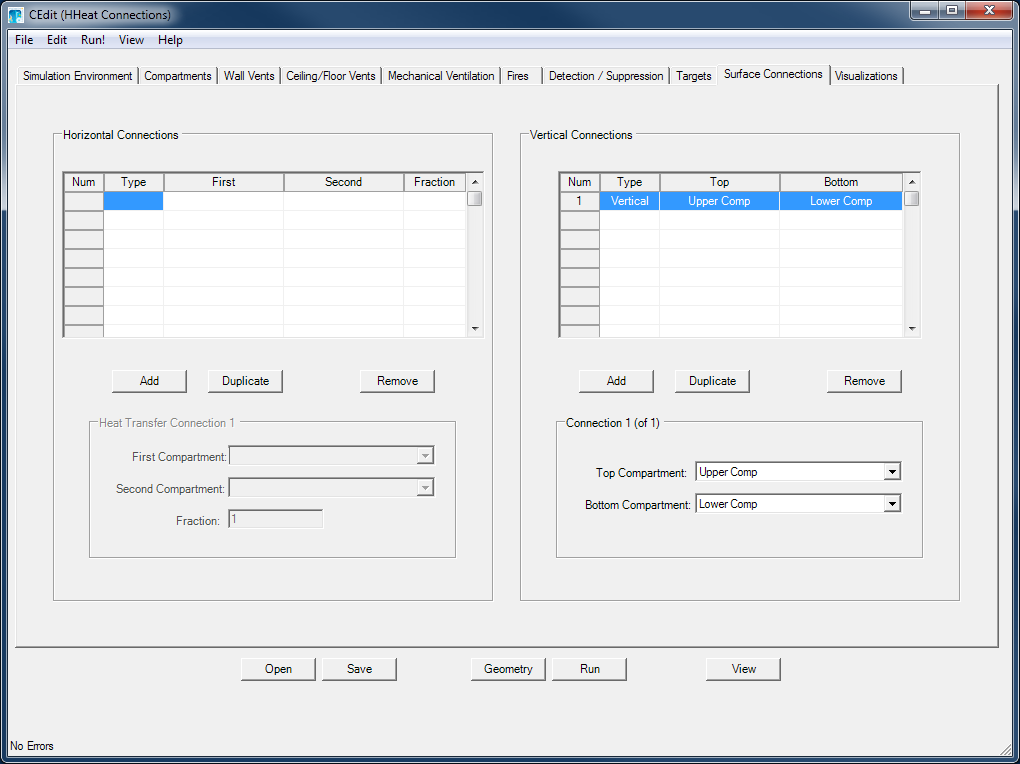
\includegraphics[width=6.5in]{FIGURES/Input_File/Surface_Connection_Tab}
\end{center}
\end{figure}

The Surface Connections page allows the user to define heat transfer between compartments in a simulation. Energy can be transferred from compartment to compartment through solid boundaries (walls, ceilings and floors) by means of conduction. The heat transfer between connected compartments is modeled by merging the connected surfaces for the ceiling and floor compartments or for the connected horizontal compartments.  The heat conduction problem is solved for the merged walls using a temperature boundary condition for both the near and far wall. As before, temperatures are determined by the solver so that the heat flux striking the wall surface (both interior and exterior) is consistent with the temperature gradient at that surface.

\begin{description}
\item[First Compartment] First of the connected compartments. Order of the inputs is not important.

\item[Second Compartment] Second of the connected compartments. Order of the inputs is not important.

\item[Fraction] Specifies the fraction of the vertical surface areas of the compartments which are connected can be specified. The fraction specifies the fraction of the vertical surface area connecting the first and second compartment pair.

\item[Top Compartment] The top or first of the two compartments to be connected by a vertical heat transfer connection. The connection is through the floor of this compartment.

\item[Bottom Compartment] The bottom or second of the two compartments to be connected by a vertical heat transfer connection. The connection is through the ceiling of this compartment.
\end{description}



\chapter{Visualization}

Calculated results from a CFAST simulation can be visualized using Smokeview \cite{Smokeview_Users_Guide_6}. This allows the user to see the compartment geometry and connections or view the results of the simulation visually. In addition to a simplified view of the layer temperatures and vent flows, more detailed estimates of gas temperature, gas velocity, vent flow velocity, target temperature, and detector status can be visualized.

\begin{figure}[h!]
\begin{center}
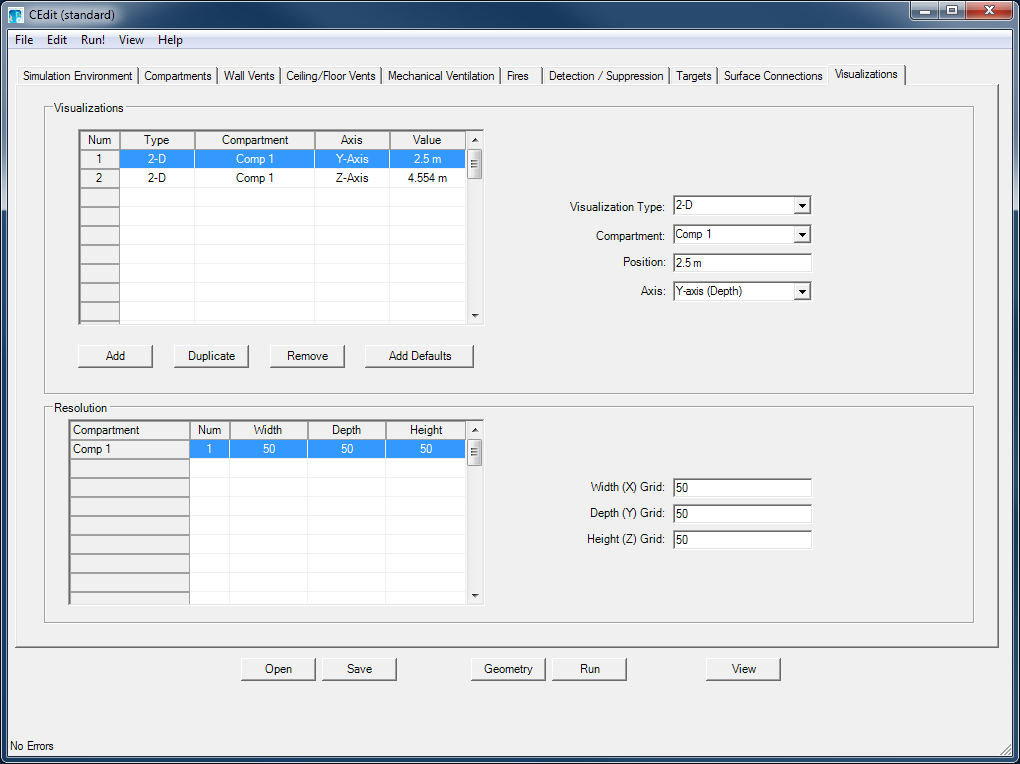
\includegraphics[width=6.5in]{FIGURES/Input_File/Visualizations_Tab}
\end{center}
\end{figure}

\section{Adding Visualizations}

\begin{description}
\item[Visualization Type] (default units: n/a, default value: 2-D): The type of visualization to be included. Choose from 2-D (a single plane slice of temperature at the position and axis specified), 3-D (a set of three animated slices whose position can be moved along its respective axis, or Isosurface (a fixed 3-D surface where the gas temperature is equal to the value specified. See the Smokeview documentation \cite{Smokeview_Users_Guide_6}for details on the use of Smokeview.

\item[Compartment] (default units: n/a, default value: All): Visualizations can be placed in a single compartment or at the same position and axis in all compartments.

\item[Position] (default units: m, default value: 0m): Position along the specified axes where the slice is placed measured from the compartment origin for the selected axis (0,0,0 is the bottom left corner of the compartment. See page \pageref{Compartment_Geometry}).

\item[Axis] (default units: n/s, default value: X-axis (Width)): Axis that the specified slice file is located.  The slice is place perpendicular to the selected axis (the Y-Z plane for the X-Axis; the X-Z plane for the Y-Axis, and the X-Y plane for the Z-Axis)

\item[Temperature] (default units \degc, default value: none): Specified gas temperature for the selected isosurface.
\end{description}

\graybox{
Use the Add Defaults button to add a default set of visualizations for the current simulation. A slice file entry is created at the center of each compartment in the x (width) and y (depth) directions along with one near the ceiling in the z direction. a 3-D slice file entry is created for each compartment as well.
}

\section{Visualization Resolution}

By default, slice files are generated with a grid of 50 data points in each direction for each compartment specified. If desired, the grid spacing can be adjusted up or down individually by compartment. Specifying a larger number of data points can \textit{dramatically} slow program execution since the gas temperature and velocity is evaluated at each grid location every time a Smokeview output is specified.  The default value should be appropriate for most simulations.

\begin{description}
\item[Width (X) Grid] (default units: n/a, default value: 50): slices included along the X axis for each compartment are uniformly divided into the specified number of data points.

\item[Width (Y) Grid] (default units: n/a, default value: 50): slices included along the Y axis for each compartment are uniformly divided into the specified number of data points.

\item[Width (Z) Grid] (default units: n/a, default value: 50): slices included along the Z axis for each compartment are divided into the specified number of data points.
\end{description}

Sample visualizations are included below.

\begin{figure}[h!]
\begin{center}
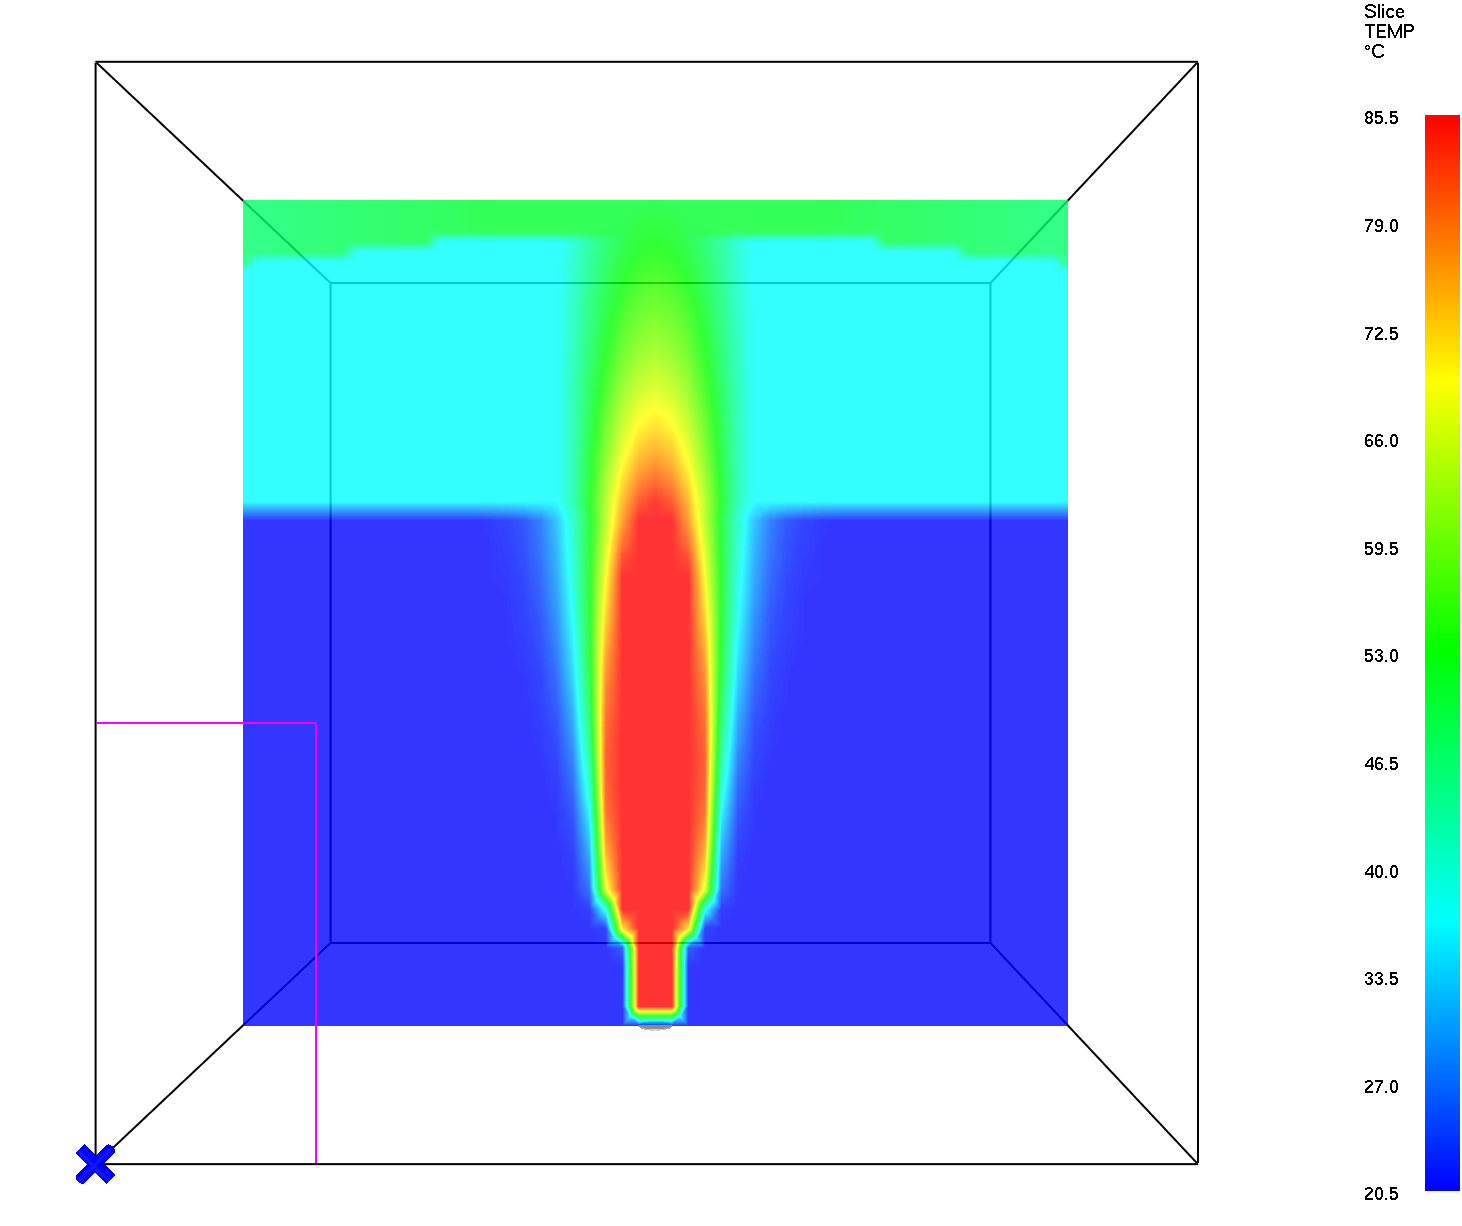
\includegraphics[width=6.5in]{FIGURES/Input_File/SMV_Temperature}
Smokeview Visualization of Gas Temperature with a Single Fire
\end{center}
\end{figure}

\begin{figure}[h!]
\begin{center}
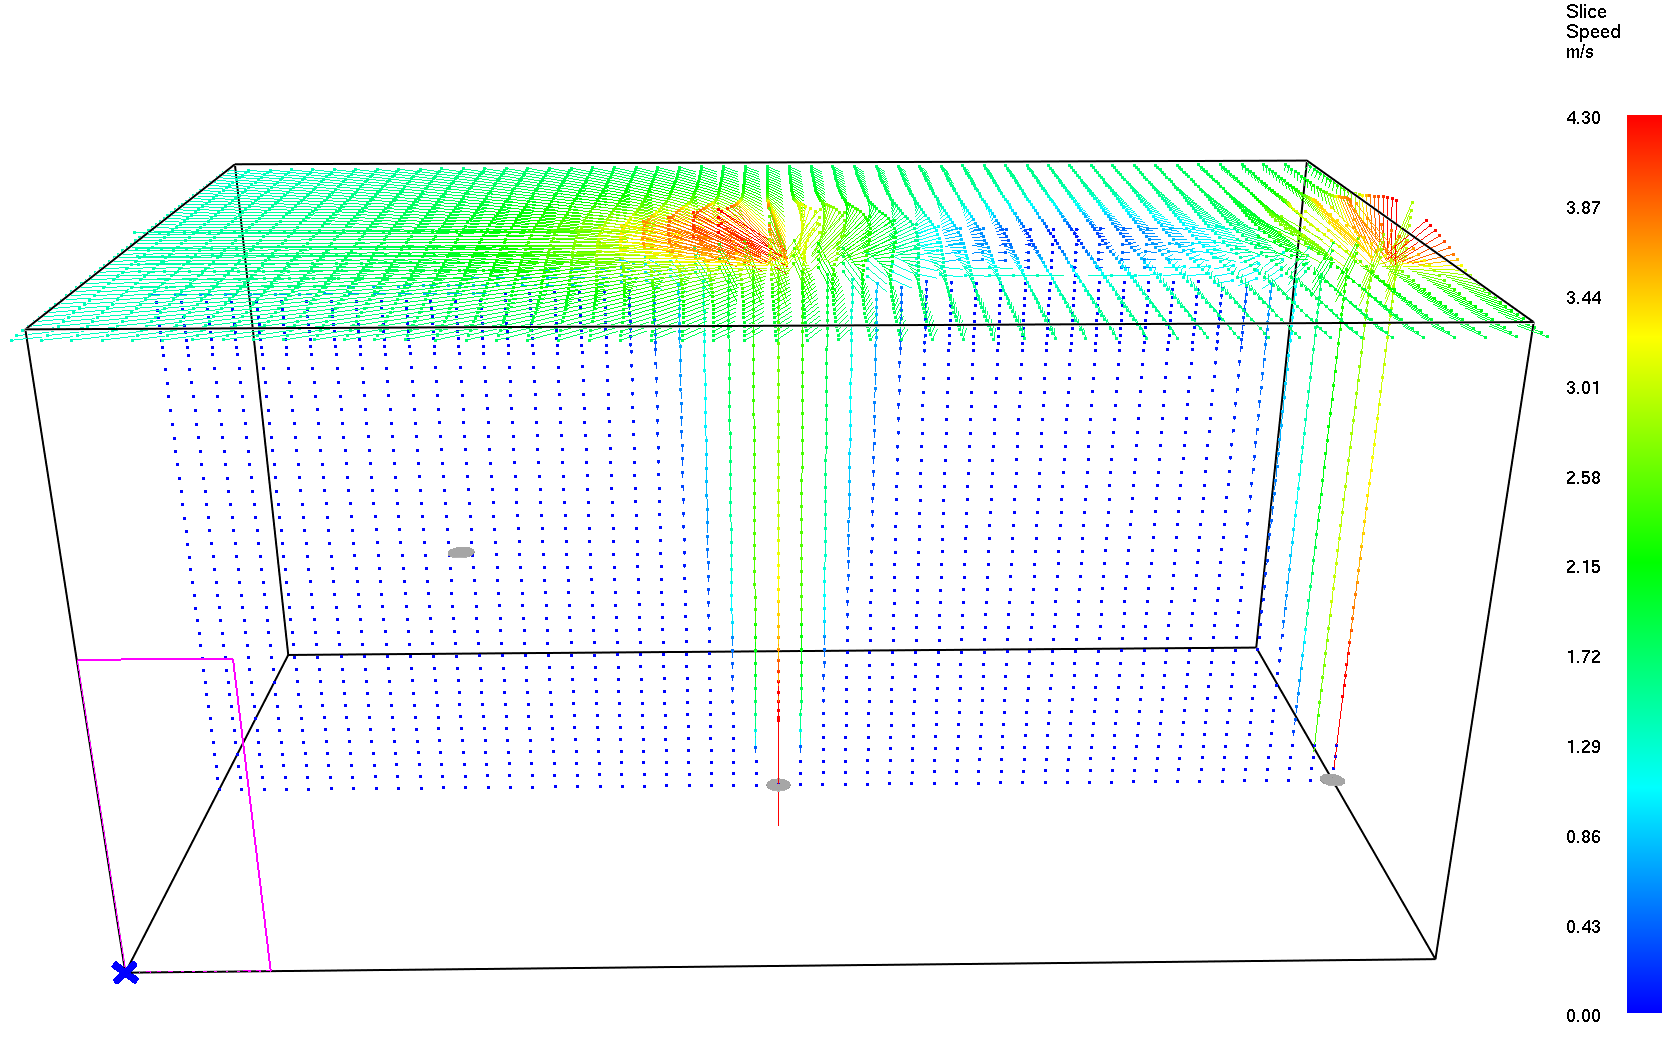
\includegraphics[width=6.5in]{FIGURES/Input_File/SMV_Velocity}
Smokeview Visualization of Gas Velocity with Two Fires
\end{center}
\end{figure}

\begin{figure}[h!]
\begin{center}
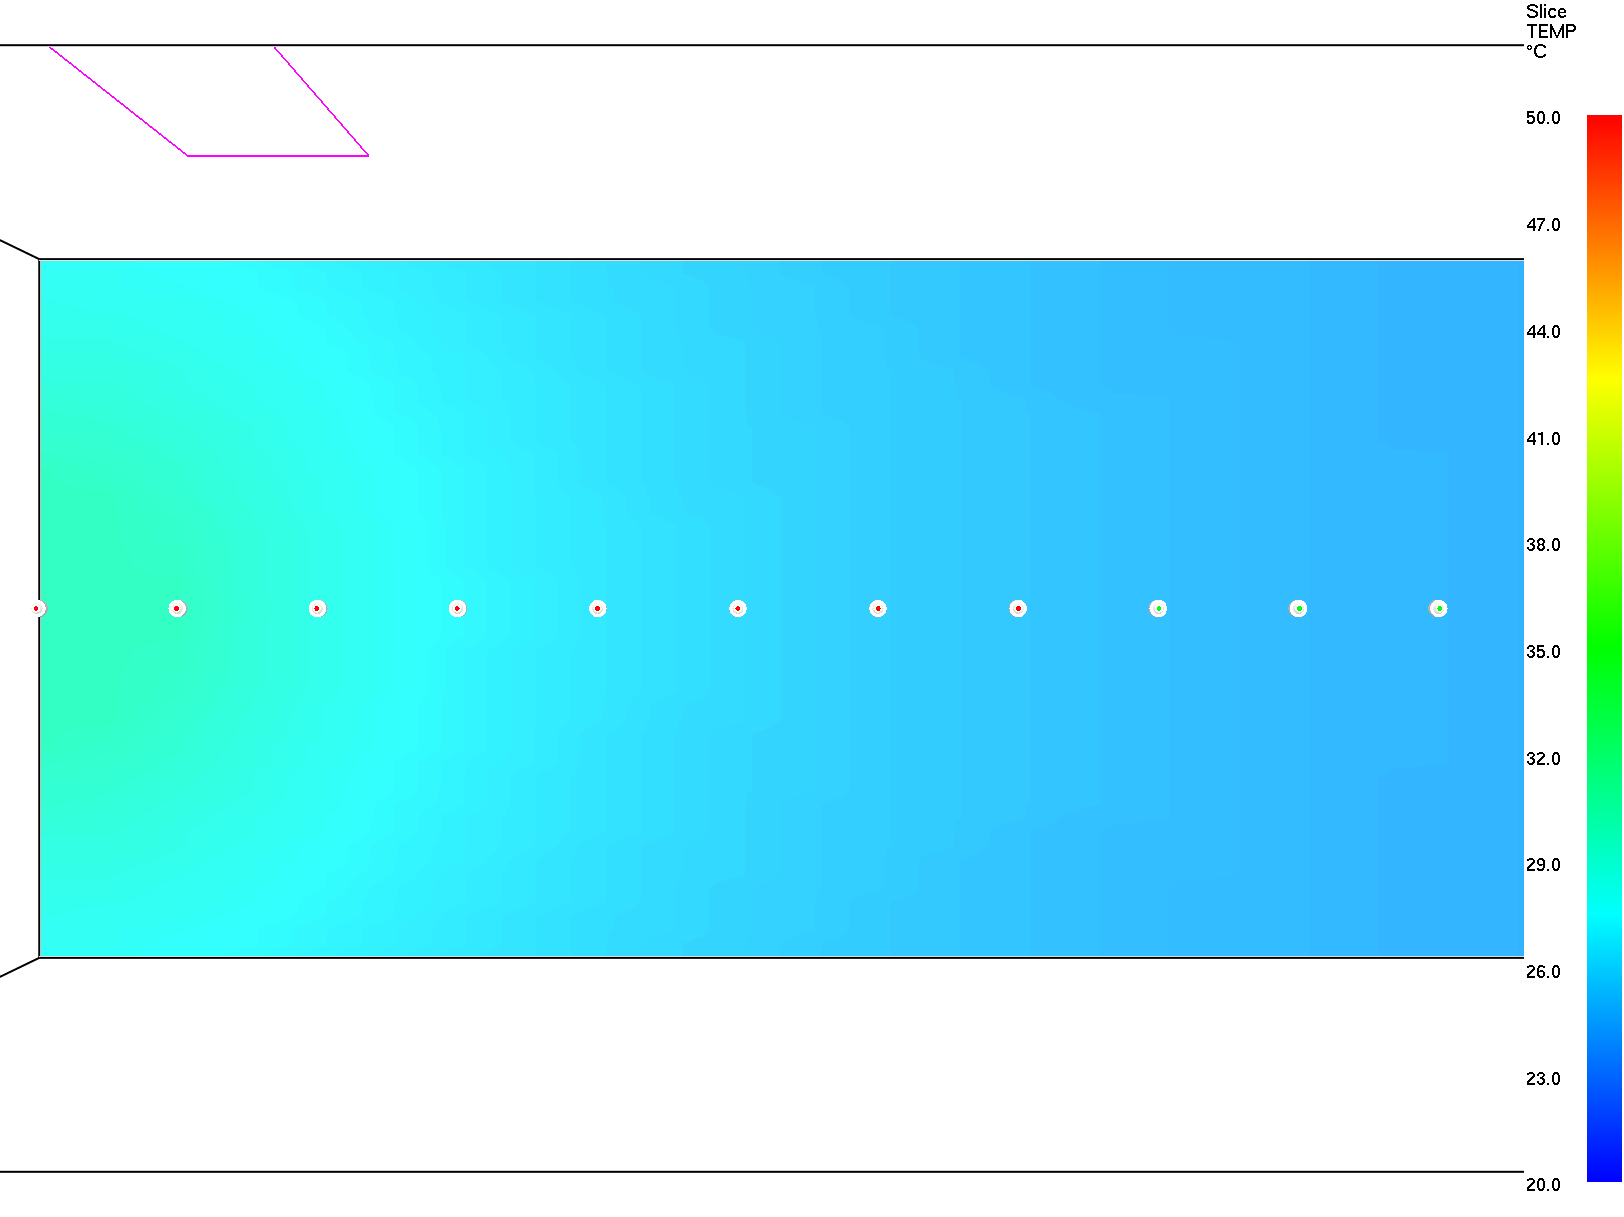
\includegraphics[width=6.5in]{FIGURES/Input_File/SMV_Detectors}
Smokeview Visualization of Detector Activation in a Corridor
\end{center}
\end{figure}


\chapter{Output from CFAST}
\label{Output_Chapter}

The output of CFAST includes the temperatures of the upper and lower gas layers within each compartment, the ceiling/wall/floor temperatures within each compartment, the visible smoke and gas species concentrations within each layer, target temperatures and sprinkler activation time.  The amount of information can be very large, especially for complex geometries and long simulations.

\section{Compact Output}

The default output to the console is called the compact form, and shows the basic information about a scenario, including layer temperatures and the size of fires. Default text output provides a simple overview for the user to make sure the case runs as expected.
\begin{lstlisting}[basicstyle=\scriptsize]
 Time =   1800.0 seconds.

 Compartment   Upper   Lower   Inter.  Pyrol     Fire      Pressure  Ambient
               Temp.   Temp.   Height  Rate      Size                Target
               (C)     (C)     (m)     (kg/s)    (W)       (Pa)      (W/m^2)
 -----------------------------------------------------------------------------
    1          113.4    33.3    1.4     1.393E-02 3.000E+05-0.790      523.
  Outside                                         0.00
\end{lstlisting}
The first column contains the compartment number.  On each row with its compartment number from left to right is the upper layer temperature, lower layer temperature, the height of the interface between the two layers, the total pyrolysis rate, and finally the total fire size.  The only value given for the outside is the total heat release rate of fires venting to the outside.

\section{Detailed Outputs}

The following sections describe each of the outputs from the model.  Each section refers to a specific part of the print out and appears in the order the output appears. A description of each option follows.

\subsection{Output for Initialization}

This option prints the initial conditions to the output before the actual run starts.  This merely mimics the inputs specified by the user in the input data file  The initial conditions break down into seven sections.  Each is described below with the section name. The following explanation uses the output from the case STANDARD.IN. STANDARD.IN is included in the distribution. Please note, there are no mechanical ventilation, horizontal vents or detectors in this example, so the section discussing these phenomena are from additional data files.

\subsubsection{Overview}

The overview gives a general description of the case.  The output is fairly self explanatory. ``Doors, ...'' is the total number of horizontal natural flow vent connections in all compartments of the simulation.  ``Ceil. Vents, ...'' gives the total number of vertical natural flow vent connections in all compartments of the simulation.  The last header on the line ``MV Connections'' has the total number mechanical flow connections to all compartments in the simulation. Times in these outputs come from the TIMES input. All times are in s.
\begin{lstlisting}[basicstyle=\scriptsize]
 OVERVIEW


Compartments    Doors, ...    Ceil. Vents, ...    MV Connects
   1               1             0                    0

Simulation     Output         Smokeview      Spreadsheet
Time           Interval       Interval       Interval
(s)            (s)            (s)            (s)
  1800         120             10             30
\end{lstlisting}

\subsubsection{Ambient Conditions}

This section, like the overview section, needs little elaboration.  It gives the starting atmospheric conditions for the simulation both for outside and inside the structure. Data for these outputs come from the TAMB and EAMB inputs. Temperatures are in K, pressure in Pa, elevations in m, and wind speed in m/s. Wind Power is the dimensionless power law coefficient from the WIND input.
\begin{lstlisting}[basicstyle=\scriptsize]
 AMBIENT CONDITIONS

 Interior       Interior       Exterior       Exterior
 Temperature    Pressure       Temperature    Pressure
   (C)            (Pa)           (C)            (Pa)

     20.          101300.          20.          101300)
\end{lstlisting}

\subsubsection{Compartments}

The compartments section gives a summary of the geometry for the simulation.  A simple table summarizes the geometry with compartments running down the page in numerical order.  The various dimensions for each compartment are on the row with its compartment number.  Two columns need explanation.  The second to last column ``Ceiling Height'' gives the height of the ceiling relative to the station height in the Ambient Conditions section.  Similarly the ``Floor Height'' refers to the height of the floor above the station height.

\begin{lstlisting}[basicstyle=\scriptsize]
COMPARTMENTS

Compartment  Name                Width        Depth        Height       Ceiling      Floor
                                                                        Height       Height
                                 (m)          (m)          (m)          (m)          (m)
------------------------------------------------------------------------------------------------
    1        Compartment 1        9.10         5.00         4.60         4.60         0.00
\end{lstlisting}


\subsubsection{Horizontal Natural Ventilation}

This is the first table in the vent connections section.  Each row in the table characterizes one vent.  The first two columns contain the two compartments connected by the vent.  Each vent is ordered first by the lower number of the two compartments and then the numeric order of the second compartment.  The third column gives the vent number.  Column four is the width of the vent.  The next two columns report the sill and soffit height for the vent relative to the floor of the first compartment.  The seventh and eighth columns have a second listing of the sill and soffit height, this time relative to the station height.

\begin{lstlisting}[basicstyle=\scriptsize]
VENT CONNECTIONS

Horizontal Natural Flow Connections (Doors, Windows, ...)

From           To             Vent       Width       Sill        Soffit      Abs.        Abs.
Compartment    Compartment    Number                 Height      Height      Sill        Soffit
                                         (m)         (m)         (m)         (m)         (m)
----------------------------------------------------------------------------------------------------
Compartment 1   Outside        1          1.00        0.00        2.40        0.00        2.40
\end{lstlisting}
From compartment, to compartment, vent number, width, sill height, and soffit height all come directly from the HVENT specifications in the input data file. Absolute sill height is the station elevation + compartment floor height + sill height. Absolute soffit height is the station elevation + compartment floor height + soffit height.

\subsubsection{Vertical Natural Ventilation}

The first column is the upper compartment.  The upper compartment is the compartment where the vent opens into the floor.  The second column is the lower compartment where the vent is in the ceiling.  The third column describes the shape of the vent, which can be either round or square.  The fourth column gives the area of the vent.  The last two columns are the height of the vent, relative to the floor of the lower room and relative to the station height respectively.
\begin{lstlisting}[basicstyle=\scriptsize]
Vertical Natural Flow Connections (Ceiling, ...)

Top            Bottom         Shape     Area      Relative  Absolute
Compartment    Compartment                        Height    Height
                                        (m^2)     (m)       (m)
----------------------------------------------------------------------
 Outside           1          Round      1.00      4.60      4.60
\end{lstlisting}
Top compartment, bottom compartment, shape, and area come from the VVENT specifications in the input data file. Relative height is the height of the vent above the floor of the bottom compartment and absolute height is the height of the vent above the station elevation.

\subsubsection{Mechanical Flow Connections}

This section lists all connections to compartments and fans that connect between compartments. The table lists, in order, the number of the system the fan is a part, the ``from'' node and its height, the ``to'' node and its height.  A fan actually draws air from the first or ``from'' node and pushes it to the second or ``to'' node. The sixth column is the cross-sectional area of the duct connection to the chosen compartment. The seventh column is the fan number as defined in CEdit.  The next two columns are the minimum and maximum pressures at which the fan curve is defined.  The rest of the row is made up of the one to five fan curve coefficients in the input file.

\begin{lstlisting}[basicstyle=\tiny]
FANS

System    From           From      To             To        Area      Fan       Minimum   Maximum    Flowrate
                         Elev.                    Elev.               Number
                         (m)                      (m)       (m^2)               (Pa)      (Pa)       (m^3/s)
--------------------------------------------------------------------------------------------------------------
   1      Comp  1        1.00      Node  1        1.00      0.05
          Node  1        1.00      Node  2       10.00                  1       200.00    300.00     3.80E-02
          Node  2       10.00      Outside       10.00      0.05
\end{lstlisting}

\subsubsection{Thermal Properties}

The thermal properties section is broken into two parts.  The first part is a table that lists the material for each surface of each compartment.  The compartments appear as rows down the page in numerical order.  From left to right next to the compartment number comes the material for the ceiling, wall and floor.  The second part lists the properties of each material used in the simulation. For each listing of a material, the name is followed by the conductivity, specific heat, density, thickness and emissivity. In addition to materials for compartment surfaces, any thermal properties specified for targets are also listed (this may include thermal properties for gaseous materials specified as fire sources in a simulation.

\begin{lstlisting}[basicstyle=\scriptsize]
 THERMAL PROPERTIES

 Compartment    Ceiling      Wall         Floor
 ----------------------------------------------------
 Compartment 1  GLASSFB3     CONCRETE     CONCRETE

 Name    Conductivity Specific heat     Density     Thickness   Emissivity
 CONCRETE     1.75        1.000E+03    2.200E+03    0.150        0.940
 GLASSFB3    3.600E-02     795.         105.        1.300E-02    0.900
 HARDWOOD    0.160        1.255E+03     720.        1.900E-02    0.900
 DEFAULT     0.120         900.         800.        1.200E-02    0.900
\end{lstlisting}
Material choices of the ceiling, walls, and floors come from the CEILI, WALLS, and FLOOR specifications in the input data file. Units for thermal properties are standard S.I. units.  For thermal conductivity, W/m K; for specific heat, J/kg K; for density, kg/m$^3$; for thickness, m; emissivity is dimensionless.


\subsubsection{Targets}

The entry for targets shows the orientation of additional targets specified in the data file. Targets explicitly specified in the data file are listed first in the order they are included in the data file.  Each target is numbered based on the order of the target specifications in the input data file.  The compartment number, position of the target within the compartment, direction of the front face of the target object expressed as a normal unit vector to the surface, and object material. Additional targets, one for each compartment and one for each fire are automatically generated by the program and included in the list after the user-specified targets.

\begin{lstlisting}[basicstyle=\scriptsize]
TARGETS

Target  Compartment    Position (x, y, z)         Direction (x, y, z)      Material
----------------------------------------------------------------------------------
    1     Comp 1       2.20     1.88     2.34     0.00     0.00     1.00   CONCRETE
    2     Comp 1       4.55     2.50     0.00     0.00     0.00     1.00   METHANE
    3     Comp 1       4.55     2.50     0.00     0.00     0.00     1.00   HARDWOOD
    4     Comp 1       4.55     2.50     0.00     0.00     0.00     1.00   CONCRETE
\end{lstlisting}
All of the inputs for targets come from the TARGE command in the input data file. Direction is specified as a unit vector as described in the section on target input. Units for position and direction are all in m.


\subsubsection{Fires}

The fire section lists all the information about the main fire and any object fires that might exist.  All the information for each fire is listed separately.  If there is a main fire, it comes first.  Each fire listing has the same form.  First is the name of the fire followed by a list of general information.  Listed left to right is the compartment the fire is in, the type of fire, the x, y, z position, the relative humidity, the lower oxygen limit, and finally the radiative fraction for the fire.

A table of time history curves for the fire follows.  The table contains all the time history curves for the fire.  Each row on the table is a specific time given in the left most column.  The rest of the columns give the values at that particular time.  The column headers indicate each input quantity and correspond to specific keywords in the fire definition. The headings are defined as follows: `Fmdot' is pyrolysis rate; `Hcomb' is the heat of combustion; `Fqdot' is the heat release rate; `Fheight' is height of fire; `Soot' is the fraction of the fuel mass converted to soot during combustion; `CO' is the fraction of the fuel mass converted to carbon monoxide during combustion; `HCN' is the fraction of the fuel mass converted to hydrogen cyanide during combustion; `HCl' is the fraction of the fuel mass converted to hydrogen chloride during combustion; `CT' is the concentration-time product; and `TS' is the fraction of fuel mass converted to trace species during combustion.

\begin{lstlisting}[basicstyle=\tiny]
FIRES

Name: bunsen   Referenced as object #  1

Compartment    Fire Type       Position (x,y,z)     Relative    Lower O2    Radiative
                                                    Humidity    Limit       Fraction
Compartment 1  Constrained     4.55   2.50   0.00   50.0        10.00        0.33


Chemical formula of the fuel
  Carbon    Hydrogen  Oxygen    Nitrogen  Chlorine
  1.000     4.000     0.000     0.000     0.000


  Time      Fmdot     Hcomb     Fqdot     Fheight   Soot      CO        HCN       HCl       CT        TS
  (s)       (kg/s)    (J/kg)    (W)       (m)       (kg/kg)   (kg/kg)   (kg/kg)   (kg/kg)   (kg/kg)   (kg/kg)
----------------------------------------------------------------------------------------------------------------
     0.      0.0      5.00E+07   0.0       0.0       0.0      1.05E-03   0.0       0.0       1.0       0.0
    60.     2.00E-03  5.00E+07  1.00E+05   0.0       0.0      1.05E-03   0.0       0.0       1.0       0.0
   120.     3.00E-03  5.00E+07  1.50E+05   0.0       0.0      1.05E-03   0.0       0.0       1.0       0.0
   180.     4.00E-03  5.00E+07  2.00E+05   0.0       0.0      1.05E-03   0.0       0.0       1.0       0.0
   240.     3.00E-03  5.00E+07  1.50E+05   0.0       0.0      1.05E-03   0.0       0.0       1.0       0.0
   300.     2.50E-03  5.00E+07  1.25E+05   0.0       0.0      1.05E-03   0.0       0.0       1.0       0.0
   360.     2.00E-03  5.00E+07  1.00E+05   0.0       0.0      1.05E-03   0.0       0.0       1.0       0.0
   420.     1.80E-03  5.00E+07  9.00E+04   0.0       0.0      1.05E-03   0.0       0.0       1.0       0.0
   480.     1.60E-03  5.00E+07  8.00E+04   0.0       0.0      1.05E-03   0.0       0.0       1.0       0.0
   540.     1.50E-03  5.00E+07  7.50E+04   0.0       0.0      1.05E-03   0.0       0.0       1.0       0.0
  1800.     1.50E-03  5.00E+07  7.50E+04   0.0       0.0      1.05E-03   0.0       0.0       1.0       0.0


Name: Wood_Wall   Referenced as object #  2

Compartment    Fire Type       Position (x,y,z)     Relative    Lower O2    Radiative
                                                    Humidity    Limit       Fraction
Compartment 1  Constrained     4.55   2.50   0.00   50.0        10.00        0.33


Chemical formula of the fuel
  Carbon    Hydrogen  Oxygen    Nitrogen  Chlorine
  6.000    10.000     5.000     0.000     0.000


  Time      Fmdot     Hcomb     Fqdot     Fheight   Soot      CO        HCN       HCl       CT        TS
  (s)       (kg/s)    (J/kg)    (W)       (m)       (kg/kg)   (kg/kg)   (kg/kg)   (kg/kg)   (kg/kg)   (kg/kg)
----------------------------------------------------------------------------------------------------------------
     0.      0.0      1.81E+07   0.0       0.0      2.00E-02  2.00E-02   0.0       0.0       1.0       0.0
  8000.     5.52E-02  1.81E+07  1.00E+06   3.0      2.00E-02  2.00E-02   0.0       0.0       1.0       0.0
\end{lstlisting}
All of the inputs for the main fire come from the fire specifications in the input data file. Data for the object fire comes from the object data file included with the CFAST software. Units for most values are included in the output.  Fire position is in m, relative humidity is in \%, lower oxygen limit is in volume percent, and pyrolysis temperature is in K.


\subsection{Output for Main Variables}

The normal print out is the first information printed at each time interval.  This information includes the layer temperatures, interface height, volume of the upper layer, layer absorption coefficients, and compartment pressure (relative to ambient).

\begin{lstlisting}[basicstyle=\scriptsize]
 Time =   1800.0 seconds.

 Compartment   Upper     Lower     Inter.    Upper           Upper      Lower     Pressure
               Temp.     Temp.     Height    Vol.            Absorb     Absorb
                (C)      (C)       (m)       (m^3)           (m^-1)     (m^-1)      (Pa)
 ------------------------------------------------------------------------------------------
 Comp 1         113.4    33.30     1.410     1.45E+02( 69%)  0.124      8.817E-02  -0.790
\end{lstlisting}
The second table of the normal print out has information about the fires.  In essence it is two tables joined.  The first part lists information by fire.  It starts with the main fire, if there is one, and then the object fires down the page.  The fires are listed in the second column followed by the plume flow rate, the pyrolysis rate, the fire size, and flame height.  The next three columns are then skipped.  The next column with information is the amount of heat given off by each fire convectively, followed by the amount of heat given off radiantly. The last two columns give the total mass pyrolyzed and the amount of trace species produced.  The second part starts after all the fires have been individually listed.  It gives the totals for all fires in each compartment.  The first column has the compartment number.  The compartments start at one and are listed down the page in order.  The third to fifth columns are the same as the first part except the values are totals for the compartment and not just for one fire.  The sixth column has the total heat release rate that occurs in the upper layer.  The next column has the same total in the lower layer.  The eighth column has the total size of vent fires in the compartment.

\begin{lstlisting}[basicstyle=\tiny]
FIRES

Compartment    Fire      Plume   Pyrol     Fire      Flame   Fire in   Fire in   Vent    Convec.   Radiat.    Pyrolysate  Trace
                         Flow    Rate      Size      Height  Upper     Lower     Fire
                         (kg/s)  (kg/s)    (W)       (m)     (W)       (W)       (W)     (W)       (W)        (kg)        (kg)
 -------------------------------------------------------------------------------------------------------------------------------
                bunsen   0.356   1.500E-03 7.500E+04 0.958                               5.025E+04 2.475E+04  3.13        0.00
              Wood_Wal   0.921   1.243E-02 2.250E+05 0.397                               1.507E+05 7.425E+04  11.2        0.00

Comp 1                    1.28   1.393E-02 3.000E+05          0.00     3.000E+05  0.00
\end{lstlisting}
Flame height is calculated from the work of Heskestad~\cite{Heskestad:2002}. The average flame height is defined as the distance from the fuel source to the top of the visible flame where the intermittency is 0.5.  A flame intermittency of 0.5 means that the visible flame is above the mean 50~\% of the time and below the mean 50~\% of the time.


\subsection{Output for Wall Surfaces, Targets, and Detectors/Sprinklers}

The printed output provides two tables displaying information about wall surface or target temperatures and fluxes, and heat detectors or sprinklers. The left most column specifies the compartment number; followed by four columns providing the temperatures of the bounding surfaces of the compartment in contact with the ceiling, upper wall surface (in contact with the upper layer gases), lower wall surface (in contact with the lower layer gases), and floor, in that order. Next comes information about targets in the compartment, with each target listed on a separate line.  Information in the columns includes the surface temperature of the target, net heat flux to the target, and the percentage of that net flux that is due to radiation from the fire, radiation from compartment surfaces, radiation from the gas layers, and convection from the gas surrounding the target.  CFAST includes one target in the center of the floor for all compartments. Information on additional targets specified by the user in the input data file are also included, in the order specified in the input file.

For smoke detectors, heat detectors, and sprinklers, the temperature of the device, its current state (activated or not), and the nearby gas temperature and velocity are included.

\begin{lstlisting}[basicstyle=\tiny]
SURFACES AND TARGETS


Compartment  Ceiling Up wall Low wall Floor Target Gas   Surface Center Flux To Fire      Surface Gas
             Temp.   Temp.   Temp.    Temp.        Temp. Temp.   Temp.  Target  Rad.      Rad.    Rad.    Convect.
             (C)     (C)     (C)      (C)          (C)   (C)     (C)    (W/m^2) (W/m^2)   (W/m^2) (W/m^2) (W/m^2)
------------------------------------------------------------------------------------------------------------------
Comp 1       23.0    22.5    21.6     22.6  Floor       22.6            17.8   2.817E-02  13.3    1.25    3.23
                                            1     23.7  21.7    20.9    23.2   0.00       12.0    1.54    9.67
                                            2     21.2  21.7    21.7    16.6   1.341E-04  12.0    1.46    3.23
                                            3     21.2  25.0    25.0    16.6   1.341E-04  12.0    1.46    3.23
\end{lstlisting}

\begin{lstlisting}[basicstyle=\scriptsize]
DETECTORS/ALARMS/SPRINKLERS

                             Sensor                           Smoke
Number  Compartment   Type   Temp (C)   Activated       Temp (C)   Vel (m/s)
----------------------------------------------------------------------------
 1        1           HEAT   2.627E+01  YES             2.518E+01  6.617E-01
\end{lstlisting}
In all cases, the flux to/from a target is net radiation or net convection. That is, it is the incoming minus the outgoing. So while a target or object is heating, the flux will be positive, and once it starts to cool, the flux will be negative. Values for radiation from fires (fire rad.), radiation from surfaces (surface rad.), radiation from the gas layers (gas rad.), and convection from surfaces (convect) are expressed as the net flux to target (flux to target). Positive values indicate heat gains by the target and negative values indicate heat losses.


\subsection{Output for Gas Species}

The output has two tables displaying information about the amounts of species in each layer. The species information follows the normal print out.  The first table gives species volume fractions for the upper layers of all the compartments and the second reports the same for the lower layers of all the compartments.  Again the compartments are listed down the page and the information across the page.  The species are each given in one of several different terms.  Below each header are the units for the given value.  Most of the headers are simply the chemical formula for the species being tracked.  However, several are not obvious.  ``TUHC'' is the total unburned hydrocarbons or the pyrolyzed fuel that hasn't burned yet.  ``OD'' is the optical density, which is a measure of the amount of smoke. ``TS'' is trace species.

\begin{lstlisting}[basicstyle=\scriptsize]
UPPER LAYER SPECIES

compartment   N2    O2     CO2       CO    HCN   HCL   TUHC H2O   OD        CT         TS
              (%)   (%)    (%)       (ppm) (ppm) (ppm) (%)  (%)   (1/m)     (g-min/m3) kg
----------------------------------------------------------------------------------------------
Compartment 1 79.2  20.5  9.055E-02  2.98  0.00  0.00  0.00 0.180 1.086E-02 51.8       0.00


LOWER LAYER SPECIES

compartment   N2    O2    CO2        CO     HCN   HCL   TUHC H2O   OD        CT         TS
              (%)   (%)   (%)        (ppm)  (ppm) (ppm) (%)  (%)   (1/m)     (g-min/m3) kg
----------------------------------------------------------------------------------------------
Compartment 1 79.3  20.7  6.412E-03  0.211  0.00  0.00  0.00 0.029 7.750E-04 4.00      0.00
\end{lstlisting}
The report by species for nitrogen, oxygen, hydrogen chloride and the total unburned hydrocarbons (fuel vapor in the layer) are percent by volume. Carbon dioxide, carbon monoxide and hydrogen cyanide are in parts per million, which is proportional to the volume fraction.  Optical depth per meter is a measure of the visibility in the smoke. This is covered in detail in the comment on visibility in the section on fires and species specification. The concentration-time (CT) calculation is an integration of the species input for type CT (See section \ref{sec:fire_inputs} for the input of CT) and is intended to represent a relative dose of toxic gas species. Trace species (TS) is the total kilograms of the trace species that is present in the compartment. It is an absolute measure and not percent or density.


\subsection{Output for Vent Flows}

Information about vent flow is obtained by using this option.  It includes a section detailing mass flow through horizontal, vertical, and mechanical vents. There are two forms for the vent flow. The first is flow through the vents as mass per second. The alternative, obtained with the total mass flow output option on the `Run!,' `Output Options' menu, gives the total mass which has flowed through the vent(s) and the relative mass of trace species divided by the total mass of trace species produced up to the current time.

The section for vent flow is titled ``FLOW THROUGH VENTS (kg/s).''  Because flow is always given in positive values, each vent is listed twice, once for flow going from compartment A to compartment B (labelled as ``Flow relative to `from''') and a second time for flow from B to A (labelled as ``Flow relative to `To'''.  As the example below shows, the first column specifies the vent, including the type of vent (an ``H'' in this column stands for horizontal flow, such as through a doorway or window; a ``V'' here would mean vertical flow, such as through an opening in the ceiling, and an ``M'' stands for a mechanical ventilation connection) and the compartment from which the flow comes. The second column lists the name of the compartment. Up to six additional columns detail the flow at this vent. Flow into and out of the compartment through the vent in the upper and lower layers are included.

\begin{lstlisting}[basicstyle=\tiny]
 FLOW THROUGH VENTS (kg/s)

                                        Flow relative to 'From'                Flow Relative to 'To'
                                        Upper Layer               Lower Layer  Upper Layer               Lower Layer
 Vent From/Bottom    To/Top     Inflow  Outflow      Inflow       Outflow      Inflow       Outflow      Inflow       Outflow
---------------------------------------------------------------------------------------------------------------------------------
 H  1 Comp1          Outside            1.000        0.974                     1.000                                  0.974
\end{lstlisting}
The mass balance is the sum of the flow in minus the flow out. (Note that this is an extended run to achieve results close to steady state.) For any compartment, this is just
$$
\brackets{\dm_{u,in} + \dm_{l,in} + \dm_f} - \brackets{\dm_{u,out} + \dm_{l,out}}
$$
with the inflow and outflow summed for each vent. For the above example, the mass balance is:
$$(0.974 + 0.01393)~\hbox{kg/s} - (1.000)~\hbox{kg/s} = -0.012~\hbox{kg/s}$$
where the pyrolysis rate (from the ``normal'' output) is 0.01393 kg/s. The result is about the right magnitude (about 1 \% of the mass flow into or out of the vent) for net mass loss given the default equation solver tolerances for CFAST.  The mass loss should still be slightly negative since the compartment continues to heat.

An alternative printout is provided by use of the total mass flow output option on the `Run!,' `Output Options' menu. This shows total (mass) flow through vents. At present this is confined to mechanical ventilation. It applies only to vents which can be filtered, in this case mechanical ventilation. The last column is obtained by summing the outflow/inflow for each vent and then dividing that sum by the total trace species produced by all fires. For details on this value, see the section on output listing for fires.

\begin{lstlisting}[basicstyle=\tiny]
Total mass flow through vents (kg)

To             Through              Upper Layer               Lower Layer           Trace Species
Compartment    Vent             Inflow       Outflow      Inflow       Outflow      Relative to Total Release
-------------------------------------------------------------------------------------------------------------
Comp 1         M Node  1                    63.9                      28.3          0.971

Comp 1         M Node  2                                 92.2                       0.971
\end{lstlisting}



\section{Spreadsheet Output}

CFAST can generate a number of output files in a plain text spreadsheet format.  These files capture a snap shot of the modeling data at an instant of time. This instance is determined by the fourth entry on the TIMES line of the data file. \emph{However}, there are events which can occur in between these reporting periods. Examples are the ignition of objects and the activation of detectors or sprinklers. These are \emph{not} reported in these output files.

\subsection{Primary Output Variables (project\_n.csv)}

There are two sets of information in this file. The first includes compartment information such as layer temperature. This is output by compartment and there are eight entries for each compartment plus a column that indicates the current simulation time:

\begin{description}
\item[Time] (s)
\item[Upper Layer Temperature] (\degc)
\item[Lower Layer Temperature] (\degc)
\item[Layer Height]  (m)
\item[ Upper Layer Volume] (m$^3$): total volume of the upper layer. This is just the floor area times the difference between the ceiling height and the layer height.
\item[ Pressure] (Pa): pressure at compartment floor relative to the outside at the absolute height of the floor.
\item[Ambient Temp Target Flux] (W/m$^2$): net heat flux to the center of the floor assuming the floor is at ambient temperature.  This is largely useful to estimate the tenability of the compartment.
\item[Floor Temp Target Flux] (W/m$^2$): net heat flux to the center of the floor.
\item[HRR Door Jet Fires] (W): total heat release rate of all door jet fires \emph{adding} heat to this compartment.
\end{description}
The second set of information is for fires. There are seven entries per fire.  This information is displayed for each fire :
\begin{description}
\item[Plume Entrainment Rate] (kg/s): current mass entrained from the lower layer into the plume for this fire.
\item[Pyrolysis Rate] (kg/s): current rate of mass loss for this fire.
\item[HRR] (W): current total heat release rate for this fire. This is just the sum of the heat release rate for the lower layer and upper layer for this fire.
\item[HRR Lower] (W): current heat release rate for burning in the lower layer for this fire.
\item[HRR Upper] (W):  current heat release rate for burning in the upper layer for this fire.
\item[Flame Height] (m): current calculated flame height for this fire.
\item[Convective HRR] (W): current rate of heat release by convection for this fire.  The remainder is released by radiation to the surroundings.
\item[Total Pyrolysate Released] (kg): total mass released by the fire up to the current time.
\item[Total Trace Species Released] (kg): total mass of trace species released by the fire up to the current time.
\end{description}

\subsection{Species Output (project\_s.csv)}

At present, there are nine outputs in this file: oxygen (O2), carbon dioxide (CO2), carbon monoxide (CO),  hydrogen cyanide (HCN), hydrogen chloride (HCL), water vapor (H2O), optical depth (OD), concentration-time dose (CT) and trace species (TS). This set of nine is enumerated for the upper and lower layer, and are done sequentially by compartment.
\begin{description}
\item[Time] (s)
\item[O2 Upper/Lower Layer] (mol \%): oxygen concentration in the upper (or lower) layer in the current compartment
\item[CO2 Upper/Lower Layer] (mol \%):  carbon dioxide concentration in the upper (or lower) layer in the current compartment
\item[CO Upper/Lower Layer] (ppm by volume):  carbon monoxide concentration in the upper (or lower) layer in the current compartment
\item[HCN Upper/Lower Layer] (ppm by volume):  HCN concentration in the upper (or lower) layer in the current compartment
\item[HCL Upper/Lower Layer] (ppm by volume):  HCl concentration in the upper (or lower) layer in the current compartment
\item[H2O Upper/Lower Layer] (mol \%):  water vapor concentration in the upper (or lower) layer in the current compartment
\item[Optical Density Uppe/Lowerr Layer] (m$^{-1}$):  optical density in the upper (or lower) layer in the current compartment
\item[C-T Product Upper/Lower Layer] (g-min/m$^3$):  integrated concentration-time product in the upper (or lower) layer in the current compartment
\item[Trace Species Upper/Lower Layer] (kg):  total mass of trace species in the upper (or lower) layer in the current compartment
\end{description}

\subsection{Vent Flow (project\_f.csv)}

The first columns in this file pertain to the horizontal flow through vertical vents such as windows and doors. There are two types of output, first to and from the outside, and second for interior compartments. The flow is broken down to flow in and out of the compartments. For flow to and from the outside (compartment N) there are two entries.
\begin{description}
\item[Time] (s)
\item[HVENT Inflow Vent \# 1 Outside-1] (kg/s): mass flow into the current compartment through the current horizontal flow (door/windows) vent connected to the current compartment
\item[HVENT Outflow Vent \# 1 Outside-1] (kg/s): mass flow out of the current compartment through the current horizontal flow (door/windows) vent connected to the current compartment
\end{description}
The second set of columns pertain to the vertical flow through horizontal vents. There are two entries for each vent in each compartment, showing the total flow into or out of each vent in each compartment.
\begin{description}
\item[VVENT Inflow Vent \# 1-Outside] (kg/s):  mass flow into the current compartment through the current vertical flow (ceiling/floor) vent connected to the current compartment
\item[VVENT Outflow Vent \# 1-Outside Vent Connection at Node 1-2] (kg/s):  mass flow out of the current  compartment through the current vertical flow (ceiling/floor) vent connected to the current compartment
\end{description}
The third set of columns pertain to the mechanical ventilation. Once again, there will be an entry for each node/compartment pair, showing the total flow into or out of the compartment through this node. In addition, the total amount of trace species through filters and captured on filters in mechanical ventilation connected to the compartment is included.
\begin{description}
\item[MVENT Inflow Vent Connection at Node 1-2] (kg/s): mass flow into the current compartment through the current mechanical flow (HVAC) vent connected to the current compartment
\item[MVENT Outflow] (kg/s): current mass flow out of the compartment through the current mechanical flow (HVAC) vent connected to the current compartment
\item[MVENT Trace Species Flow Fan at Node 2] (kg/s): current total mass of trace species flowing through the filter at the fan in the current mechanical vent connected to the current compartment
\item[MVENT Trace Species Filtered Fan at Node 2] (kg/s): total mass of trace species captured on the filter at the fan in the current mechanical vent connected to the current compartment
\end{description}

\subsection{Surface and Target Temperature and Heat Flux (project\_w.csv)}

This file provides information on surface and target temperatures and flux, and reports on the current state of detectors and sprinklers (as a sub-set of detectors). The output is in three sections, one for wall surface temperatures, one for target temperature and heat flux, and one for detector/sprinkler temperature and activation. The first set of columns pertain to the temperature of compartment surfaces.
\begin{description}
\item[Time] (s)
\item[Ceiling Temperature] (\degc): temperature of the ceiling surface in the current compartment
\item[Upper Wall Temperature] (\degc): temperature of the wall surface adjacent to the upper layer in the current compartment
\item[Lower Wall Temperature] (\degc): temperature of the  wall surface adjacent to the lower layer in the current compartment
\item[Floor Temperature] (\degc): temperature of the floor surface in the current compartment
\end{description}
The second set of columns pertain to the targets included in the simulation.  User-defined targets are listed first followed by automatically-defined targets, one at the center of each compartment at floor level and one at the location of each fire in the simulation.
\begin{description}
\item[Target Surrounding Gas Temperature] (\degc): gas temperature nearby the current target
\item[Target Surface Temperature] (\degc): temperature of the surface of the current target
\item[Target Center Temperature] (\degc): interior temperature of the current target
\item[Target Total Flux] (kW/m$2$): total net heat flux to the front surface of the current target
\item[Target Convective Flux] (kW/m$^2$): convective heat flux to the  front surface of the current target
\item[Target Radiative Flux] (kW/m$^2$): radiative heat flux to the front surface of the current target
\item[Target Fire Radiative Flux] (kW/m$^2$): radiative heat flux from fires to the front surface of the current target
\item[Target Surface Radiative Flux] (kW/m$^2$): radiative heat flux from compartment surfaces to the front surface of the current target
\item[Target Gas Radiative Flux] (kW/m$^2$):   radiative heat flux from the upper and lower gas layers to the front surface of the current target
\end{description}
The third set of columns pertain to the detector/sprinkler output.
\begin{description}
\item[Sensor Temperature] (\degc): temperature of the current detector / sprinkler
\item[Sensor Activation] (none): indicator of activation of the current detector / sprinkler; takes a value of zero if the sensor has not activated and one if it has
\item[Sensor Surrounding Gas Temperature] (\degc): gas temperature nearby the current detector / sprinkler. This is the ceiling jet temperature at the device location if the device is in the ceiling jet or the appropriate gas layer temperature if the device is lower in the compartment
\item[Sensor Surrounding Gas Velocity] (m/s): gas velocity nearby the current detector / sprinkler. This is the velocity of the ceiling jet at the device location if the device is in the ceiling jet or a default value of 0.1 m/s if the device is lower in the compartment
\end{description}

\newpage

\section{Error Messages}

In some (hopefully rare) cases, a simulation will fail to complete. In those cases, an error message provides guidance to the user on possible reasons for the failure. The message will contain an error number which provides a reference to additional information from the table below. Most often, these errors result from improper information in the input data files.
During initialization of the program for a simulation, CFAST may stop with an error message if the simulation cannot be initialized due to a missing or incorrect file specification. The error codes are as follows:
\begin{description}
\item[100] program called with no arguments (no input file)
\item[101] internal error in fire input; code for a free burning fire should not be reachable
\item[102] project file does not exist
\item[103] total file name length including path  is more than 256 characters
\item[104] one of the output files is not accessible (for example, if a CFAST case with this name is already running)
\item[105] error writing to an output file (openoutputfiles)
\item[106] a system fault has occurred. Applies to all open/close pairs once the model is running
\item[107] incompatible options
\item[108] not currently used
\item[109] cannot find/open a file
\item[110] error in handling the status input/output
\end{description}
Error codes from 1 to 99 are from the routine which parses the input and will be reported in the .log file.  The first set indicates a command with the wrong number of arguments. These errors indicate an error in a particular input command as follows:
\begin{description}
\item[1] TIMES command
\item[2] TAMB command
\item[3] EAMB command
\item[4] LIMO2 command
\item[5] THERMAL or FIRE commands
\item[7] MAINF command
\item[8] COMPA command
\item[10] HVENT command
\item[11] EVENT command
\item[12] MVENT command
\item[23] VVENT command
\item[24] WIND command
\item[25] INTER command
\item[26] MVOPN command
\item[28] MVDCT command
\item[29] MVFAN command
\item[32] OBJECT command
\item[34] CJET and DETEC command
\item[35] STPMAX command
\item[37] VHEAT command
\item[39] ONEZ command
\item[41] TARGE command
\item[46] HALL command
\item[47] ROOMA command
\item[51] ROOMH command
\item[55] DTCHE command
\item[56] SETP command
\item[58] HHEAT command
\item[65] HEATF command
\end{description}
The second set of errors related to parsing the input indicate specific errors with a command as follows:
\begin{description}
\item[9, compa] Compartment out of range
\item[26, inter] Not a defined compartment
\item[27, mvopn] Specified node number too large for this system
\item[30, mvfan] Fan curve has incorrect specification
\item[31, mvfan] Exceeded allowed number of fans
\item[33, object] Object must be assigned to an existing compartment
\item[35, detect] Invalid DETECTOR specification
\item[36, detect] A referenced compartment is not yet defined
\item[38, vheat] VHEAT has specified a non-existent compartment
\item[42, target] Too many targets are being defined
\item[43, target] The compartment specified by TARGET does not exist
\item[44, target] Invalid TARGET solution method specified
\item[45,  target] Invalid equation type specified in TARGET
\item[49, rooma] Compartment specified by ROOMA does not exist
\item[52, roomh] Compartment specified by ROOMH is not defined
\item[53, roomh] ROOMH error on data line
\item[54, roomh] Data on the ROOMA (or H) line must be positive
\item[57, setp] Trying to reset the SETP parameters
\item[61, hheat] HHEAT specification error in compartment pairs
\item[62, hheat] Error in fraction for HHEAT
\item[63, object] Fire type out of range
\item[64, object] The fire must be assigned to an existing compartment
\item[66, heatf] The heat source must be assigned to an existing compartment
\item[67, mvent] Compartment has not been defined
\item[68, mvent] Exceed one of the array bounds, ierror=68 (external), 69 (internal)  and 70 (fan)
\item[71, event] Undefined vent type
\item[72, inter] Specification for interface height is outside of allowable range
\item[73, inter] Compartments must be defined in pairs
\item[74, setp] The requested “SETP” command does not exists
\item[75, setp] Incorrect file reference
\item[76, setp] Cannot read the parameter file
\item[77, setp] Unsupported parameter
\end{description}
Errors 400 and above are failures while the model is running. 610 through 685 are failures in the numerical routines; these are rarely seen, but typically result from an internal error in the model.



%\chapter{Summary and Conclusions}

How to best quantify the comparisons between model predictions and experiments is not obvious. The necessary and perceived level of agreement for any variable is dependent upon both the typical use of the variable in a given simulation , the nature of the experiment , and the context of the comparison in relation to other comparisons being made. For instance, the user may be interested in the time it takes to reach a certain temperature in the room, but have little or no interest in peak temperature for experiments that quickly reach a steady-state value. Insufficient experimental data and understanding of how to compare the numerous variables in a complex fire model prevent a complete validation of the model. 

A true validation of a model would involve proper statistical treatment of all the inputs and outputs of the model with appropriate experimental data to allow comparisons over the full range of the model. Thus, the comparisons of the differences between model predictions and experimental data discussed here are intentionally simple and vary from test to test and from variable to variable due to the changing nature of the tests and typical use of different variables.

Table \ref{tab:Summary_Relative_Diffs} summarizes the comparisons in this report.

\begin{table}
\begin{center}
\caption{Summary of Model Comparisons}
\label{tab:Summary_Relative_Diffs}
\vspace{0.1in}
\begin{tabular*}{1.0\textwidth}{@{\extracolsep{\fill}} | l | c | c | c | c |}
\hline
Quantity & Average & Median & Within & 90th \\
& Difference$^{a}$ &Difference$^b$ & Experimental & Percentile$^d$ \\
& & & Uncertainty$^c$ & \\
& (\%) & (\%) & (\%) & (\%) \\
\hline
HGL Temperature & 6 &  14 &  52 &  30  \\ \hline
HGL Depth & 3 & 15 & 40 & 28 \\ \hline
Ceiling Jet Temperature & 16 & 5 & 70 & 61 \\ \hline
Oxygen Concentration & -6 & 18 & 12 & 32 \\ \hline
Carbon Dioxide Concentration & -16 & 16 & 21 & 52 \\ \hline
Smoke Obscuration$^e$ & 272/22 & 227/18 & 0/82 & 499/40 \\ \hline
Pressure & 43 & 13 & 77 & 206$^f$ \\ \hline
Target Flux (Total) & -23 & 27 & 42 & 51 \\ \hline
Target Temperature & 0 & 18 & 38 & 34 \\ \hline
Surface Flux (Total) & 5 & 25 & 40 & 61 \\ \hline
Surface Temperature & 24 & 35 & 17 & 76 \\ \hline
\end{tabular*}  
\end{center}
a - average difference includes both the sign and magnitude of the relative differences in order to show any general trend to over- or under-prediction. \\
b - median difference is based only on the magnitude of the relative differences and ignores the sign of the relative differences so that values with opposing signs do not cancel and make the comparison appear closer than individual magnitudes would indicate. \\
c - the percentage of model predictions that are within experimental uncertainty. \\
d - 90 \% of the model predictions are within the stated percentage of experimental values. For reference, a difference of 100~\% is a factor of 2 larger or smaller than experimental values. \\
e - the first number is for the closed door NIST/NRC tests and the second number if for the open door NIST/NRC tests. \\
f - high magnitude of the 90th percentile value driven in large part by two tests where under-prediction was approximately 2 Pa.
\end{table}

For four of the quantities,  the physics of the model is appropriate to represent the experimental conditions, and the calculated relative differences comparing the model and the experimental values are consistent with the combined experimental and input uncertainty.  A few notes on the comparisons are appropriate:

\begin{itemize}
\item The CFAST predictions of the HGL temperature and height are, with a few exceptions, within or close to experimental uncertainty.  The CFAST predictions are typical of those found in other studies where the HGL temperature is typically somewhat over-predicted and HGL height somewhat lower (HGL depth somewhat thicker) than experimental measurements.  Still, predictions are mostly within 10~\% to 20~\% of experimental measurements.  Calculation of HGL temperature and height has higher uncertainty in rooms remote from the fire (compared to those in the fire compartment).
\item For most of the comparisons, CFAST predicts ceiling jet temperature well within experimental uncertainty.  For cases where the HGL temperature is below 70 �C (160 �F), significant and consistent over-prediction was observed.
\item CFAST predicts the flame height consistent with visual observations of flame height for the experiments.  This is not surprising, given that CFAST simply uses a well-characterized experimental correlation to calculate flame height.
\item Gas concentrations are typically under-predicted by CFAST, with an average difference of -6~\% for oxygen concentration and -16~\% for carbon dioxide concentration. 
\item Compartment pressure predicted by CFAST are within or close to experimental uncertainty for most tests.
\end{itemize}


Three of the quantities were seen to require additional care when using the model to evaluate the given quantity.  This typically indicates limitations in the use of the model.  A few notes on the comparisons are appropriate:

\begin{itemize}
\item CFAST typically over-predicts smoke concentration.  Predicted concentrations for open-door tests are within experimental uncertainties, but those for closed-door tests are far higher.
\item With exceptions, CFAST predicts cable surface temperatures within experimental uncertainties.  Total heat flux to targets is typically predicted to within about 30~\%, and often under-predicted.  Radiative heat flux to targets is typically over-predicted compared to experimental measurements, with higher relative difference values for closed-door tests.  Care should be taken in predicting localized conditions (such as target temperature and heat flux) because of inherent limitations in all zone fire models.
\item Predictions of compartment surface temperature and heat flux are typically within 10~\% to 30~\%.  Generally, CFAST over-predicts the far-field fluxes and temperatures and under-predicts the near-field measurements.  This is consistent with the single representative layer temperature assumed by zone fire models.
\end{itemize}

CFAST predictions in this validation study were consistent with numerous earlier studies, which show that the use of the model is appropriate in a wide range of fire scenarios.  The CFAST model has been subjected to extensive evaluation studies by NIST and others.  Although differences between the model and the experiments were evident in these studies, most differences can be explained by limitations of the model as well as of the experiments.  Like all predictive models, the best predictions come with a clear understanding of the limitations of the model and the inputs provided to perform the calculations.

%\backmatter


\bibliography{../Bibliography/CFAST_refs}
\addcontentsline{toc}{chapter}{References}

\appendix
\addcontentsline{toc}{chapter}{Appendices}

%\chapter[Appendix A:  Calculation of Layer Height and the Average Upper and Lower Layer Temperatures]{Appendix A:  \\
\vspace{16 pt}
Calculation of Layer Height and the Average Upper and Lower Layer Temperatures}
\label{Appendix_layerheight}

Fire protection engineers often need to estimate the location of the
interface between the hot, smoke-laden upper layer and the cooler
lower layer in a burning compartment.  Relatively simple fire models,
often referred to as {\em two-zone models}, compute this quantity
directly, along with the average temperature of the upper and lower
layers.  In a computational fluid dynamics (CFD) model like FDS, there
are not two distinct zones, but rather a continuous profile of
temperature. Nevertheless, there are methods that have been developed
to estimate layer height and average temperatures from a continuous
vertical profile of temperature. One such
method~\cite{Janssens:1992} is as follows: Consider a continuous
function $T(z)$ defining temperature $T$ as a function of height above
the floor $z$, where $z=0$ is the floor and $z=H$ is the
ceiling. Define $T_u$ as the upper layer temperature, $T_l$ as the
lower layer temperature, and $z_{int}$ as the interface
height. Compute the quantities:
\begin{eqnarray*} (H-z_{int})\; T_u + z_{int} \; T_l = \int_0^H \; T(z) \; dz &=& I_1 \\
                  (H-z_{int})\; \frac{1}{T_u} + z_{int} \; \frac{1}{T_l} = \int_0^H \; \frac{1}{T(z)} \; dz &=& I_2 \end{eqnarray*}
Solve for $z_{int}$:
\be z_{int} = \frac{ T_l(I_1 \, I_2 - H^2)}{I_1+I_2 \, T_l^2 - 2\, T_l \, H} \ee
Let $T_l$ be the temperature in the lowest mesh cell and, using
Simpson's Rule, perform the numerical integration of $I_1$ and
$I_2$. $T_u$ is defined as the average upper layer temperature via
\be (H-z_{int})\; T_u = \int_{z_{int}}^H \; T(z) \; dz \ee
Further discussion of similar procedures can be found in Ref.~\cite{He:1998}.



\clearpage

\end{document}
